\documentclass{report}
\usepackage[lecture,smalltitle,usefancyhdr]{/Users/lzawbrito/latex-templates/lzawbrito-template}
\usepackage{physics}
\usepackage{adjustbox}

\setdocnames{Lucas Z. Brito}{Log 2023}
\begin{document}
% \maketitle
\begin{titlepage}
	\begin{minipage}[t]{\dimexpr \textwidth-10cm-\columnsep}
		\maketitle
	 \end{minipage}
	% \maketitle
	\hfill
	% 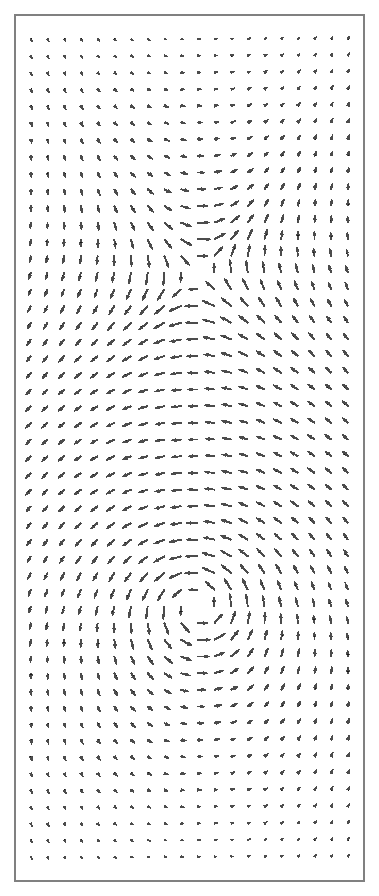
\includegraphics[width=0.5\textwidth]{figs/vortex.pdf}
	\begingroup
\setbox0=\hbox{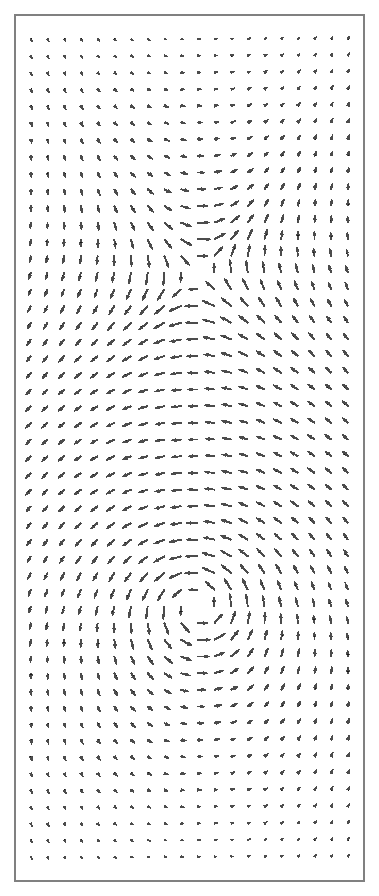
\includegraphics{figs/vortex.pdf}}%
\parbox{\wd0}{\box0}\endgroup
\end{titlepage}

\dominitoc 
\tableofcontents


\chapter{March}
\begin{tocbox}
	\minitoc
\end{tocbox}

\section{Metropolis-Hastings Monte Carlo}
We want to generate a set of samples from a distribution $ P(x) $. 
The goal is to use a Markov process that asymptotically reaches a distribution 
that coincides with $ P(x) $. 

We start with the detailed balanced condition: consider 
a system in thermal equilibrium, and two states $ x $ and $ x' $ of that system. 
The probability of being in state $ x $ and going from $ x $ to $ x' $ is the same as
the probability of being at $ x' $ and going back to state $ x $: 
\begin{equation}\label{eq:detailed-balance}
	P(x \rightarrow x') P(x) = P(x' \rightarrow x) P(x').
\end{equation}
Here $ P(x \rightarrow x') $ is occasionally written as $ P(x' \mid x) $, 
as in a Markov process we can consider the probability of going to $ x' $ 
\textit{given} a previous state $ x $. This is fact would require us to 
factor $ P(x' \mid x) $ into $ P(x' \mid x) = g(x' \mid x)A(x', x)$, 
where $ g(x' \mid x) $ captures the \textit{conditional probability of considering 
$ x' $ as the next state} that might arise if this process is such that the
probability distribution \textit{changes} depending on the previous state, and $
A(x', x) $ is the probability of actually making that transition. 
In statistical mechanics the equilibrium probability distribution does not
change depending on which of the states of the ensemble you're in, so the above is
not really a point of concern and we can unambiguously write $ P(x \rightarrow
x') $. 

The idea is to write \cref{eq:detailed-balance} as 
\begin{equation}\label{eq:ratio}
	\frac{P(x \rightarrow x')}{P(x' \rightarrow x)} = 
	\frac{P(x')}{P(x)}
\end{equation}
and to choose $ P(x \rightarrow x') $ and $ P(x' \rightarrow x) $ such that 
this condition is always fulfilled. An intuitive choice is the so-called 
\textit{Metropolis} choice, which is the most important bit to understand:
\begin{thinbluebox}
	\begin{equation*}
		P(x \rightarrow x')
		= \min \left( 1,
		\frac{P(x')}{P(x)}
		\right)
	\end{equation*}
Make the move from $ x $ to $ x' $ no matter what if $ P(x') > P(x) $ (i.e., 
if $ x' $ is a more likely state); make the move with probability $ P(x')/P(x) $
if it is a less likely state.
\end{thinbluebox}
Where in the algorithm we generate a random number between $ 0 $ and $ 1 $ 
and make the move if that number is less than $ P(x  \rightarrow x') $ (hence 
with certainty if $ P(x') > P(x) $ and with chance to $ P(x')/P(x) $
otherwise). Here implicitly the same choice is also made for $ P(x' \rightarrow x) $, 
where we just switch $ x \longleftrightarrow x' $ in the above definition (note 
that we only have to compute $ P(x \rightarrow x') $, though, since we are only 
considering the move from $ x $ to $ x' $).  This fulfilled \cref{eq:ratio} in
the following sense: 
\begin{itemize}
\item If $ P(x') > P(x) $, we set $ P(x \rightarrow x') = 1 $ and $ P(x'
	\rightarrow x)  = P(x)/ P(x')$. Then the ratio of $ P(x \rightarrow x') $ and $
	P(x' \rightarrow x) $ is the right hand side of \cref{eq:ratio}: 
	\begin{equation*}
		\frac{P(x \rightarrow x')}{P( x' \rightarrow x)} 
		= \frac{1}{P(x)/P(x')} 
		= \frac{P(x')}{P(x)}
	\end{equation*}
\item If $ P(x') < P(x) $, we set $ P(x \rightarrow x') = P(x')/{P(x)} $ and 
	$ P(x' \rightarrow x)  = 1$  and again the ratio \cref{eq:ratio} is satisfied.
\end{itemize}

The power in its application to statistical mechanics lies in the fact that we 
only need to compute the relative change in energy $ P(x')/P(x) $! E.g., 
in the Ising model with coordination number $ z $, if we are in an all-up (or
down) ferromagnetic state and flip spin $ k $:
\begin{align*}
	\frac{P(x')}{P(x)} = \frac{\exp\left(\beta J \sum S_i S_j \right)}{\exp\left(\beta J\sum S_iS_j\right)}
	= \frac{
		\cancel{\exp(\beta J\sum_{i,j\neq k}S_i S_j)}\cdot \exp \left( \beta J\sum_j S_j S_k \right)
	}{
		\cancel{\exp(\beta J\sum_{i,j\neq k}S_i S_j)}\cdot \exp \left(\beta J\sum_j S_j S_k \right)
		}\\
	= \frac{
		\exp \left(\beta J\sum_j (+1) (-1) \right)
	}{
		\exp \left( \beta J\sum_j (+1) (+1) \right)
	}
	= \frac{
		\exp \left( -z \beta J\right)
	}{
		\exp \left( z\beta J\right)
	}
	= \exp(-2zJ\beta).
\end{align*}

\section{Symmetries and Degeneracy}\label{sec:symmetries-degeneracy}
We use here the example of rotational symmetry, although the argument is general 
unless otherwise specified. Our goal is essentially to derive the $ m $
(magnetic quantum number) degeneracy present in central potentials/rotationally
invariant systems such as the hydrogen atom. Consider the $ (2\ell + 1)
$-dimensional irrep of  $ L_z $, the angular momentum operator. We know this
generates the group of rotations about the $ z $ axis by $ \exp(-i\theta L_z) $.
Consider also a Hamiltonian with $ z $-rotational symmetry. Then
\begin{equation*}
	e^{-i \theta L_z} H e^{i\theta L_z}	= H 
	\Longrightarrow  
	\left[ e^{i\theta L_z}, H\right] = 0 
\end{equation*}

\begin{wrapfigure}{r}{0.4\textwidth}
	\begin{center}
		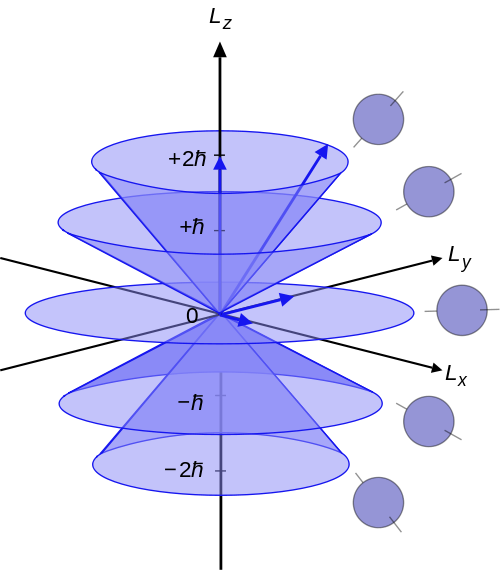
\includegraphics[width=0.4\textwidth]{figs/march/500px-Vector_model_of_orbital_angular_momentum.svg.png}
		\caption{}
		\label{fig:spin}
	\end{center}
	\vspace*{-4em}
\end{wrapfigure}

We can ascertain from this two facts: 
\begin{enumerate}[]
\item $ z $-rotated states are also eigenstates of $ H $ with the same 
	energy: $ \left[ e^{ i\theta L_z }, H \right] = 0 \Longrightarrow H e^{i\theta
	L_z}\ket{E_n} = e^{i\theta L_z} H\ket{E_n} $, so $H (e^{i\theta
	L_z}\ket{E_n}) = E_n (e^{i\theta L_z}\ket{E_n})$. In a sense this can 
	be thought of as a degeneracy, but this is not a particularly useful line of
	thinking: applying the rotation operator $ e^{i\theta L_z} $ does not alter
	the quantum numbers of $ E_n $ with respect to the quantization axis $ L_z$,
	so there are no other eigenstates of $ L_z $ with the same energy, and 
	this ``degeneracy'' is fictitious, so to speak. Besides, $ e^{i\theta L_z} $
	is not Hermitian and thus is not an observable.
\item Eigenstates of $ H $ are also eigenstates of $ L_z $: 
	$  \left[ e^{ i\theta L_z }, H \right] = 0 \Longrightarrow \left[ L_z, H \right]=0$.
	Note this does not mean that the $ L_z $-eigenvalues are the same as $ H $
	eigenvalues! That is, we've not yet derived the degeneracy; in fact, 
	if the eigenvalues were the same, we might've indeed derived a degenerate set 
	of states. What this does mean is that we can use both $ E_n $ and $ m $, $
	\ell $ to label the eigenstates.
\end{enumerate}
In reference to the latter fact, I will only use $ m $ henceforth, dropping the 
quantum number $ \ell $. This amounts to implicitly picking the irreducible 
representation of dimension $ 2\ell + 1 $ of the rotation group. 

So far we've only considered $ z $-rotational symmetry. This does not give us 
the degeneracy in $ m $. To do this, we need some more physical intuition: 
we know that the magnetic quantum number $ m $ roughly corresponds to the 
projection of the angular momentum along the $ z $ axis. Degeneracy in $ m $
corresponds to the Hamiltonian produce \textit{the same energies independent of
the direction of the angular momentum} (specifically, its projection along the 
$ z $ axis). To obtain this, the system needs to also be invariant with respect 
to rotations along the $ x $- and $ y $- axes, as such rotations will alter 
the projection along the $ z $-axis. See \cref{fig:spin}. This is the main insight: 

\begin{thinbluebox}
Symmetries lead to Hamiltonians that have solutions with the same energy related 
by a certain transformation. If that transformation changes a certain quantum 
number, it should be the case that those new states (labelled by the new quantum 
numbers) are also solutions with the same energies, and thus those transformations 
generate the degeneracy in that quantum number. 
\end{thinbluebox}
Then the generator $ L_x $ should correspond to the transformations that lead 
to the degeneracy. This is seen by considering the transformation law $ L_x =
\frac{1}{2}(L_+ + L_-) $ (again, if $ m $ is the projection along the $ z $ axis, 
we can see that rotations $ e^{i\theta L_x} $ increase, and, as a superposition, 
increase the projection of the angular momentum along the $ z $ axis, exactly as 
if we are rotating the angular momentum vector). Then, if the Hamiltonian is
symmetric with respect to $ x $-rotations, 
\begin{align*}
	L_x H\ket{E_n, m} &= HL_x\ket{E_n, m}\\
	\frac{1}{2} E_n(L_+ + L_-)\ket{E_n, m} 
		&= \frac{1}{2}H(L_+ + L_-)\ket{E_n, m} \\
	\frac{1}{2}E_n L_{\pm}\ket{E_n, m} 
		&= \frac{1}{2}H L_{\pm} \ket{E_n, m}
		&& (\ket{m\pm 1} \text{ are linearly indep.})\\
	E_n \ket{E_n, m\pm 1} 
		&= H \ket{E_n, m\pm 1}.
\end{align*}
Thus altering the value of $ m $ leads to another eigenstate with the same 
energy.

Some other remarks: its possible that the symmetry group we are considering 
is Abelian. In this case, it turns out that the irreducible representation 
is trivial (see here). This means that for Abelian symmetries, the state 
is only altered by an overall phase factor and there is no degeneracy:
if $ \left[ H, e^{it\theta} \right] =0$
\begin{equation*}
	E_ne^{it \phi}\ket{E_n} = He^{it \phi}\ket{E_n}
	\Longrightarrow \cancel{e^{it \phi}}E_n \ket{E_n}
		= \cancel{e^{it \phi}}H\ket{E_n}
	\Longrightarrow 
	E_n \ket{E_n} = H\ket{E_n}
\end{equation*}
where $ \phi $ is the one dimensional representation. The last equality, of
course is something we already knew. 

An example is that of a one-dimensional symmetric potential; the symmetry is 
$ \Z_2 $, which is Abelian. Such a system has no degeneracy. 

\begin{thinnamedbox}[LRL vector and $ \ell $ degeneracy]
Inverse-square potentials are known to have an additional conserved quantity, 
the Laplace-Runge-Lenz vector. This turns out to correspond to a 4-dimensional 
spherical symmetry, which in turn leads to a degeneracy in the $ \ell $ 
(azimuthal) quantum numbers, such as those present in the Hydrogen atom. 
\end{thinnamedbox}

\subsection*{See also}
\begin{itemize}
\item The examples section of
\href{https://www.uio.no/studier/emner/matnat/fys/FYS3110/h20/pensumliste/symmetry_degeneracy.pdf}{this
document.} 
\end{itemize}

\section{Connections, Generally}
There is a connection between connections (haha); that is, when we hear people 
refer to the potentials $ A_\mu $ as ``connections'' in gauge theory (quantum 
field theory), this actually does correspond to the Riemannian connection 
$ \del_X Y $ we see in differential geometry, and similarly for notions 
such as curvature, covariant derivatives, etc. 

There is one quick terminological clarification to make. What we refer to as 
a connection in gauge theory (e.g., $ A_\mu $) really corresponds to the 
Christoffel symbols $ \Gamma_{ij}^k $; the (gauge) covariant derivative 
is, under this terminology, really $ \del_X Y $. The reason the two are 
referred to interchangeably is that the $ \Gamma_{ij}^k $ can be thought 
of as implicitly determined upon specifying $ \del_{X}Y $, and vice-versa. 
It's not unlike how people will refer to the representation space as a 
``representation.'' Which infuriates me to this day. 

One discrepancy that might be concerning at first is the fact that, in 
gauge theory (let's generalize to non-Abelian here), the connection appears 
to have one index: e.g., in Peskin and Schroeder \S15.2 we see $ A_\mu^i $,
where $ i $ indexes the generator of the gauge symmetry group.
From \href{https://physics.stackexchange.com/questions/432640/is-%E2%88%82-mu-i-e-a-mu-a-covariant-derivative-in-the-differential-geometry-sen}{Stack Exchange}:

\begin{quotebox}
	Mathematicians would refer to a gauge theory setting as a fiber
	bundle. $ A_\mu $ takes the role of a connection on the fibre bundle. Of course,
	out of the three indices the Cristoffel symbols $ \Gamma^{i}_{jk} $ have, two
	indices ``live" in the fiber. You can appreciate this more easily if you look at
	non-Abelian gauge
	theories, in which $ (A_\mu)_{ij}  = A^a_\mu T_{ij}^a$
\end{quotebox}
So here $ (A_\mu)_{ij} $ corresponds to $ \Gamma_{jk}^i $.

To understand the correspondence between curvatures, we need an expression 
of the curvature of Riemannian geometry $ R(X,Y)Z $ in terms of the connection 
$ \Gamma_{ij}^k $. The bottom equation of page 92 of Do Carmo's
\textit{Riemannian Geometry} gives us what we need: 
\begin{equation}\label{eq:riemann-curvature}
	R(X_i, X_j)X_k = \del_{X_j}(\Gamma^{\ell}_{ik}X_\ell)
	- \del_{X_i}(\Gamma^{\ell}_{jk}X_\ell).
\end{equation}
($ X_i $ are basis vectors, so it's not difficult to convert to index notation
from this.)

\begin{itemize}
\item \textbf{Berry's phase:} The connection is the \textit{Berry connection}
	$ A^n(\vb{R}) = i \bra{n(\vb{R})} \partial_{\vb{R}}\ket{n(\vb{R})}$ 
	(\mycomm{what is the fiber bundle?}), from which we obtain the \textit{Berry
	curvature} $ \omega_{\mu\nu} (\vb{R}) = \partial_{R_\mu}A^n_\nu(\vb{R}) -
	\partial_{R_\nu} A^n_\mu (\vb{R})$. Cf. \cref{eq:riemann-curvature}; 
	the missing index relative to $ R(X_i, X_j)X_k $ comes from the fact 
	that we've written $ \vb{R} $ in the vector form as opposed to index 
	form. 
\end{itemize}


\subsection*{See also}
\begin{itemize}
\item Girvin and Yang's \textit{Modern Condensed Matter Physics}, \S 13.1 
	has an excellent explanation of Berry's phase. 
\item \href{https://arxiv.org/abs/hep-th/0611201}{These notes}.
\end{itemize}

% \section{PT Non-Hermitian Hamiltonians, Exceptional Points}
% I stumbled across this one in a funny way: Right after a talk Stephen Carr did on 
% the Moir\'e effect in condensed matter, once the room had well-vacated he
% mentioned to a faculty member that level-crossing is something we ``should
% really teach in our courses but don't.'' Under the impression that
% level-crossing is a fairly straightforward, 
% minor thing, I launched on a search for some paper or review elaborating on what 
% he mentioned. I did not succeed; as a matter of fact, at the time of writing 
% I am still looking for one such treatment. Instead I found a Stack Exchange post 
% on avoided crossings which had an answer mentioning ``exceptional points;'' 
% following one of the references in the Wikipedia page led me to a review 
% titled \textit{Exceptional Topology of Non-Hermitian Systems}, which made 
% use of (what I think is) a formalism for dissipative quantum systems,
% non-Hermitian effective Hamiltonians. This, in turn, led me to the subject at
% hand. Phew!

\section{Legendre Transforms}
This is one I've been meaning to sit down and understand more carefully for one
or two years, actually. It's a remarkably simple concept that somehow gets 
mangled by thoughtless pedagogy in almost every single treatment. 
The big idea is: we'd like to turn a function $ f(x) $ into a function of $
p = \dv*{f}{x} $. Put in other words, we can think of it as ``a map from the graph of 
the function ot the tangents of the graph'' (Wikipedia). 

\begin{wrapfigure}{r}{0.4\textwidth}
	\begin{center}
		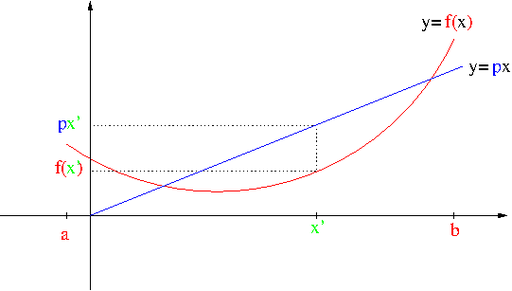
\includegraphics[width=0.4\textwidth]{figs/march/512px-Legendre_transformation.png}
		\caption{}
		\label{fig:legendre}
	\end{center}
	\vspace*{-4em}
\end{wrapfigure}
Say we have a convex function $ f(x) $ (in the case the function isn't convex
everywhere, we can restrict ourselves to an interval where it is convex), and a
line $ y=px + b $ which we'd like to make the tangent line of $ f(x) $ at $
x=x_0 $ by tweaking $ p $ and $ b $. For this to be the case,
\begin{align*}
	y = px + b = \dv{f}{x}\evalat_{x_0} x + b 
	\Longrightarrow p = \dv{f}{x}\evalat_{x_0}\\
	\qquad
	\text{and}\qquad 
	y(x=x_0)=p x_0 + b  = f(x_0)
\end{align*} 
(Note this is \textit{not} related to the Taylor series expansion, we're just 
looking for the tangent line at the point $ f(x_0) $). Since $ f(x) $ is convex
$ \dv*{f}{x} = p $ can be inverted, and we can solve for $ x_0 = (f')^{-1} (p)$. 
Now it remains to solve for $ b $ by using the last equality above: 
\begin{equation*}
	b = f(x_0) - px_0
\end{equation*}
Since we know $ x_0 = (f')^{-1}(p) $ and we're ultimately looking to convert 
$ f $ into a function of $ p $:
\begin{equation*}
	b = f((f')^{-1}(p)) - p \cdot (f')^{-1} (p)
	\equiv f^\ast(p)
\end{equation*}
were we've defined the Legendre transform in the last equality. As it turns out,
the value of $ x_0 $ is such that the distance between $ f(x_0) $ and 
$ px_0 $ is maximized: we could have found $ x_0 $ as a function of $ p $ 
by maximizing $ b=b(x) $:
\begin{align*}
	b(x) = f(x) - px 
	&\Longrightarrow \pdv{b}{x}\evalat_{x_0} = f'(x_0) - p = 0 \\
	&\Longrightarrow x_0 = (f')^{-1}(p),
\end{align*}
which is what commonly drawn figures such as \cref{fig:legendre}
are trying to tell you.

\begin{thinbluebox}
The Legendre transform is defined by 
\begin{equation*}
	f^\ast(p) = f(x_0) - px_0, 
	\qquad x_0 = (f')^{-1}(p),
\end{equation*}
It states that for a convex function $ f $ we can determine the function's 
tangent lines' $ y $-intercepts for given values $ p $ of their slopes.
$ f^\ast(p) $ is precisely the $ y $-intercept of the function for a slope $ p $.
\end{thinbluebox}

\href{https://www.desmos.com/calculator/fmvcupzb4t}{Here's} an interactive 
Desmos graph that demonstrates this. In this sense it is a very simple 
procedure---one a high school calculus student could discover by accident if, 
say, they are trying to make an animation of a tangent line coasting along 
the plot of a function. 

This revisit was informed by an issue Elijah brought up. It was something like: 
one encounters a ``path integral'' with ``Lagrangian'' $ \pi \phi - H[\pi, \phi] $
integrated over both the field \textit{and} the canonical momentum $ \pi $; 
this it \textit{not} the usual path integral, as there is a mysterious 
integration over $ \pi $. We were curious as to why. The answer is that the 
the Legendre transform exchanges 
\begin{equation*}
	H(p, q) \longleftrightarrow L(\dot{q}, q), 
	\qquad 
	\text{i.e.,}\qquad p \longleftrightarrow \dot{q},
\end{equation*}
where $ p\equiv\pdv*{L}{\dot{q}} $ \textit{is evaluated at a point specified by
$ q $, $ t $}, so properly it should be written $ \pdv*{L}{q}\vert_{\dot{q}_0,
q, t} $. This is why the path integral resulting from the proper Legendre
transform only includes integration over the field $ \phi $, $ \pi $ is
implicitly given by $ \phi $. 

\chapter{April}
\begin{tocbox}
\minitoc
\end{tocbox}

\section{Miscellaneous Bash Things}
\subsection{How to run a command without admin}
E.g., using the \href{https://www.tug.org/mactex/morepackages.html}{BasicTeX}
distribution of \LaTeX, I used to have to write \mintinline{shell}{sudo tlmgr install} 
every time I wanted to install a package. You can fix this by (1) giving yourself 
(or any user) ``no password'' privilege to run that specific command, then (2)
\textit{alias} the command \mintinline{shell}{sudo tlmgr} to just
\mintinline{shell}{tlmgr}.

Specifically, step (1) is to add the following line to the \mintinline{shell}{/etc/sudoers}
file, which controls what users have which \mintinline{shell}{sudo} privilege to 
do what: 
\begin{minted}{shell}
<username> ALL = (root) NOPASSWD: <command>
\end{minted}
Note that \mintinline{shell}{<command>} requires the \textit{full} path to the executable.
Also note that you should place this after the root specifications. See \href{https://askubuntu.com/questions/100051/why-is-sudoers-nopasswd-option-not-working}{this}.


Step (2) is to make the shell alias your command on startup by adding the following 
line to \mintinline{shell}{~/.bashrc} (or \mintinline{shell}{~/.zshrc}): 
\begin{minted}{shell}
alias <command>='sudo <command>'
\end{minted}

From \href{https://superuser.com/questions/1495807/can-someone-explain-what-is-user-all-all-nopasswdall-does-in-sudoers-file}{Stack Exchange}, 
\mintinline{shell}{sudoers} formatting is:
\begin{quotebox}
	\begin{minted}{shell}
user_spec host_spec = (runas_spec) NOPASSWD:cmd_spec
	\end{minted}
	\begin{itemize}
	\item \mintinline{shell}{user_spec}: which users can use the rule 
	\item \mintinline{shell}{host_spec}: which hosts the rule applies 
		to. This is optional and defaults to all. 
	\item \mintinline{shell}{runas_spec}: which users the commands can be run 
		as. 
	\item \mintinline{shell}{NOPASSWD} or \mintinline{shell}{PASSWD}: 
		whether a password is required. Optional and defaults to \mintinline{shell}{PASSWD}
		unless the default has been changed in the sudeors configuration. 
	\item \mintinline{shell}{cmd_spec}: identifies which commands the rule can 
		be run for. 
	\end{itemize}
\end{quotebox}

\subsection{Running a terminal script in the background}
Say you have an application that is started on the terminal and runs in a GUI 
or something, and you want to close the terminal while still using the
application; you can start it, then 
\begin{enumerate}
	\item Use Ctrl-Z to suspend it
	\item Use \mintinline{shell}{bg} to make it a background job
	\item Run \mintinline{shell}{disown} to remove the job from the current
	shell
	\item Feel free to then close the terminal.
\end{enumerate}

If you want to start the script already in the background in such a way that 
logout doesn't terminate the script, you can add a \mintinline{shell}{&} to the 
end, which automatically backgrounds (i.e., runs \mintinline{shell}{bg}) it, and
run it in ``no hangup'' mode \mintinline{shell}{nohup} such that it stays
running and outputs everything to a file called \mintinline{shell}{nohup.out};
e.g., 
\begin{minted}{shell}
nohup qitview &
\end{minted}

\section{Solving a ODE as a Matrix Problem}
I find that the matrix method in, say, computational single-particle quantum 
mechanics, is rarely derived in a nice explicit way. Here's a quick calculation 
that makes it more unambiguous. Do a backward and forward Taylor expansion:
\begin{align*}
	\psi(x_i + \Delta x) \approx \psi(x_i) + \frac{d\psi}{dx}\evalat_{x_i}\Delta x 
		+ \frac{1}{2} \frac{d^2\psi}{dx^2}\evalat_{x_i}(\Delta x)^2\\
	\psi(x_i - \Delta x) \approx \psi(x_i) - \frac{d\psi}{dx}\evalat_{x_i}\Delta x 
		+ \frac{1}{2} \frac{d^2\psi}{dx^2}\evalat_{x_i}(\Delta x)^2
\end{align*}
Call $ \psi(x_i\pm \Delta x) \equiv \psi_{i\pm 1}$ and add these two equations:
\begin{equation*}
	\psi_{i+1} + \psi_{i-1} \approx 2\psi_i 
		+ \frac{d^2\psi}{dx^2}\evalat_{x_i}(\Delta x)^2
	\Longrightarrow \frac{d^2\psi}{dx^2}\evalat_{x_i} \approx 
		\frac{\psi_{i+1} + \psi_{i-2} - 2\psi_i}{(\Delta x)^2}
\end{equation*}
Now we can obtain an approximate matrix representation of the second derivative
\begin{align*}
	&\frac{1}{(\Delta x)} \sum_i D_{ij}\psi_{i} = \frac{1}{(\Delta x)^2}
		\qty( \psi_{i+1} + \psi_{i-1} - 2\psi_i )
	= \frac{1}{(\Delta x)^2}
		\sum_i \qty( \delta_{j(i+1)} + \delta_{j(i-1)} - 2 \delta_{ij} ) \psi_i\\
	&\qquad \qquad \Longrightarrow 
	\mathbox{D_{ij} = \delta_{j(i+1)} + \delta_{j(i-1)} - 2 \delta_{ij} }
\end{align*}
which is a tridiagonal or band matrix. 

\chapter{May} 
\begin{tocbox}
\minitoc
\end{tocbox}

\section{Carroll 3.6: Curvature Approach to Satellite Orbit}
The metric outside the earth can be approximated by 
\begin{equation*}
	\dd{s}^2 = -(1+2\Phi)\dd{t}^2 + (1-2\Phi)\dd{r}^2 
		+ r^2 (\dd{\theta}^2 + \sin^2\dd{\phi}^2), \qquad 
		\Phi = -\frac{GM}{r}
\end{equation*}
First, we can compute the flow of time at radii $ R_1 $ and $ R_2 $. This is 
done by picking a rest frame at a point with radius $ R_{1,2} $ such that 
$ \dd{r} = \dd{\phi} = \dd{\theta} = 0 $. So the expression for the metric 
reduces to 
\begin{equation*}
	\dd{s}^2 = -(1+2\Phi_{1,2})\dd{t}^2.
\end{equation*}
We have just two degrees of freedom so that we can solve it as a differential 
equation. In fact, since we're working in the rest frame, the arclength $ s $ 
is exactly the proper time $ \tau_{1,2} $. Taking the square root of both 
sides (properly, giving both sides some vector as described in Carroll \S 2.6)
\begin{equation*}
	\dd{\tau_{1,2}} = \sqrt{-(1+2\Phi_{1,2})}\dd{t}
\end{equation*}
We then integrate both sides to obtain 
\begin{equation*}
	\tau_{1,2} = \sqrt{-1-2\Phi_{1,2}} t
\end{equation*}
So that we can find 
\begin{equation*}
	\tau_{1} = \qty[ \frac{R_2(2GM - R_1)}{R_1(2GM-R_2)} ]^{1/2}\tau_2
\end{equation*}
If $ R_2>R_1 $, the coefficient is greater than one and we find that time passes 
faster farther away from earth.

Now suppose that there's a particle orbiting the earth at a fixed radius and 
$ \theta = \pi/2 $. In this case $ \dd{t}\neq 0 $ and $ \dd{\phi} = 0 $; there 
are two nonvanishing differentials and we can't approach the problem like we did 
above. We will need to use the geodesic equation
\begin{equation*}
	\dv[2]{r}{\lambda} + \Gamma_{\rho\sigma}^{r} \dv{x^\rho}{\lambda}
		\dv{x^\sigma}{\lambda} = 0
\end{equation*}
We can assume that in this orbit $ \dd{\phi}{t} $ is some constant $ \omega $. 
Then the only relevant geodesic equation is for $ \dv*[2]{r}{\lambda} $.
Since $ r $ is fixed, $ \dv*{r}{\lambda} = \dv*[2]{r}{\lambda} =0 $, and
similarly for $ \theta $.  The only relevant Christoffel symbols are then $
\Gamma_{\phi\phi}^r $ and $ \Gamma_{tt}^r $; the remaining terms in the geodesic
equation above vanish. The geodesic equation becomes 
\begin{equation*}
	\Gamma_{\phi\phi}^r \qty( \dv{\phi}{\lambda} )^2 
		+ \Gamma_{tt}^r \qty( \dv{t}{\lambda} )^2 = 0
\end{equation*}
There is no time dependence in any of the elements of the metric and thus 
$ t $ is equal to $ \lambda $ times some constant of proportionality. Applying 
the chain rule to all terms above and cancelling the factors of $ (\dv*{\lambda}{t})^2 $
finds 
\begin{equation*}
	\Gamma_{\phi\phi}^r\dot{\phi}^2 + \Gamma_{tt}^r = 0
\end{equation*}
Substituting $ \dv*{\phi}{t} = \omega $ and solving for it yields 
\begin{equation*}
	\omega = \sqrt{\frac{\Gamma_{tt}^r}{\Gamma_{\phi\phi}^r}}
\end{equation*}

Lastly, we can determine the proper time elapsed per complete orbit for someone 
on the surface of the earth as compared to the orbiting particle itself. 
We will have to use the expression for the proper time: 
\begin{equation*}
	\tau = \int \qty( -g_{\mu\nu} \dv{x^\mu}{\lambda} \dv{x^\nu}{\lambda} )^{1/2}
		\dd{\lambda}.
\end{equation*}
In our case an observer on earth will find 
\begin{equation*}
	\tau_{\text{E}} = \int\qty[ (1+2\Phi) - r^2 \omega^2 ]^{1/2}\dd{t}
		= \sqrt{(1+2\Phi) - r^2\omega^2} \cdot t
\end{equation*}
(we've again used the fact that we can reparameterize from $ \lambda $ to $ t $).

\section{Comments on Killing Vectors}
The Killing vectors of Minkowski spacetime are precisely the Lie algebra of 
the Poincar\'e group: 
\begin{itemize}
\item Time and space translations $ \partial_\mu $. 
\item Rotation generators $ - x_i \partial_j + x_j \partial_i $.
\item Boost generators $ x_i\partial_0 + x_0 \partial_i $.
\end{itemize}
The boost generators (and, I think the rotation generators as well) can be 
seen to have the above form by considering a very small boost by a rapidity 
$ \phi $. For this purpose we can jettison the two other spatial coordinates 
and just focus on one spatial direction. Then the boost is
\begin{equation*}
	\begin{bmatrix}
		t'\\x'
	\end{bmatrix}
	= 
	\begin{bmatrix}
		\cosh\phi & -\sin\phi \\ \sinh\phi & \cosh\phi
	\end{bmatrix}
	\begin{bmatrix}
	t\\x
	\end{bmatrix}
	\approx 
	\begin{bmatrix}
	1 & -\phi \\ \phi & 1
	\end{bmatrix}
	\begin{bmatrix}
	t\\x
	\end{bmatrix}
	 = \begin{bmatrix}
	 t\\x
	 \end{bmatrix}
	  + \phi \begin{bmatrix}
	  x \\ t 
	  \end{bmatrix}
\end{equation*}
writing the second vector (without the $ \phi $ prefactor) in the standard
differential geometric notation recovers $ x_i \partial_0 + x_0\partial x_i $.
The procedure is analogous for the other elements of the Lie algebra, e.g., 
$ \partial_\mu $ comes from 
\begin{equation*}
	\begin{bmatrix}
	t' \\ x'
	\end{bmatrix}
	\approx 
	\begin{bmatrix}
	t\\x 
	\end{bmatrix}
	+ \delta x  
	\begin{bmatrix}
	0 \\ 1
	\end{bmatrix}.
\end{equation*}
\mycomm{The precise connection to the exponential map in Lie theory is not crystal clear 
to me (especially when in Hilbert space); I assume the matrices multiplying our 
vectors above (e.g., the rapidity matrix) is the matrix exponential which 
for a small parameter turns approximately into a simple linear transformation as above,
but according to that picture the generators should be matrices (operators), not
vectors as we see here. Will investigate further when I have time.}

\subsection{Static and Stationary Spacetimes}
A metric is called stationary if it has a timelike Killing vector, which 
essentially means that you can find observers such that the spacetime is 
unchanging. A static metric (or static spacetime) is that of a spacetime that is 
additionally irrotational. It turns out that an equivalent definition of a static 
metric is a stationary metric that is symmetric with respect to $ \partial_t 
\rightarrow -\partial_t $, or, alternatively, a metric such that $ \partial_t $ 
is everywhere orthogonal to a spacelike hypersurface. We can show these two 
definitions are equivalent. 

Some preliminaries: a vector $ v_\mu $ orthogonal to a hypersurface of constant 
$ f $ can be written $ v_\mu = h \del_\mu f = h \partial_\mu f $ for a function 
$ h $ (we can write it in terms of a regular partial derivative because a function 
is a rank-$ (0, 0) $ tensor). The Frobenius theorem then tells us we can write 
\begin{equation}
	v_{[\sigma}\del_\mu v_{\nu]} = 0
\end{equation}
The proof is simple; just write $ v_\mu = h\del_\mu f $ and use the fact that the 
covariant derivative commutes when applied to functions. Lastly, note the
Killing equation can be written as $ \mathcal{L}_\xi g_{\mu\nu} $ for a Killing 
vector $ \xi $ (this just says that the metric tensor doesn't change along a Killing 
vector, the defining property of Killing vectors). 

One last fact that we need: if $ \xi $ is timelike, we can write it $ \partial_t $
for some choice of coordinates. Expanding the Lie derivative above and substituting 
$ \xi=\partial_t $: 
\begin{equation*}
	\mathcal{L}_\xi g = \partial_\gamma g_{\alpha \beta} \cdot \xi^\gamma
		- g_{\mu\beta}\partial_\mu \xi^\alpha 
		+ g_{\alpha\mu} \partial_\beta \xi^\mu
	= 0 \quad\Longrightarrow \quad
	\partial_\gamma g_{\alpha \beta} \xi^\gamma
	= 0 \quad \Longrightarrow \quad 
	\partial_t g_{\alpha\beta} = 0
\end{equation*}
This means that if $ \xi $ is timelike, the metric should be independent of 
time. 

Now, to show that if the metric is symmetric with respect to $ \partial_t
\rightarrow -\partial_t $, $ \partial_t $ is everywhere orthogonal to spacelike 
hypersurfaces. Note that if the metric has this symmetry, there can be no 
terms in $ \dd{s} $ linear to $ \dd{t} $, since this transformation has 
$ \dd{t} \rightarrow -\dd{t} $. This means that $ g_{0i} = 0 $ for all spatial 
components $ i $. Then, it is a covariant fact of the matter that
\begin{equation*}
	g_{\mu\nu}\xi^\mu = g_{0\nu} = \delta_\nu^0
\end{equation*}
where in the last equation we used $ g_{0i} $. This is true everywhere and 
thus we can write $ \xi $ as the covariant derivative of some function of constant 
$ t $. 

Now show hypersurface orthogonality implies reversal symmetry. We can write 
$ \xi_\mu = \xi^2 \del_\mu f = \xi^2 \partial_\mu f $\footnote{At least I'm
pretty sure you can; I justify it by noting it's still the case that $ \xi
=\partial_t $ by hypothesis, which means we can choose $ f $ such that $
\partial_\mu $ has unit length.}. Since $ \xi^2 = g_{\mu\nu}\xi^\mu \xi^\nu = g_{tt} $
and  $ \xi_\mu = g_{\mu\nu}\xi^\nu  = g_{0\nu}$ in these coordinates, this 
equation is equivalent to 
\begin{equation*}
	g_{0\mu} = \partial_\mu f \Longrightarrow g_{00} = g_{00} \partial_\mu f
	\Longrightarrow \partial_0 f = 1
\end{equation*}
Solving this equation, we find 
	$ f = t + g(\vb{x}) $
for some arbitrary function $ g(\vb{x}) $ of the spatial coordinates. Now if we 
transform coordinates $ t \rightarrow t' = t- g(\vb{x}) $ and plug into our equation 
above again 
\begin{equation*}
	g_{0i}' = g_{00}' \partial_i (t' - g(\vb{x}) + g(\vb{x}))
		= g_{00}'\partial_i t' = 0
\end{equation*}
which we showed above is equivalent to the metric being time-reversal symmetric. 
This transformation preserves the Killing vector, since 
\begin{equation*}
	\xi^{\mu'} = \frac{\partial x^{\mu'}}{\partial x^\mu} \xi^\mu
		= \frac{\partial x^{\mu'}}{\partial x^0} \xi^0 
		= \frac{\partial t'}{\partial t} \delta_{0}^{\mu'}
		= (1, 0, 0 ,0).
\end{equation*}
so we can repeat the argument above to show the metric remains independent of $ t' $

This transformation does change the metric, though (hence we wrote $ g
\rightarrow g' $), because $ \dd{t'} = \dd{t} - \dd{g} $. However, this does not
ultimately matter; we are free to choose whatever coordinates make demonstrating
a certain fact most convenient and the geometry should remain the same, as the
changes in coordinates are appropriately accounted for by the Jacobian, etc.

\section{Canonical Density Matrix with Truncated Spectrum}
This is something I ran into working with data from finite-temperature trials of
SU(2) spin chains. The upshot is that if we are trying to compute the canonical density 
matrix $ e^{-\beta H} $ such a chain, the computed density matrix is inaccurate
when we don't have access to the full spectrum (such as with sparse
diagonalizations), and the error depends on chain size and temperature.

Recall by the Lieb-Schultz-Mattis theorem the
energy gap will vanish as we increase the number of sites (it goes as 1/N). Also
recall that the Boltzmann weights go as $e^{-\beta E_i}$. 

What this means is that as we crank up the number of sites while keeping
$\beta$, the gap will start to close and we will tend to sample higher and
higher energy eigenstates (i.e., states further up the spectrum). The issue is
if we only include a few eigenstates (as we would need to in a sparse matrix
diagonalization) the canonical density matrix would require more and more higher
energy eigenstates that are missing in the numerics. 

Note that if we keep our value of $\beta$ at the same scale as the energy gap,
then the temperature range shrinks with the energy gap and we don't need to
worry about sampling states that are not included in our numerics (because the
exponential would scale with the gap and those states would remain in the
vanishing tail of the distribution). This is what Alex meant by "currently, my
temperature scale is the width of the whole spectrum rather than the gap..."

\chapter{September}
\begin{tocbox}
\minitoc
\end{tocbox}

\section{Spontaneous Parametric Down-Conversion}
\begin{wrapfigure}{r}{0.4\textwidth}
	\begin{center}
		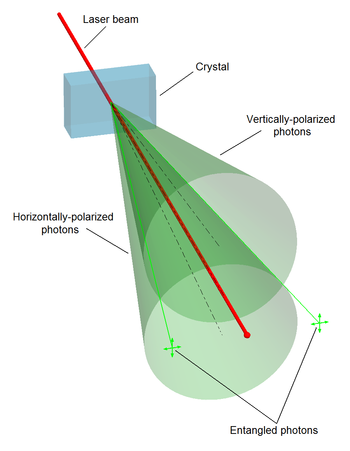
\includegraphics[width=0.4\textwidth]{figs/september/350px-SPDC_figure.png}
		\caption{}
		\label{fig:spdc}
	\end{center}
	\vspace*{-4em}
\end{wrapfigure}

I have been working in the instructional labs at Brown setting up a demonstration 
of Bell's inequality. We are using type II Spontaneous Parametric
Down-Conversion (SPDC), a nonlinear optical phenomenon which produces pairs of photons
entangled in the polarization basis. In our case we are using a barium borate
(BBO) crystal. 

The crystal produces two cones of photons bearing horizontal (ordinary) and 
vertical (extraordinary polarizations). One of these photons is referred to as 
the idler photon and the other the signal photon. The incoming photon is 
referred to as a pump photon. The effective Hamiltonian is 
\begin{equation*}
	H = i\hbar \kappa 
		\left(
			a_i a_s a_p^\dagger e^{i\Delta \vb{k}\cdot \vb{r} - i\Delta \omega \cdot t}
			+ a_i^\dagger a_s^\dagger a_p 
				e^{-i\Delta \vb{k}\cdot \vb{r} + i\Delta \omega \cdot t}
		\right)
\end{equation*}
where $ \Delta \omega = \omega_p - \omega_i - \omega_s $, $ a_i $ creates an
idler photon, so on. In the case of Type II SPDC, the nonlinear crystal produces
the two photons in two cones corresponding to horizontal and vertical
polarizations; the origin of these cones lies of course in conservation of
momentum. The cone the photon is in is therefore perfectly correlated with the
polarization, and if we know the cone, we know the polarization. 
The exception is the intersection of the two cones, where photons of either
polarization could be found. Since the photons are in this case
indistinguishable, the state 
of the system must be symmetrized and we have 
\begin{equation*}
	\ket{\psi} = \ket{H_i}\ket{V_s} + \ket{V_i}\ket{H_s}.
\end{equation*}

We can then test Bell's inequality by looking for \textit{coincident}
(simultaneously arriving) photons hitting our detectors, which should be entangled. 
{\color{myred} There's also an arbitrary phase in front of the second term above, 
which I've set to $ 1 $. Don't really understand why.}

\subsection*{Sources}
\begin{itemize}
	\item C. Cocteau, \href{https://arxiv.org/abs/1809.00127}{Spontaneous Parametric Down-Conversion}.
\end{itemize}

\section{Some Combinatorics Intuitions}
\parhead{Binomial coefficient} How might we construct the formula for $ n $
choose $ k $? We start with the number of permutations of the objects, then 
divide by the objects in the collection we don't care about. This is $ n!/(n-k)! $, 
so there are $ n $ ways to choose the first object, $ n-1 $ ways to choose the 
second, and so on until we've chosen $ k $, so we truncate at $ n-k $. But we also 
decide that the order doesn't matter, so we must divide by $ k! $ to eliminate 
the counts from the different permutations of those $ k! $ objects we picked.
\vspace*{2em}
\begin{equation*}
n \text{ choose } k = 
\begin{pmatrix}
n \\ k 
\end{pmatrix}	
= 
\frac{\eqnmarkbox[myblue]{node1}{n!}}{\eqnmarkbox[mygreen]{node2}{k!} \eqnmarkbox[myred]{node3}{(n-k)!}}
\end{equation*}
\annotate[yshift=1em]{}{node1}{permutation}
\annotate[yshift=-0.5em]{below,left}{node2}{accounts for order not mattering}
\annotate[yshift=-0.5em]{below,right}{node3}{eliminates objects we're not considering}
\medskip

\parhead{\dots with ordering} This suggests a simple way to get
the number of possible choices \textit{keeping track of order}: just get 
rid of the factor that eliminates the ``ordering equivalence''
\begin{equation*}
	\frac{n!}{(n-k)!}.
\end{equation*}

\parhead{\dots with replacement} Now say we choose $ r $ objects from a collection 
of $ n $ \textit{with replacement}. We keep the $ r! $ in the numerator to 
ignore ordering. We are sampling $ r $ times from that collection of objects, 
so to sample with repetition we have to add that object back into the collection 
for every time we sample. Since the collection \textit{already starts} with 
the object, we add $ r-1 $ (not $ r $), so the numerator takes on $ (n+r-1)! $. 
The numerator then goes to $ (n - k)! $ to $ ((n+ r - 1) - r)! $ so as to 
serve the same function as before, getting rid of the objects we're not 
sampling. 
\vspace*{2em}
\begin{equation*}
n \text{ choose } k = 
\begin{pmatrix}
n \\ k 
\end{pmatrix}	
= 
\frac{\eqnmarkbox[myblue]{node4}{(n+r-1)!}}{\eqnmarkbox[mygreen]{node5}{r!} \eqnmarkbox[myred]{node6}{(n-1)!}}
\end{equation*}
\annotate[yshift=1em]{}{node4}{permuatation replacing $ r-1 $ times}
\annotate[yshift=-0.5em]{below,left}{node5}{accounts for order not mattering}
\annotate[yshift=-0.5em]{below,right}{node6}{from $ (n+r-1-r) $}

\section{Noether's Theorem and Time-Dependent Symmetries}
\begin{wrapfigure}{r}{0.4\textwidth}
	\begin{center}
		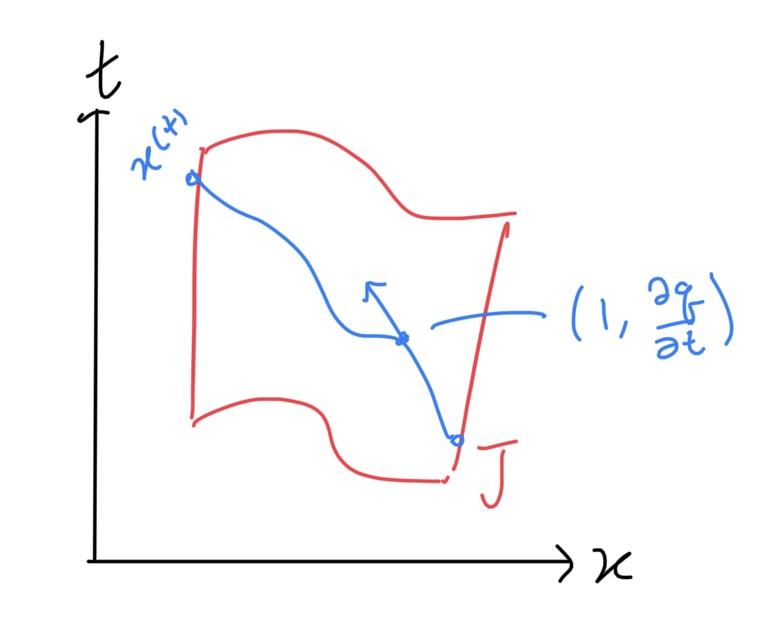
\includegraphics[width=0.4\textwidth]{figs/september/IMG_0030.jpg}
		\caption{}
		\label{fig:poisson}
	\end{center}
	\vspace*{-4em}
\end{wrapfigure}
The upshot is that the conserved quantity $ J $ has nonvanishing partial 
derivative but its Poisson bracket compensates such that the total derivative 
vanishes
\begin{equation*}
	\frac{\partial J}{\partial t} = 0,
	\quad\text{but}\quad
	\frac{d J}{d t} = -\left\{H, K\right\} + \frac{\partial J}{\partial t}= 0
\end{equation*}
Here is a differential geometric way of viewing the above equation: consider 
some space with coordinates $ (q,p,t) $, and some trajectory $ q(t) = x(t)  $, and some 
function $ J $ on this manifold. The differential/exterior derivative of $ J $ 
is 
\begin{align*}
	&\dd{J} = \frac{\partial J}{\partial x}\dd{x} + \frac{\partial J}{\partial p}\dd{p}
	+ \frac{\partial J}{\partial t}\dd{t}\\
		\Longrightarrow  &\frac{d J}{d t} = \frac{\partial J}{\partial q} \frac{\partial q}{\partial t}
			+ \frac{\partial J}{\partial p} \frac{\partial p}{\partial t}
			+ \frac{\partial J}{\partial t}
\end{align*}
Using Hamilton's equations $ \dot{q} = \partial H / \partial p $ and 
$ \dot{p} = - \partial H/ \partial q $, we find 
\begin{equation}\label{eq:eom}
	\frac{d J}{d t} = \frac{\partial J}{\partial q} \frac{\partial H}{\partial p}
		- \frac{\partial J}{\partial p} \frac{\partial H}{\partial q}
		+ \frac{\partial J}{\partial t}
		= -\left\{H,K\right\} + \frac{\partial J}{\partial t}
\end{equation}
This is represented in cartoon form by \cref{fig:poisson}.

\parhead{Galilean Boost} The Galilean boost is of the form $ x \rightarrow x+vt $, 
which is a symmetry of Newtonian mechanics. The conserved quantity is 
\begin{equation*}
	mx_\text{COM} - pt = \text{const.}
	\Longrightarrow  
	mx_\text{COM} = \text{const.} + pt
\end{equation*}
I.e., the center of mass moves according to the total momentum. The special 
relativistic analogue is that the conserved quantity of the Lorenz boost 
is the center of mass-energy.
We can work out \cref{eq:eom} for $ J = mx_\text{com} - pt  $, with $ H=p^2/2m $:
\begin{align*}
	\frac{d J}{dt}
		&= \frac{\partial }{\partial x}(mx_{\text{COM}} -pt)
			\cdot \frac{\partial }{\partial p} \left(\frac{p^2}{2m}\right) 
			- \frac{\partial }{\partial p} (mx_\text{COM} - pt) \cdot 
			\cancel{\frac{\partial }{\partial x}\left(\frac{p^2}{2m}\right)}
			+ \frac{\partial }{\partial p}(-pt)\\
		&= m\cdot \frac{p}{m} - p = p - p = 0.
\end{align*}

\section{Cosmological Constant}
Consider some nonvanishing vacuum energy-momentum tensor $ T^{\mu\nu} $. 
We postulate the vacuum is frame-independent (Lorentz-invariant), and also 
know that the only rank-two tensor that is Lorentz invariant is the metric. {\color{myred}(This is
``lore'' but I'm not sure what the proof is.)} (The invariance of the metric is 
what \textit{defines} Lorentz transformations). $ T^{\mu\nu} $ is then of 
the form 
\begin{equation*}
	T^{\mu\nu} = E g^{\mu\nu}
\end{equation*}
Then write a new general energy-momentum tensor capturing the vacuum energy: 
\begin{equation*}
	T^{\mu\nu} \rightarrow T^{\mu\nu} + E g^{\mu\nu}
\end{equation*}
and the Einstein equation becomes 
\begin{equation*}
	G^{\mu\nu} = \kappa (T^{\mu\nu} + E g^\mu\nu)
	\Longrightarrow G^{\mu\nu} - \kappa E g^{\mu\nu} = \kappa T^{\mu\nu}
\end{equation*}
setting $ -\kappa E=\Lambda $ recovers the usual form of the Einstein equation 
with a cosmological constant. The whole ``cosmological constant'' problem 
is that the vacuum energy of most quantum field theories yields a much 
larger cosmological constant than is actually observed.

\section{Newton-Cartan Gravity}
% TODO

\chapter{October}
\begin{tocbox}
	\minitoc
\end{tocbox}

\section{The Higgs Mechanism}
\parhead{Gauging a symmetry} Consider the linear sigma model 
\begin{equation*}
	\mathcal{L} = (\partial_\mu \phi^\ast)(\partial_\mu \phi)
			+ m^2 \phi\phi^\ast - \frac{\lambda}{4} \phi^2 \phi^{\ast 2}
\end{equation*}
which has a $ U(1) $ symmetry. We now ``gauge'' this symmetry by promoting 
to a local transformation: $ \phi \rightarrow e^{i\alpha(x)} \phi$. To do this 
we need to 
\begin{itemize}[noitemsep,topsep=0pt]
\item make the kinetic terms covariant wrt the gauge field and change 
	$ \partial_\mu \rightarrow D_\mu $, 
\item and introduce the corresponding dynamical 
	term for the gauge field:
\end{itemize}
\begin{equation*}
	\mathcal{L} = -\frac{1}{4}F_{\mu\nu}
		+ D_\mu \phi^\ast D_\mu\phi + m^2 |\phi|^2 - \frac{\lambda}{4}|\phi|^4
\end{equation*}
For a non-Abelian theory we'd have 
\begin{equation*}
	\mathcal{L} = -\frac{1}{4}F^{(a)\mu\nu}F_{\mu\nu}^{(a)}
		+ (\partial_\mu \phi^\ast - ieA^{(a)}_\mu(x) T^{(a)})
		  (\partial_\mu \phi + ieA^{(a)}_\mu(x) T^{(a)}) + \cdots 
\end{equation*}
In differential geometric language, recall that the fields $ \phi $ are 
sections of the (in this case, vector) bundle, $ A_\mu(x) $ are the connections 
corresponding to the principal $ G $ bundle where $ G $ is the Lie group of this 
theory.

\parhead{Higgs mechanism} Recall that spontaneous symmetry breaking puts us in
some classical minimum configuration which we can write as 
\begin{equation*}
	\phi(x) = \left(\frac{v+\sigma(x)}{\sqrt{2}}\right) e^{i\pi(x)/F_\pi}
\end{equation*}
where $ \pi(x) $ is the massless Goldstone boson (colloquially referred to as a pion) which will eventually be 
``eaten'' by the gauge boson to gain mass,
Now focus on the kinetic term only
\begin{equation*}
	-\frac{1}{4} F_{\mu\nu}^2 +  \left(\frac{v+\sigma}{\sqrt{2}}\right)^2 
		\left[-i \frac{\partial_\mu \pi}{F_\pi} + \frac{\partial_\mu \sigma}{v+\sigma}
			+ ieA_\mu\right]^2
\end{equation*}
This quadratic factor with three terms in the brackets will mix the dynamics 
of the three fields $ A_\mu $, $ \pi $, and $ \sigma $, but we single out the 
behavior of $ A_\mu $ and $ \pi $ by considering the sector where $ \sigma $
becomes decoupled from the other two fields. This is the so-called \textbf{decoupling 
limit}, which is achieved by giving $ \sigma $ an infinite mass $ m \rightarrow \infty $. 
Then $ \sigma $ is not at all dynamical and we can set it to zero. 
The potential term, had we included it, would have been 
\begin{equation*}
	-m^2 \sigma^2 - \frac{1}{2}\sqrt{\lambda} \sigma^3
		- \frac{1}{16}\lambda\sigma^4
\end{equation*}
which shows that $ m \rightarrow \infty $ is the right limit. The kinetic 
term then becomes 
\begin{equation*}
	\frac{v^2}{2}\left[i \frac{\partial_\mu \pi}{F_\pi} + ieA_\mu\right]^2
	= -
	\frac{v^2e^2}{2}\left[ \frac{\partial_\mu \pi}{F_\pi e} + A_\mu\right]^2
\end{equation*}
The gauge invariance transforms the fields nonlinearly\footnote{When people say
this they just mean that the transformation induces the addition of a term as
opposed to transforming the field according to some 
linear operator acting on it.} as 
\begin{equation*}
	A_\mu(x) \rightarrow  A_\mu(x) + \frac{1}{e}\partial_\mu \alpha(x),\qquad 
	\pi(x) \rightarrow \pi(x) - F_\pi \alpha(x)
\end{equation*}
The argument is then that we can choose the \textbf{unitary gauge} where 
$ \alpha (x) = \pi(x)/F_\pi  $, and the kinetic term becomes 
\begin{equation*}
	\frac{v^2 e^2}{2}A_\mu^2 = \frac{1}{2}m_A A_\mu^2,\quad v^2 e^2 = m_A
\end{equation*}
and our gauge boson now has a mass. 

\parhead{More complicated groups} In the case of a bigger (more generators) 
group, Goldstone's theorem says we have a massless Goldstone boson for every 
broken generator. E.g., if we get the vev 
\begin{equation*}
	\langle \phi \rangle = \begin{bmatrix}
	0 \\ 0\\ v
	\end{bmatrix}
\end{equation*}
we break $ SO(3) $ down to $ SO(2) $, for the vacuum is still invariant under 
$ SO(2) $ of the first two entries of the vector. $ SO(2) $ has one generator,
so there are two Goldstone bosons for the two broken generators of $ SO(3) $. 
If we gauge this $ SO(3) $ symmetry, those two Goldstone bosons are then Higgsed
away to produce two massive gauge bosons. 

More generally, for a group $ G $, if we spontaneously break to a subgroup $ H $, 
this means the vacuum is still invariant with respect to $ H $ but transforms 
nontrivially under the quotient set $ G/H $ (it is a set not a subgroup because it is 
possible that $ H $ is not a normal subgroup).  Sometimes we understand the
unbroken gauge coset as the ``maximal torus'' of the group {\color{myred} (or
something like that lol)}. The Goldstone mode is a fluctuation in the direction
of the broken generators, the generators of $ G/H $; intuitively, if we pick a 
VEV $ \langle\phi\rangle = (0, 0, 1) $ for a theory with a global SO(3) symmetry
picking a vacuum configuration pointing in the $ z $-direction, the Goldstone 
mode is in the generators $ \theta_x $ and $ \theta_y $. More about this 
in \ref{sec:gauge-theory-from-ssb}

Condensed matter people will then say that the ground states of the system 
are labelled by $ G/H $ in the sense that the cosets of $ H $ are in one-to-one 
correspondence with the ground states. In particular, this means that elements 
$ H $ do not change the vacuum, but any element of a fixed coset $ g_1 H $ 
will transform the vacuum, and the different vacua can be reached by the different 
cosets. E.g., if the cosets are $ g_1 H $, $ g_2H $ and $ g_3 H $ there are three 
different vacua.

\subsection{Elitzur's Theorem}
Now, something is amiss. Symmetry breaking is introduced typically as a feature 
of \textit{global symmetries}, which are bona-fide transformations to make 
to your system. On the other hand, gauge invariance is understood as a 
feature of the Hilbert space we are working with, i.e., it's understood as an 
``overlabelling'' of the states (see, e.g., Wen's book on many-body theory). 

This is not a physical feature but a mathematical one (which is why some people, 
myself included, use the term invariance as opposed to symmetry in context of 
gauging), meaning that it shouldn't really be possible to ``break'' such an 
invariance. 

Indeed, Elitzur's theorem says 
\begin{thinbluebox}
The only operators with non-vanishing expectation values are those that are 
gauge invariant.
\end{thinbluebox}
But note that the principal $ G $-bundle has a section corresponding to that 
global transformation. E.g., in the case of a $ U(1) $ symmetry, the 
transformation $ e^{i\alpha(x)} \phi(x)$ can be of the form $ e^{i\alpha_0}\phi(x) $ if we 
just choose $ \alpha(x) $ to be a constant function $ \alpha(x) = \alpha_0 $. 
It is postulated that the gauge ``symmetry'' breaking just corresponds to the 
spontaneous breaking of that section. It's really tempting to associate these 
transformations with so-called \textbf{large gauge transformations}, but I am 
pretty sure that they're unrelated, despite a comment to that effect by 
Humberto. Large gauge transformations are gauge transformations that are not
related to the trivial transformation by a homeomorphism. They will come 
up in the gauge theory of Heisenberg models, \S \ref{sec:heisenberg-gauge}.

\section{Roots and Weights of a Lie Algebra}

The short of it is
\begin{itemize}
\item \textbf{Weights} are the eigenvalues of the largest set of mutually commuting 
	elements of your Lie Algebra (the Cartan subalgebra) \textit{for a given
	representation}, meaning that they can be used to label your eigenstates. 
	Think $ \pm 1/2 $ for $ S=1/2 $, $ \pm1, 0 $ for $ S=1 $, etc.
\item \textbf{Roots} are the weights of your \textit{adjoint representation}; 
	they turn out to correspond to the change in the quantum number that is 
	induced by the raising and lowering operators and thus tell you how to get 
	around your weight diagram. 
\end{itemize}

\begin{wrapfigure}{r}{0.3\textwidth}
	\begin{center}
		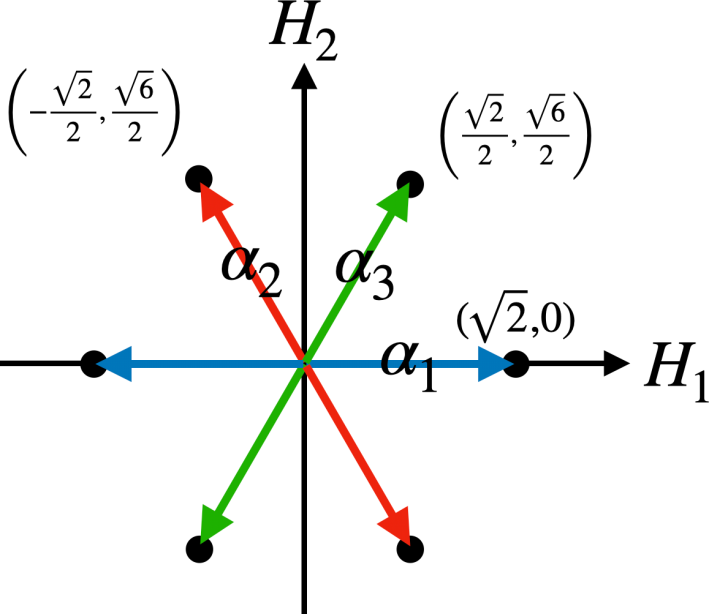
\includegraphics[width=0.3\textwidth]{figs/october/Roots-of-su3-where-a-1-a-2-are-simple-roots.png}
		\caption{The colors represent the actual color charge.}
		\label{fig:roots}
	\end{center}
	\vspace*{-3em}
\end{wrapfigure}

\parhead{SU(3) example} The matter fields in one's gauge theory transform in the
\textbf{fundamental representation} (or in the \textbf{defining representation},
which is the same as the fundamental representation for most groups of interest
to physicists), meaning that the weights of the fundamental representation 
comprise the possible charges of the particles in your theory. For example, in $
SU(3) $, the Cartan subalgebra is comprised of 
\begin{equation*}
	\lambda_3 = \begin{pmatrix}
	1 & 0 & 0 \\ 0 &-1 & 0 \\ 0& 0 & 0
	\end{pmatrix},\quad 
	\lambda_8 = \frac{1}{\sqrt{3}}\begin{pmatrix}
	1 & 0 & 0 \\ 0 &1 & 0 \\ 0& 0 & -2
	\end{pmatrix}
\end{equation*}

Which are two of the Gell-Mann matrices. This Lie algebra has two raising and 
lowering operators, and two elements of the Cartan subalgebra; we thus need 
two numbers to distinguish the weights, one for each element of the subalgebra.  
The matrices above are already diagonalized, so the eigenvectors are just the 
unit vectors $ \left(1,0,0\right), \dots $; we then understand that the two 
numbers labelling the weights are just the eigenvalues of each member of the 
Cartan subalgebra, organized together (and divided by $ 1/2 $ for technical 
reasons). In this case we have that they should be $ (\lambda_{3,ii}, \lambda_{8,ii}) $, 
where $ ii $ denotes the $ i $-th diagonal element:
\begin{equation*}
	(\mu_1, \mu_2) = \left(\frac{1}{2}, \frac{1}{2\sqrt{3}}\right), 
	\; \left(-\frac{1}{2}, \frac{1}{2\sqrt{3}}\right), 
	\; \left(0, - \frac{1}{\sqrt{3}}\right)
\end{equation*}
These are related to each other by the roots (the weights of the adjoint representation)
of which there are six (see \cref{fig:roots}).

\parhead{Constraint on the angles} One can prove that generally for a weight $
\vbg{\upmu} $ and a root $ \vbg{\upalpha} $ \begin{equation*}
	\mathbox{\frac{\vbg{\upmu}\cdot\vbg{\upalpha}}{\vbg{\upalpha}^2}
		\in \frac{1}{2}\Z}
\end{equation*}	
(which also holds for two roots, obviously). This amounts to the statement that
the angle between roots must be 
\begin{itemize}
\itemsep0em
\item Angle of 90 degrees 
\item Angle of 60 or 120 degrees with a length ratio of 1 
\item Angle of 45 or 135 degrees with a length ratio of $ \sqrt{2} $ 
\item Angle of 30 or 150 degrees with a length ratio of $ \sqrt{3} $.
\end{itemize}
In more complicated 
root systems, however, the roots might live in some higher-dimensional space 
(i.e., $ \R^n $ where $ n > 2$), or the roots might not be unit vectors;
nonetheless this condition will still hold. The group of reflections of the 
root system comprises the Weyl group {\color{myred} (Not sure why it needs to 
be the reflections only; usually this does not comprise the whole symmetry 
group of the roots.)}. 

\subsection{Co-roots}
The co-root of a root $ \vbg{\upalpha} $ is 
\begin{equation*}
	\vbg{\upalpha}^\wedge \equiv \frac{2\vbg{\upalpha}}{\vbg{\upalpha}^2}
	\quad 
	\Longrightarrow 
	\quad 
	\vbg{\upalpha}^\wedge \cdot \vbg{\upmu} \in \mathbb{Z}
\end{equation*}
where the right side of the implication can be thought of as a defining 
property of the co-roots. The Dirac quantization condition 
\begin{align*}
	e^{i\mathbf{m}\cdot \vbg{\upmu}} = 1 
\end{align*}
becomes the condition that $ \mathbf{m} \in 2\pi
\Lambda_{\text{co-root}}(\mathfrak{g}) $, where $
\Lambda_{\text{co-root}}(\mathfrak{g}) $ is the lattice spanned by the co-roots 
(known as the Goddard-Nuyts-Olive quantization condition). Here lattice 
is meant in the usual sense of a set of vectors, not a condition on the ordering.  

It's interesting to note that while for $ \text{SU}(N) $ gauge theory 
the 't Hooft lines are in $\Lambda_{\text{co-roots}}(\mathfrak{g}) = 
\Lambda_{\text{roots}}(\mathfrak{g}^\wedge)$, but for $ \text{SU}(N)/\mathbb{Z}_N $
gauge theory the representations are not labelled by the weight lattice 
$ \Lambda_w(\mathfrak{g}) $ but by $ \Lambda_{\text{co-roots}}(\mathfrak{g}) $,
which can be understood as a consequence of  
\begin{equation*}
	\Lambda_w(\mathfrak{g})/\Lambda_{\text{root}}(\mathfrak{g}) = \mathbb{Z}_N
\end{equation*}
(lattices have a group structure so we can take their quotient). 
This means that the 't Hooft lines 
are labelled by $ \Lambda_w(\mathfrak{g}) $.

Actually, it's a general feature of Lie algebras that the center of the Lie 
group is given by the quotient $ \Lambda_w / \Lambda_{\text{root}} $;
see \href{https://math.stackexchange.com/questions/1749386/relations-between-center-fundamental-group-and-coroot-and-weight-lattices-fo}{here} 
for a technical proof. Though this is not too hard to see how this is the case 
by drawing some root lattices overlaid on weight lattices. For instance in SU(2)
we'd have the set of integers for the roots, and the root lattice would be 
the integers and the integers displaced by $ 1/2 $; modding by the root lattice 
then just gives us $ \left\{0, 1/2\right\} \simeq \mathbb{Z}_2$. The argument
follows for $\text{SU}(N)$: see for instance \href{http://jde27.uk/lgla/33_classification_accessible.html}{here}. 
A crucial property is that the root lattice vectors have larger norms than the 
weight lattice vectors so that the quotient is not the trivial group.

\section{Projective Representations, Central Extensions}\label{sec:projective-reps}
Mathematically, the projective representation of a group $ G $ is defined as the group 
homomorphism 
\begin{equation*}
	G \rightarrow \text{GL}(V)/F^\ast
\end{equation*}
where $ \text{GL}(V) $ is the general linear group over some vector space 
$ V $ over a field $ F $, and $F^\ast \vartriangleleft \text{GL}(V) $ is the normal
subgroup consisting of scalar multiples of the identity operator. 

In quantum mechanics we map the group elements to unitary operators on Hilbert 
space, but quotient by operators $ e^{i\phi} \cdot \mathbb{I} = e^{i\phi} $ 
because states are equivalent up to a phase. The allowable 
scalar multiples all have to be of magnitude one since we are working with 
unitary representations, hence they may be written as a phase; hence the 
representation of $ G $ we must work with in quantum mechanics is the projective 
unitary representation 
\begin{equation*}
	G \rightarrow U(\mathcal{H})/e^{i\phi},\quad \phi\in \R.
\end{equation*}

\parhead{Central extension} If we want to move from a projective representation to an ordinary
representation (no modulo by $ F^\ast $), we can promote $ G $ to its universal 
cover $ \tilde{G} $: 
\begin{equation*}
	G \curvearrowright \mathcal{H} \text{ by projective rep.}
	\longrightarrow
	\text{universal cover }\tilde{G} \curvearrowright \mathcal{H}
	\text{ by ordinary rep.}
\end{equation*}
The universal cover $ \tilde{G} $ turns out to be the \textbf{central extension}
of $ \rho^{-1}(F^\ast) $ by $ G $, where $ \rho^{-1}(F^\ast) $ is the preimage of
$ F^\ast $ under the representation $ \rho $. That is, $ G $ is the quotient $
\tilde{G}/\rho^{-1}(F^\ast) $, $ \rho^{-1}(F^\ast) $ is in the center of $
\tilde{G} $, and the following is a short exact sequence: 
\begin{equation*}
	1 \rightarrow \rho^{-1}(F^\ast) \rightarrow \tilde{G} \rightarrow G \rightarrow 1
\end{equation*}
Generally, the central extension of a group $ N $ by $ G $ is some $ \tilde{G} $ such 
that $ N $ is in the center of $ \tilde{G} $ and $ \tilde{G}/N \simeq  G $.
This leads to the statement that the quantum group corresponding to a symmetry 
is the central extension of that symmetry group, for that central extension 
gives you a group of which the projective representation is an ordinary 
representation. 

There is an additional statement to the effect that the second cohomology group 
of a Lie group classifies the central extension, but I do not know algebraic 
topology yet so I haven't a clue what this means. Regardless this does lead to a 
simple way to understand why semi-simple finite dimensional Lie algebras do not 
possess a central charge whereas the Virasoro algebra does. Will return to this 
later!

\parhead{Example} An example is SO(3), which becomes the central
extension/universal cover SU(2). The quantum representation of SO(3) is a 
projective representation, but an ordinary representation of SU(2). 

\section{Short Exact Sequences}
One might see short exact sequences thrown around a ton (see previous section);
reading the Wikipedia/nLab pages doesn't do much to answer why a certain set of
objects forming a short exact sequence is of note. The actual reason is that 
they essentially express, in the most general and unambiguous way, a quotient 
relationship between groups. 

Namely, if $ G/H = N $, then we cannot simply write $ G = H\times N $; in fact, 
it could be the case that $ G = H\ltimes N$ for a semidirect product. The 
short exact sequence, however, expresses this relationship exactly (no pun intended): 
\begin{equation*}
	A \rtimes C \simeq B
	\quad \iff\quad 
	0 \longrightarrow A \xrightarrow{\;\alpha\;}
	B \xrightarrow{\; \beta \;} C \longrightarrow 0
	\quad \iff \quad
	C \simeq B/A
\end{equation*}

If the sequence \textit{splits}, the semidirect product turns into the direct
product: $ A \rtimes C \rightarrow A \times C $. 

We can see that in the case of groups this is in line with the textbook definition: 
the kernel of ... is the image of ....


\section{Semi-Direct Product}
A mnemonic for which of the groups does not possess an induced group composition 
is that the side of $ \ltimes $ with the vertical line points toward the group 
with the induced composition. So the side that looks like the normal direct product 
is the opposite of what you would expect it to be. 

We have that if a system enjoys two symmetries $ A $ and $ B $, and $ A $ 
and $ B $ don't commute, $ G\not\simeq A\times B$, or $ G $ cannot simply be the 
direct product of its two symmetries $ A $ and $ B $. It's easiest to see this 
by proving the contrapositive: 
\begin{equation*}
	G \simeq A \times B \Longrightarrow A \text{ and } B \text{ commute}.
\end{equation*}
which follows easily from the definition of the direct product: if $ a\in A $, 
$ b\in B$, 
\begin{equation*}
	(a, e) \cdot (e, b) = (a, b) = (e, b) \cdot (a, e).
\end{equation*}

We can see by construction that the semidirect product admits a noncommutative 
pair of symmetries like this. Let $ a, e_A\in A $ and $ b, e_B \in B $. Then
for $ A \ltimes B $	we have 
\begin{gather*}
	(a, e_B)\cdot(e_A, b) 
		= (a, e_B \cdot \varphi_{e_A} (b)) = (a, \varphi_{e_A}(b))\\ 
	(e_A, b)\cdot(a, e_B)
		= (a, b\cdot \varphi_a(e_B))
		= (a,b)
\end{gather*}
(Recall that automorphisms, being homomorphisms, must send the identity to itself.)
In general we can choose $ \varphi_{e_A} $ such that $ b\neq \varphi_{e_A} (b)
$. This means that $ a $ and $ b $ don't commute provided we choose our
automorphism appropriately, which is what we would like. 

We can go a step further and make this construction for the symmetry 
enjoyed by the particle on a ring (\cref{sec:particle-on-ring}), 
$ \mathbb{Z}_2 \ltimes \text{U}(1) $
\begin{equation*}
	P T_\alpha P 
		= (P, e ) \cdot (e, T_\alpha) \cdot (P, e)
		= (P, e) \cdot (P, T_\alpha) 
		= (P^2, \varphi_P(T_\alpha))
		= (e, T_{-\alpha})
\end{equation*}
where we have to stipulate $ \varphi_P(T_\alpha) = T_{-\alpha} $. Had we just 
used $ \mathbb{Z}_2 \times \text{U}(1) $ we would find 
\begin{equation*}
	P T_\alpha P 
		= (P, e ) \cdot (e, T_\alpha) \cdot (P, e)
		= (P, e) \cdot (P, T_\alpha) 
		= (e, T_\alpha).
\end{equation*}


\section{Pontryagin Dual}
The Pontryagin dual is occasionally referred to as the generalization of the 
Fourier transform, although this isn't quite right. The correct statement is that 
the Pontryagin dual generalizes the domain of the Fourier transform. Where the 
time domain---also $ \R $---has a dual frequency domain $ \R $ over which the
Fourier transform is defined, or where the crystal lattice has a dual reciprocal
lattice, any locally compact Abelian group $ G $ has a Pontryagin dual $
\widehat{G} $ over which a generalization of the Fourier transform may be
defined. In fact, we can calculate the Pontryagin duals for a selection of spaces 
to prove the following familiar Fourier analysis correspondences: 
\begin{table}[h]
\centering
\begin{tabular}{c c c c}
$ G $ & \textbf{``Time'' domain} & $ \widehat{G} $ & \textbf{``Frequency'' domain}\\ \hline
$ \R $ & (continuous, non-compact) & $\mathbb{R}$ & (continuous, non-compact) \\ 
$ \mathbb{Z} $ & (discrete, non-compact) & $S^1$ &  (continuous, compact) \\ 
$ S^1 $ & (continuous, compact) & $ \mathbb{Z} $ & (discrete, non-compact) \\ 
$ \mathbb{Z}_n $ & (discrete, compact) & $ \mathbb{Z}_n $ & (discrete, compact) \\
\end{tabular}
\end{table}



\section{Axial Current and Anomaly}
I recently did a problem involving an axial (or chiral) anomaly. In some Dirac
fermion theory the Lagrangian has the $ \text{U}(1)_\text{V}\times
\text{U}(1)_\text{A} $ symmetry
\begin{align*}
	\text{Vector current:}\quad \psi(x) \rightarrow e^{i\theta}\psi(x) 
	\qquad &\Longrightarrow \qquad J^\mu = \bar{\psi}(x) \gamma^\mu \psi(x)\\
	\text{Axial current:}\quad \psi(x) \rightarrow e^{i\gamma^5\theta}\psi(x) 
	\qquad &\Longrightarrow \qquad J^\mu = \bar{\psi}(x) 0\gamma^5 \gamma^\mu \psi(x)
\end{align*}
The vector current is associated with charge conservation {\color{myred} [relationship to 
gauge symmetry?]}.  
Let's study this axial conserved current more explicitly. The in Weyl basis:
\begin{align*}
	J^5_\mu = \psi^\dagger \gamma^0 \gamma^5 \gamma^\mu \psi 
\end{align*}
so that
\begin{equation*}
	J^5_k 
		= \begin{bmatrix}
		\psi^\dagger_L & \psi^\dagger_R
		\end{bmatrix}
		\begin{bmatrix}
		0 & 1 \\ 1 & 0
		\end{bmatrix}
		\begin{bmatrix}
		-1 & 0 \\ 0 & 1
		\end{bmatrix}
		\begin{bmatrix}
		0 & \sigma^k \\ -\sigma^k & 0
		\end{bmatrix}
		\begin{bmatrix}
		\psi_L \\ \psi_R
		\end{bmatrix}
		= - \psi_L^\dagger \sigma^k \psi_L  - \psi_R^\dagger \sigma^k \psi_R
		= - J_{\mu = k}
\end{equation*}
where $ J_\mu $ is vector current.
\begin{align*}
	J^5_0 
		= \begin{bmatrix}
		\psi^\dagger_L & \psi^\dagger_R
		\end{bmatrix}
		\begin{bmatrix}
		0 & 1 \\ 1 & 0
		\end{bmatrix}
		\begin{bmatrix}
		-1 & 0 \\ 0 & 1
		\end{bmatrix}
		\begin{bmatrix}
		0 & 1 \\ 1 & 0
		\end{bmatrix}
		\begin{bmatrix}
		\psi_L \\ \psi_R
		\end{bmatrix}
		= \psi_L^\dagger \psi_L - \psi_R^\dagger \psi_R
\end{align*}
In $(1+1)$d (the Schwinger model), we can express the magnitude of this
non-conserved quantity as some scalar field which ends up being the bosonized
field in the bosonization of the Schwinger model.

\parhead{Consequences (chat with Humberto)} I briefly spoke with Humberto 
about the physical consequences of this anomaly. One thing he said is that 
indeed you can think of this type of anomaly as a source term in your Lagrangian, 
so that the field theory is producing fermions of a certain chirality. 
As for how this shows up in experiment, the upshot was that in certain high 
energy processes you find that the incoming and outgoing states do not preserve 
chirality. 

\chapter{November}
\begin{tocbox}
\minitoc
\end{tocbox}

\section{Hubbard-Stratonovich, MFT, etc.}
A few things are said about the relationship between the Hubbard-Stratonovich 
transformation, mean-field theory, and the saddle-point approximation:
\begin{itemize}[nosep]
	\item The saddle-point approximation of the Hubbard-Stratonovich transformation 
		is mean-field theory. 
	\item The saddle-point approximation provides corrections to the mean-field 
		approximations. 
	\item The Hubbard-Stratonovich transformation renders mean-field theory 
		exact.
\end{itemize}

\section{Heisenberg Model and $\text{QED}_\text{3}$}\label{sec:heisenberg-qed3}
The Heisenberg model is not exactly solvable in $ (2+1) $-d, but one can still 
gain insight into the structure of its ground state and excitations by 
pursuing a large-$ N $ approximation in an $ \text{SU}(N) $ version of the
theory. This is achieved through a menagerie of transforms and approximations
which will eventually take us to a solvable $ U(1) $ lattice gauge theory with a
zoo of background gauge fields corresponding to different minima or phases of
the theory. One particular minimum corresponds to a field theory whose continuum
limit is massless $ \text{QED}_3 $. We will also see that this theory will
afford us insight into the ground of state of the actual $ \text{SU}(2) $
Heisenberg model by providing us variational wavefunction ansatze based on the 
exact large-$ N $ phases of the theory.

\subsection{Gauge Fields via Hubbard-Stratonovich}
Starting from the fact that the Heisenberg interaction can be written 
\begin{equation*}
	\mathbf{S}_i \cdot \mathbf{S}_j 
		= \frac{1}{2}c^{\dagger}_{\alpha i} c_{\beta i}
			c_{\beta j}^\dagger c_{\alpha j}
				- \frac{1}{4}n_i n_j
\end{equation*}
(the repeated greek indices sum over spin components) with half-filling 
the fermion number term becomes a constant so that the $ \text{SU}(2) $
Heisenberg Hamiltonian is simply 
\begin{equation*}
	H = \frac{J}{2}\sum_{\langle i,j \rangle}
		c_{\alpha i}^\dagger c_{\beta i} c_{\beta j}^\dagger c_{\alpha i}
\end{equation*}

To perform a Hubbard-Stratonovich transformation it is necessary to work in the
path integral representation and thus we Legendre transform to find the 
Lagrangian
\begin{equation*}
	\mathcal{L}
		= i\sum_i c_{\alpha i}^\dagger(t) \partial_t c_{\alpha i}(t)
			+ \sum_i \varphi_i(t) (c_{\alpha i}^\dagger (t) c_{\alpha i}(t) - 1)
				- H
\end{equation*}
where we have introduced the background field $ \varphi_i(t) $ as a Lagrange 
multiplier enforcing the half-filling. The presence of this field will turn 
out to be crucial to our understand of this as a relativistic gauge theory. 

\begin{alertbox}[Aside]
Fields without a kinetic term appearing in a path integral become Lagrange 
multipliers enforcing a constraint. This can be seen from the fact that 
in the Euler-Lagrange equation
\begin{equation*}
	\frac{\partial\mathcal{L}}{\partial \phi} - \partial_\mu \frac{\partial
	\mathcal{L}}{\partial(\partial_\mu \phi)} = 0
\end{equation*}
the second term in the LHS vanishes and so the field's equation of motion 
becomes an \textit{algebraic} (contrast \textit{differential}) equation
for a constant $ \phi $. Note that this does mean the Lagrange multiplier 
does not experience quantum fluctuations. 
\end{alertbox}
				
Now proceeding with the Hubbard--Stratonovich transformation, we are able to 
convert a quartic interaction into an auxiliary field--$\text{fermion}^2$ interaction 
and an auxiliary field quadratic interaction. The auxiliary field we 
introduce is a complex bosonic link variable $ \chi_{ij} = \rho_{ij}(t) e^{iA_{ij}(t)} = \chi_{ji}^\ast$; 
where we anticipated its analogy with $ U(1) $ lattice gauge theory by
expressing it as an amplitude $ \rho $ and phase $ A $. The Lagrangian is then
\begin{align}\label{eq:lagrangian-chi}
	\mathcal{L}
		&=i\sum_i c_{\alpha i}^\dagger(t) \partial_t c_{\alpha i}(t)
			+ \sum_i \varphi_i(t) (c_{\alpha i}^\dagger (t) c_{\alpha i}(t) - 1)\\
				&\qquad - \frac{2}{J}\sum_{\langle i,j \rangle} |\chi_{ij}|^2
				+ \sum_{\langle ij \rangle} \left(
					c_{\alpha i}^\dagger(t) \chi_{ij} (t) c_{\alpha j} (t) 
					+ c_{\alpha j}^\dagger (t)\chi_{ij}^\ast(t) c_{\alpha i}(t)
				\right)\nonumber
\end{align}
where we've had to introduce $ \chi $ and $ \chi^\ast $ to account for the 
presence of two spin-indices in the interaction term. Now, even before the 
Hubbard--Stratonovich transformation the theory has a gauge symmetry in the 
form of $ c_{\alpha i} \rightarrow e^{i\theta_i (t)} c_{\alpha i} $
corresponding to local fermion number conservation. Upon introducing 
gauge fields we see they transform as
\begin{gather*}
	\chi_{ij}(t) \rightarrow e^{-(\theta_j(t) - \theta_i(t))}\chi_{ij}(t),\quad 
	\varphi(t)_i \rightarrow \varphi_i (t) + \partial_t \theta_i(t)\\ 
	A_{ij}(t) \rightarrow  A_{ij} + \Delta_{ij} \theta_i(t),\quad \Delta_{ij}\equiv\text{lattice derivative}
\end{gather*}
It is not hard to see that these are the gauge transformations of a $ \text{U}(1) $
gauge theory; in particular, we find that $ \chi_{ij} $ serves the role of a 
link variable or Wilson line with the Abelian linear gauge transformation 
\begin{equation*}
	\chi_{ij}(t) =\rho_{ij}e^{iA_{ij}(t)}\quad \Longrightarrow \quad 
	e^{A_{ij}(t)} \rightarrow G_i(t) e^{A_{ij}(t)} G_j(t)^{-1}
\end{equation*}
(see, e.g., Rothe, \textit{Lattice Gauge Theories}), so that the fields $ (A,\varphi) $
together make $ A_{\mu, i}(t) $ with timelike component $ \varphi $. Note, 
however, that the Lagrangian is not fully gauge invariant under this 
transformation: the first two terms of \cref{eq:lagrangian-chi} transform as 
\begin{align*}
	& i c^{\dagger}_{i\alpha}e^{-i\theta_i} \partial_t (e^{i\theta_i} c_{i\alpha})
		+ [\varphi_i + \partial_t \theta_i] (c^{\dagger}_{\alpha i} c_{\alpha i} - 1)\\
	&\qquad = 
		ic^\dagger_{\alpha i}\partial_t c_{\alpha i}
		+\varphi_i (c^\dagger_{\alpha i}c_{\alpha i} - 1)
			 - c^\dagger_{\alpha i} c_{\alpha i} \partial_t \theta_i 
			 + \partial_t\theta_i c_{\alpha i}^\dagger c_{\alpha i} 
			+ \partial_t \theta_i\\
	&\qquad = 
		ic^\dagger_{\alpha i}\partial_t c_{\alpha i}
		+\varphi_i (c^\dagger_{\alpha i}c_{\alpha i} - 1)
			+ \partial_t \theta_i
\end{align*}
And we find there is a hanging $ \partial_t \theta_i $ term. The culprit 
is the $ -\varphi_i $ term in the original Lagrangian; fortunately, it is 
not hard to find the proper constraint on $ \phi $ such that gauge invariance 
is restored. We simply note that its amplitude is 
\begin{equation*}
	\exp\left(i\int dt \sum_i \varphi_i(t)\right) 
		= \prod_i \exp \left(i\int dt \;\varphi_i(t)\right)
		= \prod_i \exp \left(i\int\; dt A_{0i}(t) \right)
\end{equation*}
and that for periodic boundary conditions in time, we can construct a timelike 
Wilson loop along a path $ \Gamma_i $ closing around the spacetime manifold,
which transforms under gauge transformations as
\begin{equation*}
	\prod_i \exp\left(i\int_{\Gamma_i} dx^\mu A_{\mu i}\right)
		\quad \rightarrow \quad 
	\prod_i \left(i\exp\left(\int_{\Gamma_i} dx^\mu A_{\mu i}\right)
	 + \exp\left(i\int_\Gamma dx^\mu \theta_{\mu i}\right)
	 \right)
\end{equation*}
Using Stokes' theorem, we find that provided the form $ d\theta $ is closed, 
gauge invariance is restored. Note, however, that the action itself is not 
invariant under large gauge transformations, which leave the amplitude invariant 
but wind around from $ 0 $ to $ 2\pi k $, $ k\in \mathbb{Z} $ such that 
the action gains an additional factor $ 2\pi k $; this suggests the term acts
as a sort of Chern-Simons term for this theory. For the effective action we will
later derive to be consistent with the half-fililng constraint, one must keep
track of this term, as the saddle point of the temporal component $ \delta
S_{\text{eff}} /\delta A_0 $ should recover the constraint. In what follows,
however, we only consider the saddle point of the spatial components of the 
gauge fields, and we ignore the term for the remainder of the discussion.
This is justified by the fact that in the $ \text{SU}(N) $ theory with $
S_{\text{eff}} = N\int \mathcal{L} $this term is of order $ 1/N $ and the
half-filling constraint is irrelevant as $ N \rightarrow \infty $. 

\subsection{Large \textit{N} and Saddle-Points}
Our Hubbard-Stratonovich transformation has then turned this Heisenberg model
into a $ \text{U}(1) $ gauge theory with a Abelian gauge field without a
dynamical term $ F^{\mu\nu} $ and with a fluctuating magnitude $ \rho $. In the
saddle point approximation, we will find that the fluctuations in $ \phi $ and $
\chi $ are suppressed and they play the role of background fields by taking on
classical minima of an effective action. This will produce a mean-field
Hamiltonian that is nothing more than a tight-binding model with non-uniform
hopping parameter, and which we will be able to solve for different classical
gauge field configurations. This saddle point approximation is justified by
making a large-$N$ approximation which renders the mean field theory exact when
$ N \rightarrow \infty $; such an approximation provides $ 1/N $ as a parameter 
about which to organize perturbative corrections. 

To employ this approximation we generalize to an $ \text{SU}(N) $ Heisenberg 
model and choose a group representation such that the theory describes $ N $ 
different fermion species or ``flavors,'' and each site is populated by $ N/2 $
fermions (other representations are possible, most notably that of Read and
Sachdev). The fermion operator algebra is then indexed 
by flavor $ a $ in addition to spin $ \alpha $---$ c_{a\alpha} $. The Hubbard-Stratonovich 
transformation also supplies the gauge fields with these flavor indices, and 
the $N/2$-filling constraint is modified to $ c_{\alpha a}^\dagger c_{\alpha b}
= \delta_{ab} N/2 $ such that the $ \text{SU}(N) $ Lagrangian is 
\begin{align}
	\mathcal{L}
		&=i\sum_i c_{\alpha a, i}^\dagger(t) \partial_t c_{\alpha a, i}(t)
			+ \sum_i \varphi_{ab,i}(t) 
				(c_{\alpha a, i}^\dagger (t) c_{\alpha b, i}(t) - \delta_{ab}\tfrac{N}{2})\\
				&\qquad - \frac{N}{J}\sum_{\langle i,j \rangle} |\chi_{ab,ij}|^2
				+ \sum_{\langle ij \rangle} \left(
					c_{\alpha a, i}^\dagger(t) \chi_{ab,ij} (t) c_{\alpha b, j} (t) 
					+ c_{\alpha b,j}^\dagger (t)\chi_{ab,ij}^\ast(t) c_{\alpha a, i}(t)
				\right)\nonumber
\end{align}
where here we think of $ \chi_{ab} $ as a complex matrix on each of the links 
of the lattice, signalling that this is now a non-Abelian gauge theory with 
Yang-Mills fields $ A^{ab}_{ij}(t) $.
To find the saddle point of $ \chi $ and $ \varphi $ we must first integrate out 
the fermions; as the Hubbard-Stratonovich transformation renders the Lagrangian 
quadratic $ c_{\alpha a} $, the integral is Gaussian and reduces to a functional 
determinant (temporarily suppressing spin indices): 
\begin{equation*}
	\det\left(-i \partial_t \delta_{ab} + \varphi_{ab, i}(t) + \chi_{ab,ij} (t)
		+ \chi_{ij,ab}(t)^\ast  \right)
\end{equation*}
The identity $ \det A = \exp(\tr \ln A) $ lets us reinsert these terms into the 
Lagrangian to obtain an effective action: 
\begin{align}\label{eq:s-eff}
	S_{\text{eff}}
		&=
		-i 2 N\tr \ln \left(i \partial_t \delta_{ab} + \varphi_{ab, i}(t) + \chi_{ab,ij} (t)
		+ \chi_{ij,ab}(t)^\ast  \right) - \frac{N}{J}\int dt\sum_{\langle i,j \rangle} |\chi_{ab,ij}|^2
\end{align}
where the factor of $ 2N $ comes from the spin indices and the trace is understood
to integrate over time and space. That this Lagrangian has an overall factor 
of $ N $ is crucial for the saddle point to become exact when $ N \rightarrow \infty $, 
at least from a mathematical standpoint. 

The physical grounds on which the large-$ N $ approximation is understood to
render the saddle-point approximation exact as follows: A valence bond between 
two sites is annihilated (created) by the operator $ c_{\alpha i}^{(\dagger)}
c_{\alpha j}^{(\dagger)}$ (in the $ \text{SU}(N) $ case actually $ N $ such
valence bonds between the different species are created); 
the Heisenberg Hamiltonian is then nothing more a sum over valence bond number
operators:
\begin{equation*}
	H = -\frac{J}{N}\sum_{\langle i,j \rangle}\left(c_{\alpha i}^\dagger
	c_{\alpha j}^\dagger\right)
	\left(c_{\beta i}c_{\beta j}\right)
\end{equation*}
such that when one such local term acts on a valence bond, the bond is preserved
and we obtain an eigenenergy $ -J $: $ H \ket{\text{bond}} = -J
\ket{\text{bond}}$. When the Hamiltonian acts on a link without a bond, it 
creates one bond at that link, and annihilates two bonds terminating at the
link---each of which is one among $ N/2 $ possible choices---and creates
bonds between the two newly unbonded sites. The Hamiltonian produces an equal-weight
superposition over all possible ways to do this, each of which possesses an
amplitude $ -J/N $. Indeed, there $ N $ possible ways of doing this, 
so that the probability of such a process is actually $ O(1) $ in aggregate;
nevertheless, only one bond is annihilated at a time, so that the fluctuations
are $ O(1/n) $ and the bond number operator takes on a classical value as $ n
\rightarrow \infty $. 

\subsection{Solving the Mean Field Hamiltonian}
In fact, when the saddle-point approximation is exact, we can read off of 
\cref{eq:lagrangian-chi} a corresponding exact mean-field tight-binding-like
Hamiltonian: 
\begin{equation}\label{eq:h-mf}
	H_{\text{MF}}
	= \sum_{ij}c_{\alpha i}^\dagger \chi_{ij} c_{\alpha j}
				+ c_{\alpha j}^\dagger \chi_{ij}^\ast c_{\alpha i}
\end{equation}
Here we've suppressed the flavor index and dropped the constant term $
|\chi_{ij}|^2 $. In order to find the actual classical values of $ \chi_{ij} $
we must extremize the action by finding the saddle point; we now turn to this 
task. 

A saddle point corresponds to a configurations of $ \chi $, or, more
precisely, $ \rho $ and $ A $, such that the action in \cref{eq:s-eff} is 
stationary:
\begin{equation*}
	\frac{\delta S_{\text{eff}}}{\delta \rho_{ij}} = 0 ,\quad 
	\frac{\delta S_{\text{eff}}}{\delta A_{ij}} = 0 ,\quad 
\end{equation*}
Two further constraints reduce the ansatze we must consider: (1) Elitzur's
theorem informs us that only gauge invariant operators carry non-vanishing
expectation values, meaning that different saddle points must correspond to 
different expectation values of some gauge invariant parameter. The natural 
operator to choose is the plaquette loop $ W(\square) = e^{i\Phi} = \prod_\square 
e^{iA_{ij}}$ with flux $ \Phi = \sum_\square A_{ij}(t)$. (2) By stipulating that 
$ \chi_{ij}(t) $ should be in an equilibrium configuration, i.e., it is
time-reversal invariant, we place additional constraints on the flux of the theory. 
In particular, since the time-reversal operator $ \mathsf{T} $ has the effect 
\begin{equation*}
	\mathsf{T} e^{iA} \mathsf{T}^{-1} 
		= e^{-iA},
\end{equation*}
it must take $ \Phi $ to $ \sum_\square - A_{ij}(t) = -\Phi $, and the requirement 
that this describe an equilibrium distribution limits the ansatze to those 
with flux $ \Phi = 0 $ \textit{or} $ \Phi = \pi $ (since $ A_{ij} $ is defined up 
to integer multiples $ 2\pi $, we have $- \Phi = -\pi \sim -\pi + 2\pi = \pi =
\Phi$). As it turns out, we may choose saddle-point ansatze with constant $
\rho_{ij} $ and $ A_{ij} = 0,\pi $, and those choices correspond to two
different phases of this model. Shortly, we will specialize to $ \Phi = \pi $,
the so-called $ \pi $-flux phase. However, we first return to \cref{eq:h-mf} to
find its spectrum for
\begin{equation*}
	\chi_{ij} = \begin{cases}
		\chi_x \exp(-i\Phi/4) & \text{horizontal link}\\
		\chi_y \exp(-i\Phi/4) & \text{vertical link}
	\end{cases}
\end{equation*}
this ensures that the flux through a plaquette is $ \Phi $ and the bond variables 
are constant throughout the lattice. \Cref{eq:h-mf} is then 
\begin{equation*}
	H_{\text{MF}} = \sum_{\langle ij\rangle}
	c_{\alpha i}^\dagger \chi_{x,y} e^{i\Phi} c_j + c_j^\dagger \chi_{x,y}e^{-i\Phi} c_i
\end{equation*}
whhere $ \chi_{x,y} $ denotes $ \chi_x $ or $ \chi_y $ depending on the link 
$ \langle i j\rangle $. The usual technique is to Fourier transform to 
$ c_{\alpha k} $ operators; before doing this, however, the trick is to 
introduce a local $ 2\times 2 $ Hamiltonian in the spirit of a Nambu spinor 
diagonalization. In what follows we specialize to bipartite lattices; in
particular, we notice that the sum over links $ \langle i, j\rangle $ will
always contain one index in an odd sublattice and one index in an even
sublattice. Then we write 
\begin{equation*}
	H_{\text{MF}}
		= \sum_{\langle ij \rangle}
			\begin{bmatrix}
			c_i \\ c_j
			\end{bmatrix}^\dagger 
			\begin{bmatrix}
			0 & \chi_{x,y} e^{-i\Phi/4}\\
			\chi_{x,y} e^{i\Phi/4} & 0 
			\end{bmatrix} 
			\begin{bmatrix}
			c_i \\ c_j
			\end{bmatrix}
\end{equation*}
where $ i $ is always in an odd sublattice and $ j $ is always in an 
even sublattice. It is easy to diagonalize this matrix and find 
\begin{equation}\label{eq:heisenberg-qed3-hmft}
	H_{\text{MF}}
		= \sum_{\langle ij \rangle}
			\begin{bmatrix}
			c_i \\ c_j
			\end{bmatrix}^\dagger 
			\begin{bmatrix}
			e^{i\Phi/4} & e^{i\Phi/4}\\ 
			e^{-i\Phi/4} & -e^{-i\Phi/4}
			\end{bmatrix}^\dagger
			\begin{bmatrix}
			\chi_{x,y} & 0 \\ 0 & -\chi_{x,y}
			\end{bmatrix}
			\begin{bmatrix}
			e^{i\Phi/4} & e^{i\Phi/4}\\ 
			e^{-i\Phi/4} & -e^{-i\Phi/4}
			\end{bmatrix}
			\begin{bmatrix}
			c_i \\ c_j
			\end{bmatrix}
\end{equation}
Now we are ready to Fourier transform. Consider first nearest neighbor
interactions along a horizontal link: $ \mathbf{x} $ and $ \mathbf{x}' =
\mathbf{x} + (1,0) $, such that $ \mathbf{k}\cdot \mathbf{x}' =
\mathbf{k}\cdot\mathbf{x} + k_x $. Such a term Fourier transforms as 
\begin{equation*}
	\sum_{\mathbf{x}, \mathbf{x}'}c_\mathbf{x}^\dagger c_\mathbf{x'}^\dagger
	\rightarrow 
		c_\mathbf{k}^\dagger c_{\mathbf{k}'}
		e^{-i (\mathbf{k}-\mathbf{k}') \mathbf{x}} e^{ik_x}
\end{equation*}
since the sums over vertical and horizontal nearest neighbor sites is disjoint, 
considering the vertical links just induces a new term $ \exp(ik_y) $:
\begin{equation*}
	\sum_{\langle \mathbf{x_1} \mathbf{x_2}\rangle}c_\mathbf{x}^\dagger c_\mathbf{x'}^\dagger
	\rightarrow 
	\sum_{\mathbf{k}} 
	c_\mathbf{k}^\dagger c_{\mathbf{k}'}
	e^{-i (\mathbf{k}-\mathbf{k}') \mathbf{x}} (e^{ik_x} + e^{{ik_y}}).
\end{equation*}
where the $ \exp(-i(\mathbf{k} - \mathbf{k}')) $ turns into $ \delta(\mathbf{k}
- \mathbf{k}') $ upon resolving the spatial sum.
\begin{figure}[t]
	\centering
	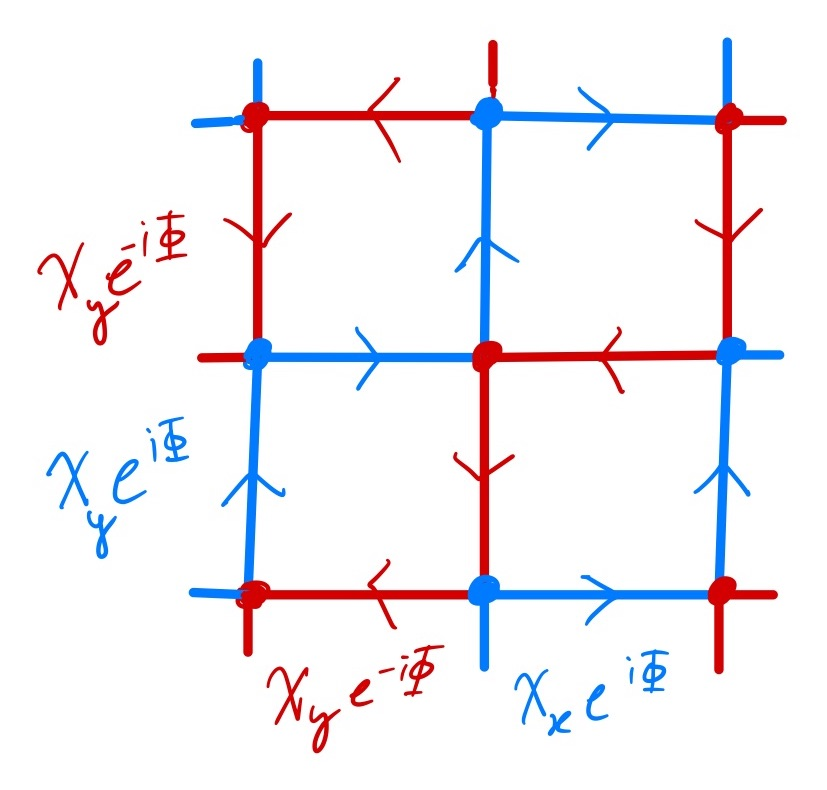
\includegraphics[width=0.3\textwidth]{figs/november/bipartite-gauge.jpg}
	\caption{}
	\label{fig:heisenberg-qed3-bipartite}
\end{figure}

Also note that in this bipartition of $ \chi $, every $ i $ index is associated 
with a horizontal $\chi_x $ bond but a vertical $ \chi_y^\ast $ bond (see 
\cref{fig:heisenberg-qed3-bipartite}). This means that when we combine the 
vertical and horizontal links in \cref{eq:heisenberg-qed3-hmft} we find that they
contribute terms $ \chi_{y}^\ast \exp(ik_y) $ and links $ \chi_x \exp(ik_x) $
respectively. \Cref{eq:heisenberg-qed3-hmft} then becomes 
\begin{align*}
	H_{\text{MF}}
		= \sum_{\langle k \rangle}
		(\cdots)
			% \begin{bmatrix}
			% c_i \\ c_j
			% \end{bmatrix}^\dagger 
			% \begin{bmatrix}
			% e^{i\Phi/4} & e^{i\Phi/4}\\ 
			% 1 & -1 
			% \end{bmatrix}^\dagger
			\begin{bmatrix}
				1 & 0 \\ 0 & -1
			\end{bmatrix}&
			\bigg(
				\begin{bmatrix}
				e^{i\Phi/4} & e^{i\Phi/4}\\ 
				e^{-i\Phi/4} & - e^{-i\Phi/4}
				\end{bmatrix}
				\begin{bmatrix}
					c_k \chi_x
					e^{ik_x}\\
					c_k\chi_x
					e^{-ik_x}
				\end{bmatrix}\\
				&\qquad 
				+ 
				\begin{bmatrix}
				e^{-i\Phi/4} & e^{-i\Phi/4}\\ 
				e^{i\Phi/4} & -e^{i\Phi/4}
				\end{bmatrix}
				\begin{bmatrix}
					c_k \chi_y
					e^{ik_y} \\
					c_k \chi_y
					e^{-ik_y}
				\end{bmatrix}
			\bigg)
\end{align*}
By combining the latter two factors we find that the excitations diagonalizing 
this system are 
\begin{align*}
	\text{Odd sites:} \qquad c_o = \left(e^{i\Phi/4}\chi_x \cos k_x + e^{-i\Phi/4} \chi_y \cos k_y \right)
		e^{i \mathbf{k}\cdot \mathbf{x}}\\
	\text{Even sites:} \qquad c_e = \left(e^{-i\Phi/4}\chi_x \cos k_x + e^{i\Phi/4} \chi_y \cos k_y \right)
		e^{i \mathbf{k}\cdot \mathbf{x}}
\end{align*}
where in the even excitations we have made the shift $ \mathbf{k} \rightarrow \mathbf{k} 
+ (\pi/2,\pi/2)$ which is permitted by the perfect nesting of the Fermi surface 
(thereby taking $ \sin k_{xy} \rightarrow \cos k_{xy} $). 
By noticing that the factor in the even sites is the conjugate of the factor 
of the odd sites, we can pull out the even-site factor at the
meaningless cost of an overall phase and find that 
\begin{equation}
	\text{Odd sites:} \qquad c_o  =\frac{g}{\sqrt{gg^\ast}} e^{i \mathbf{k}\cdot \mathbf{x}},
	\qquad \text{Even sites:} \qquad c_e e^{i \mathbf{k}\cdot \mathbf{x}}
	\label{eq:heisenberg-qed3-excitations}
\end{equation}
with 
\begin{equation*}
	g = e^{i\Phi/4}\chi_x \cos k_x + e^{-i\Phi/4} \chi_y \cos k_y 
\end{equation*}
The presence of two types of excitations represents the doubling of the unit cell
and is reflected in a two-branch spectrum corresponding to the $ \pm 1$
eigenvalues of the Nambu local Hamiltonian. 

The $ \pi $-flux phase in particular has $ \Phi = \pi $ and the spectrum is 
\begin{equation*}
	E(\mathbf{k}) =\pm 2 |\chi| \left(\cos^2 k_x + \cos^2k_y\right)^{1/2}
\end{equation*}
There are four Fermi points\footnote{Note however that because of the perfect
nesting of the Fermi surface only two of those Fermi points are inequivalent.} $
\mathbf{k} = (\pm \pi/ 2,\pm \pi/2) $, near which we can use $ \cos(\pi/2 +
\epsilon) \approx \epsilon$ to approximate
\begin{equation*}
	E(\mathbf{k})\approx 
	\left(
		k_x^2 + k_y^2
	\right)^{1/2}
\end{equation*}
meaning that the dispersion is linear near the gap, the first signature of a 
low-energy effective theory corresponiding to a massless relativistic QFT and 
a Dirac cone. We now explicitly demonstrate this fact.

We first gauge transform to $ \chi_x = |\chi| e^{i\pi/2}=i|\chi| $ and 
$ \chi_y = |\chi|  $ (notice the plaquette flux is still $ \pi $). The 
Hamiltonian of \cref{eq:heisenberg-qed3-hmft} now reads 
\begin{equation*}
	H_{\text{MF}}
		= |\chi| \sum_{\mathbf{r}\in \text{odd}}
		c_\mathbf{r}^\dagger [i(c_{\mathbf{r}-\hat{\mathbf{x}}} 
			+ c_{\mathbf{r} + \hat{\mathbf{x}}})
			+ 
		(c_{\mathbf{r}-\hat{\mathbf{y}}} 
			+ c_{\mathbf{r} + \hat{\mathbf{y}}})] + \text{H.c.}
\end{equation*}
where we've explicitly combined all of the links associated with the odd 
bipartition of the lattice into the summand so that we run over $ \mathbf{r} $
in the odd sublattice.
Now Fourier transforming with \cref{eq:heisenberg-qed3-excitations} and
considering a large system size such that the spectrum becomes continuous, 
we have 
\begin{equation*}
	2|\chi| \int\frac{d^2 k}{(2\pi)^2}
		\left(i\cos k_x + \cos k_y\right) c_e^\dagger(\mathbf{k}) c_o
		(\mathbf{k}) + \text{H.c.}
\end{equation*}
where as usual the cosines come from relative displacements in the 
Fourier factor $ e^{i (x + 1) k_x} $. We can consider a continuum theory 
by limiting ourselves to small wavevectors such that the system does not 
see the Brillouin zone. To do so we shift to momenta $ \mathbf{k} \rightarrow
\mathbf{k} + (\pi/2, \pm\pi/2)$ corresponding to two inequivalent Fermi points
(producing what is sometimes referred to as Fermion doubling) and find 
\begin{equation*}
	-2|\chi|\int\frac{d^2 k}{(2\pi)^2}
		\left(i k_x + k_y\right) c_{1e}^\dagger(\mathbf{k}) c_{1o}
		(\mathbf{k}) + \text{H.c.}
		+ 
		\left(i k_x - k_y\right) c_{1e}^\dagger(\mathbf{k}) c_{2o}
		(\mathbf{k}) + \text{H.c.}
\end{equation*}
We turn our attention to the first Fermi point alone, the $ c_{(o,e)1}  $ 
excitations. We find that the terms can be written in matrix form 
\begin{align*}
	& \left(i k_x + k_y\right) c_{1e}^\dagger(\mathbf{k}) c_{1o}
	(\mathbf{k}) +
	\left(-i k_x + k_y\right) c_{1o}^\dagger(\mathbf{k}) c_{1e}
	(\mathbf{k}) \\
	&\qquad = k_x 
	\begin{bmatrix}
	c_{e1}\\ c_{o1}
	\end{bmatrix}^\dagger
	\begin{bmatrix}
	0 & i \\ -i & 0
	\end{bmatrix}
	\begin{bmatrix}
	c_{e1}\\ c_{o1}
	\end{bmatrix}
	+
	k_y
	\begin{bmatrix}
	c_{e1}\\ c_{o1}
	\end{bmatrix}^\dagger
	\begin{bmatrix}
	0 & 1 \\ 1 & 0
	\end{bmatrix}
	\begin{bmatrix}
	c_{e1}\\ c_{o1}
	\end{bmatrix}\\ 
	&\qquad 
	= -k_x \psi^\dagger_1 \sigma_2 \psi + k_y \psi^\dagger_1 \sigma_1 \psi\\
	&\qquad 
	= -\psi^\dagger_1 \sigma_2\partial_1 \psi + \psi^\dagger_1 \sigma_1\partial_2 \psi
	\equiv \mathcal{H}_1/ 2|\chi|\qquad \text{(Hamiltonian density)}
\end{align*}
where we've introduced the Dirac spinors $ \psi_1 = (c_{e1}, c_{o1}) $,
substituted the Pauli matricesm, and Fourier transformed in the final
step. We've also anticipated the Lorentz covariant form of the Lagrangian 
density by using relativistic indices $ x \rightarrow 1 $, $ y \rightarrow 2 $.
Legendre transforming these terms introduces a new term 
\begin{equation*}
	\mathcal{L}_1 = i\psi_1 \partial_0 \psi_1 
		+ 2|\chi|i\psi_1^\dagger(-\sigma_2 \partial_1 + \sigma_1 \partial_2)\psi_1
\end{equation*}
Using the fact that $ -\sigma_2 = i\sigma_2 \sigma_1 $ and $ \sigma_1 = i\sigma_3\sigma_1 $,
and $ \sigma_3^2 = 1 $
\begin{equation*}
	\mathcal{L}_1 = i \psi_1 \sigma_3 \sigma_3\partial_0 \psi_1 
		+ 2|\chi|i\psi_1^\dagger(i\sigma_3\sigma_1 \partial_1 + i\sigma_3\sigma_2 \partial_2)\psi_1
\end{equation*}
Now we notice that the $ (2+1) $d representation of the Clifford algebra is 
given by $ \gamma_\mu = (i\sigma_3, \sigma_1, \sigma_2) $, so that idenfifying 
$ 2|\chi| $ as the speed of ``light,'' we find 
\begin{equation*}
	\mathcal{L}_1 = i\bar{\psi}_1 \gamma^\mu \partial_\mu \psi_1,\qquad 
	\bar{\psi} = \psi^\dagger \gamma^0.
\end{equation*}
The analysis is identical for the second Fermi point, so we find that the 
Lagrangian density is the sum over the two fermions (indexed by $ a $): 
\begin{equation*}
	\mathcal{L}= i\bar{\psi}_a \gamma^\mu \partial_\mu \psi_a. 
\end{equation*}
It turns out that if one includes fluctuations about the saddle point of 
$ \chi $, we indeed obtain 
\begin{equation*}
	\mathcal{L} = i\bar{\psi}_a \gamma^\mu D_{\mu} \psi_a ,\qquad 
	D^\mu =\partial^\mu +igA^\mu,
\end{equation*}
the Lagrangian of a $ (2+1) $d massless $ \text{U}(1) $ gauge theory. 

\subsection{Concluding Remarks}
By considering an unphysical $ \text{SU}(N)$ generalization of the Heisenberg
model, we have derived a mean-field Hamiltonian \cref{eq:heisenberg-qed3-hmft}
containing a classical background gauge field manifesting as complex, non-uniform 
hopping parameters $ \chi_{ij} $, sometimes referred to as \textit{parton
construction}. To make contact with the actual $ \text{SU}(2) $ Heisenberg
antiferromagnet, one must explicitly reintroduce the single-occupancy constaint
by way of a Gutzwiller projection of the $ c_{(o,e), \mathbf{k}} $ excitations. 
In particular, we construct a Slater determinant of such excitations, 
$ \ket{\psi_\text{free}} $, and fully project out double occupancy: 
\begin{equation*}
	\ket{\psi} = \Pi_i (1-n_{i\uparrow}n_{i\downarrow})\ket{\psi_{\text{free}}}
\end{equation*}
We may then treat the $ \pi $-flux 
phase wavefunction as a variational ansatz with which to explore the ground state 
of the $ \text{SU}(2) $ Heisenberg model.

\subsection*{References}
\begin{itemize}[nosep]
\item Rothe, \textit{Lattice Gauge Theories}. 
\item Fradkin, \textit{Field Theories of Condensed Matter}. See in particular 
	\S 8.4.
\item Marston, Affleck, \textit{Large-n limit of the Hubbard-Heisenberg Model}, 
	[\href{https://journals.aps.org/prb/abstract/10.1103/PhysRevB.39.11538}{PhysRevB.39.11538}].
\item Sachdev, Read, \textit{Large-N expansion for frustrated quantum antiferromagnets},
	[\href{https://journals.aps.org/prl/abstract/10.1103/PhysRevLett.66.1773}{PhysRevLett.66.1773}].
\end{itemize}

\section{Gauge Theories from SSB}

\section{'t Hooft Anomaly: Particle on $\text{S}^\text{1}$}\label{sec:particle-on-ring}
t' Hooft anomalies are often described as ``obstructions to gauging a global
symmetry.'' One illustration Humberto gave is a theory with a $
\text{U}(1)_\text{A} \times \text{U}(1)_{\text{V}} $ symmetry wherein you cannot
gauge $ \text{U}(1)_{\text{A}} $ without rendering $ \text{U}(1)_{\text{V}} $
anomalous and vice-versa. In quantum mechanics (in field theory the story is a 
bit different) the description of 't Hooft anomalies can be given in terms of 
what we learned in \S \ref{sec:projective-reps}: if we cannot rescale the 
action of the (global) symmetry operator on the state so as to make it a linear representation, 
that is, if it is \textit{strictly} a projective representation, we say that 
the symmetry has an 't Hooft anomaly. This is considered an ``obstruction to 
gauging'' because the gauge symmetry of quantum mechanics is the overlabelling 
of Hilbert space up to a phase; if we can't get rid of that phase, there is 
an obstruction. This obstruction manifests itself as a physical inequivalence 
between states that are related by such a phase. Shao claims that this is 
so general a phenomenon as to encompass the fact that qubits are in the 
projective representation of SO(3): qubits are 't Hooft anomalous!?

\parhead{Particle on a ring} Here we illustrate the phenomenon with a supposedly
representative $ (0+1) $-d example, a particle on a ring with a theta term:
\begin{equation*}
	\mathcal{L} = \frac{m}{2}\dot{x}(t)^2 + \frac{\theta}{2\pi}\dot{x}(t)
	\quad \xrightarrow{t = i\tau}\quad 
	\mathcal{L} = \frac{m}{2}\dot{x}(\tau)^2 - \frac{i\theta}{2\pi}\dot{x}(\tau)
\end{equation*}
The theta term is indeed topological. Additionally, being a total derivative, 
it has no effect on the classical equations of motion (see \S\ref{sec:total-derivatives}).
Periodic boundary conditions amount to $ x \simeq x+ 2\pi$, and additionally $
\theta \simeq \theta + 2\pi $. This $ \theta $-periodicity is not postulated, 
but rather a consequence of the invariance of the path integral with respect to 
$ \theta \rightarrow \theta + 2\pi $. Two quick ways of seeing this, from Tong: 
\begin{itemize}[itemsep=0.2em]
\item The Euclidean partition function will have a total derivative term 
	which captures instanton effects by yielding a topological charge $ k $
	corresponding to the winding number.
	\begin{equation*}
			i\frac{\theta}{2\pi}
		\int_0^\beta d\tau\;	\partial_\tau x = i\frac{\theta}{2\pi} 2\pi k
		= i\theta k
	\end{equation*}
	(the $ i $ comes from $ t = i\tau $). Put more crudely, this we have 
	that the integral over $ \partial_\tau x $ must be $ x(\beta) - x(0) = 2\pi k$ 
	due to the periodicity in $ x(\tau) $. The weight is then $ \exp(i\theta k) $,
	which is clearly invariant under $ \theta \rightarrow \theta + 2\pi $.
\item The Hamiltonian should be invariant with respect to conjugation by 
	a unitary operator. If we choose the unitary operator $ \exp(ix) $: 
	\begin{equation*}
		e^{ix}H_\theta e^{-ix} = H_{\theta + 2\pi}
	\end{equation*}
	we can use Baker-Campbell-Hausdorff and $ [ix,p] = -1 $ to see this fact.
	Namely, 
	\begin{equation}\label{eq:particle-on-ring-bch}
		e^{ix} H e^{-ix} = H - [H, ix]
	\end{equation}
	where expanding $ H = (p^2 - p\theta/2\pi +\theta^2/(2\pi)^2)/2m $ we find 
	\begin{equation*}
		[H, ix] = \frac{1}{2m}\left(2p + \frac{\theta}{\pi}\right)
	\end{equation*}
	where we used $ [A,B^2] = [A,B]B + B[A,B] $ with $ B= p $, $ A=ix $. 
	We now just have to recognize that 
	\begin{equation*}
		H_{2\pi+\theta} = \left(p- \frac{\theta + 2\pi}{2\pi}\right)
			= \left(p - 1 \frac{\theta}{2\pi}\right)
			= p^2 - 2p + \frac{\theta}{2\pi}(p+1) - \frac{\theta^2}{2\pi}
	\end{equation*}
	which agrees with \cref{eq:particle-on-ring-bch} given what we've just 
	found for the commutator.
\end{itemize}

This system has a $ \text{SO}(2) \simeq \text{U}(1) $ translational symmetry $
\theta \rightarrow \theta + \alpha $ and, provided $ \theta=0,\pi $, a
``conjugation'' symmetry $ x \rightarrow -x $. Here's why: The kinetic term is
automatically symmetric under $ x \rightarrow -x $ regardless of the value of $
\theta $. If $ \theta=0 $ the antisymmetric vanishes, so it is trivially
symmetric. If $ \theta=\pi $, the antisymmetric term goes to 
\begin{align*}
	\frac{i\pi}{2\pi} \dot{x}(t) 
	\rightarrow -\frac{i\pi}{2}\dot{x}(t)
\end{align*}
Here the periodicity of $ \theta $ is pivotal: since $ \pi \rightarrow -\pi
\simeq -\pi + 2\pi \simeq \pi $, the $ \theta $-values $ \pi $ and $ -\pi $ are
identified, and so 
\begin{align*}
	\frac{i\pi}{2\pi} \dot{x}(t) 
	\rightarrow -\frac{i\pi}{2}\dot{x}(t)\simeq 
	 \frac{i\pi}{2}\dot{x}(t)
\end{align*}
and the sign is absorbed by $ \theta =\pi$. Since $ \text{SO}(2) \ltimes \mathbb{Z}_2 
\simeq \text{O}(2)$ the model possesses a global $ \text{O}(2) $ symmetry at $ \theta=0,\pi $.
(Think about it---$ \text{SO}(2) $ is just $ \text{O}(2)/\{-I\} $ where $ -I $ 
is the negative of the identity matrix, i.e., a parity transformation. Thus 
we just need to include this reflection to take the special orthogonal group 
to the orthogonal group).
At $ \theta=\pi $, however, the $ \text{O}(2) $ symmetry is anomalous. In particular, 
we will now demonstrate that the $ \text{O}(2) $ acts on the quantized theory 
not as a linear representation but as a projective representation. We then 
show how this amounts to an obstruction to gauging ({\color{myred} I think? we just 
show that the gauge fields reveal the anomaly}) and discuss the dynamical 
consequences of the anomaly.

\begin{figure}[t]
	\centering
	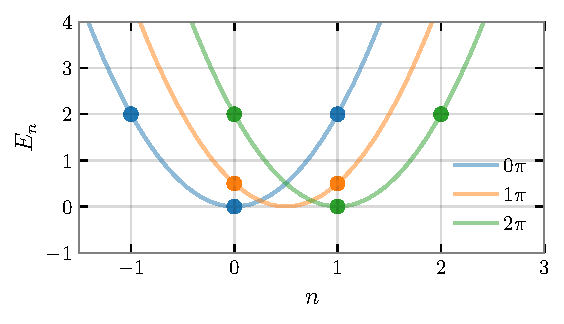
\includegraphics[width=0.6\textwidth]{figs/november/spectrum-particle-on-ring.pdf}
	\caption{}
	\label{fig:particle-on-ring-spectrum}
\end{figure}

Before doing so, we quickly solve this system. The canonical momentum 
corresponding to the above Lagrangian is 
\begin{equation*}
	p \equiv \frac{\partial L}{\partial \dot{x}}
		= m\dot{x} + \frac{\theta}{2\pi}
		\quad \Longrightarrow \quad 
		\dot{x} = \frac{1}{m}\left(p - \frac{\theta}{2\pi}\right)
\end{equation*}
Which means that the Hamiltonian is 
\begin{align*}
	H &= p\dot{x} - L
		= p\cdot \frac{1}{m}\left(p - \frac{\theta}{2\pi}\right)
			- \frac{m}{2}\frac{1}{m^2} \left(p - \frac{\theta}{2\pi}\right)^2 
			- \frac{\theta}{2\pi} \frac{1}{m}\left(p - \frac{\theta}{2\pi}\right)\\
		&= \frac{p^2}{m} - \frac{1}{2m}\left(p^2 - \frac{p\theta}{2\pi} + \frac{\theta^2}{(2\pi)^2}\right)
			+ \frac{\theta^2}{(2\pi)^2 m}\\ 
		&= \frac{p^2}{2m} - \frac{p\theta}{2\pi m} + \frac{\theta^2}{2(2\pi)^2 m}
		= \frac{1}{2m}\left(p - \frac{\theta}{2\pi}\right)^2
\end{align*}
Promoting this to an operator: 
\begin{equation*}
	\hat{H} = \frac{1}{2m}\left(\hat{p} - \frac{\theta}{2\pi}\right)^2
\end{equation*}
So the Schr\"odinger equation is 
\begin{equation*}
	\frac{1}{2m}\left(- i\partial_x - \frac{\theta}{2\pi}\right)^2 \psi_n(x) 
		= E_n\psi_n(x)
\end{equation*}
Since we're trying to be quick, we just Fourier transform: 
\begin{equation*}
	\frac{1}{2m}\left(n - \frac{\theta}{2\pi}\right)^2 
		e^{inx} = E_n e^{inx}
\end{equation*}
which means that the wavefunctions and energies are 
\begin{equation}\label{eq:particle-on-ring-eigenstates}
	\psi_n(x) = \braket{x}{n} = \frac{1}{\sqrt{2\pi}}e^{inx},\qquad 
		E_n = \frac{1}{2m}\left(n- \frac{\theta}{2\pi}\right)^2
\end{equation}

The spectrum is discrete but infinite, as is expected from Pontryagin dual 
of $ \text{U}(1) $ being $ \mathbb{Z} $. The fact that the spectrum is infinite is necessary 
for it to be invariant with respect to $ \theta \rightarrow \theta + 2\pi $ as this 
transformation takes $n \rightarrow n+1 $: 
\begin{equation*}
	E_n = \frac{1}{2m}\left(n + \frac{\theta}{2\pi}\right)^2 
		\rightarrow 
		\frac{1}{2m}\left(n + \frac{\theta + 2\pi}{2\pi}\right)^2 
		= \frac{1}{2m}\left(n + 1 + \frac{\theta}{2\pi}\right)^2 = E_{n+1}
\end{equation*}

From \cref{eq:particle-on-ring-eigenstates} we can read off the action of 
the parity $ P $ and translation (by $ \alpha $) operators $ T_\alpha $: 
\begin{equation*}
	P \ket{n} = \ket{-n},\qquad 
	T_\alpha\ket{n} = e^{in\alpha}\ket{n}
\end{equation*}
where the last line holds because we have $ \psi_n(x) \rightarrow \psi_n(x+ \alpha) $
which is $ e^{in(x+\alpha)} = e^{in\alpha}e^{inx} $. This is just the statement 
that the state $ \ket{n} $ carries translation charge $ n $. 

\begin{figure}[t]
	\centering
	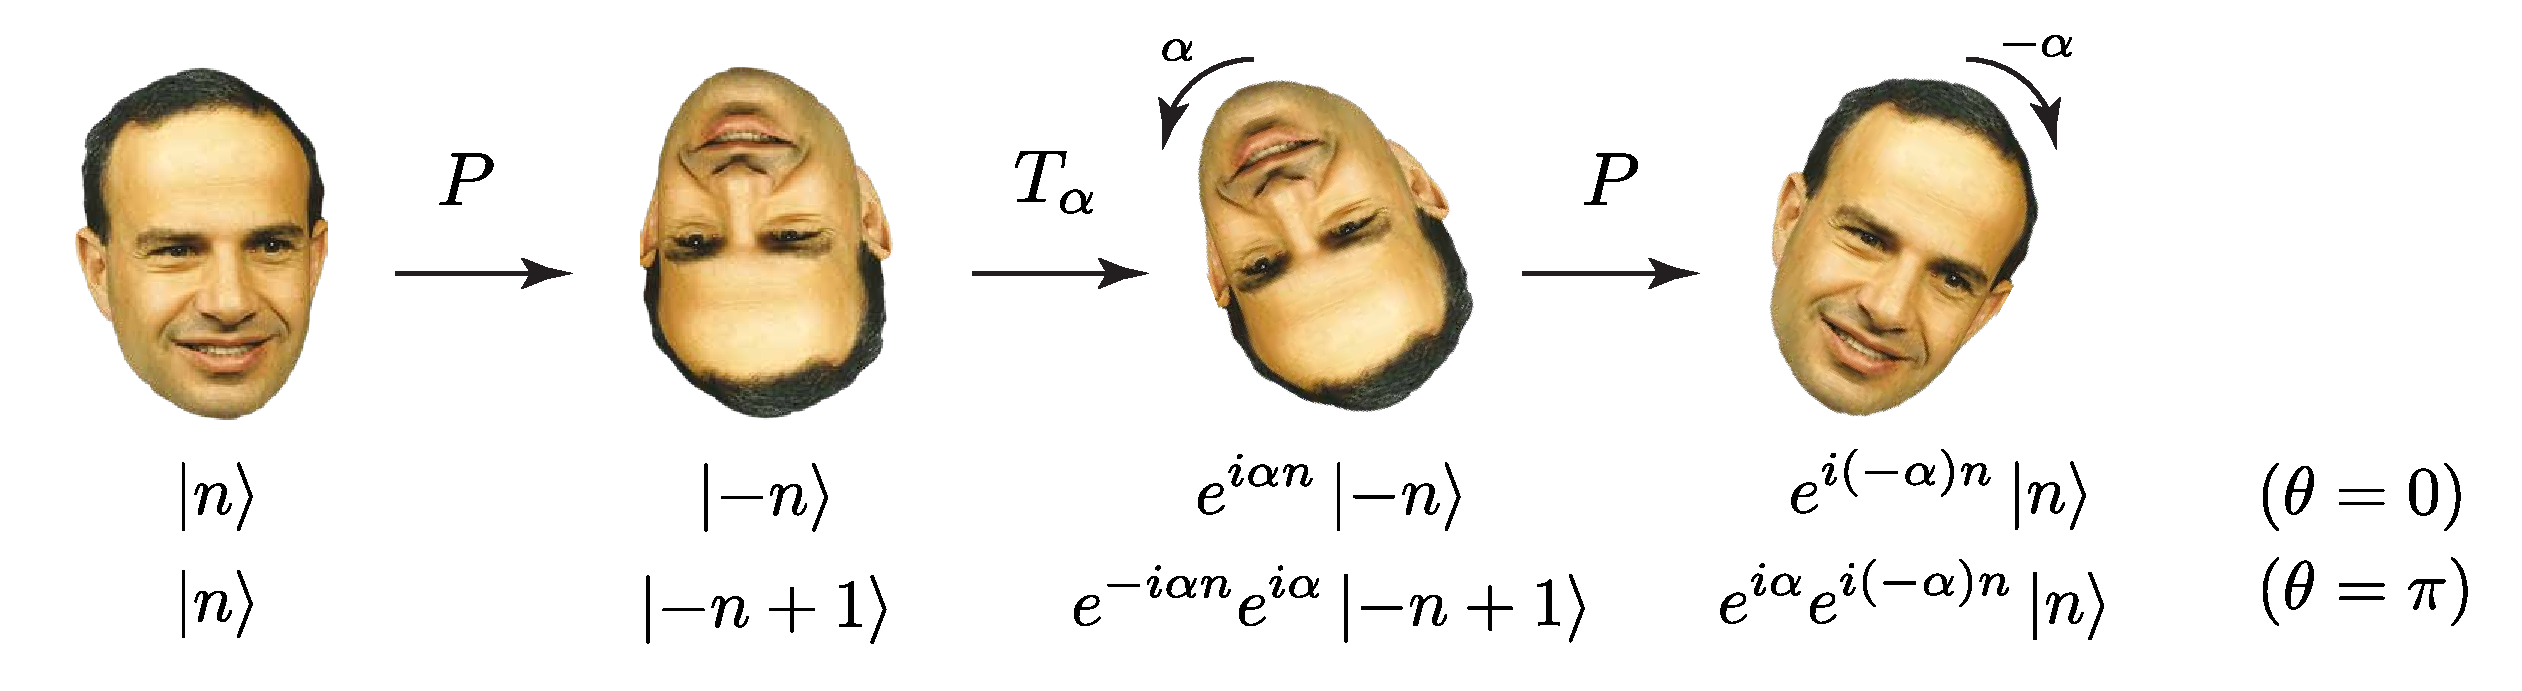
\includegraphics[width=\textwidth]{figs/november/seiberg-thooft-anomaly-vector.pdf}
	\caption{Nati Seiberg demonstrates the action of the parity and translation 
	transformations.}
	\label{fig:particle-on-ring-seiberg}
\end{figure}

\parhead{The anomaly is the central extension}
Now return to the case of $ \theta = \pi \sim -\pi $. This system has a doubly-degenerate 
ground state:
\begin{align*}
	E_n = \frac{1}{2m}\left(n + \frac{1}{2}\right)^2 
	= 
	\frac{1}{2m} \left(-n + 1 + \frac{1}{2}\right)^2
	\Longrightarrow E_0 = E_1 = \frac{1}{2m}\left(\frac{1}{2}\right)^2
\end{align*}
(I think there's a subtlety here---if you decide to show this by leveraging 
$ \theta= \pi\sim -\pi $, you can make the same argument to show that 
$ E_{n} = E_{-n} $ which we will find below that is not the case. Thus I'm pretty 
sure you can't use the fact that $ \pi \sim-\pi $ when discussing the spectrum.)
When $ \theta=0 $ this is not the case: there is a unique ground state $ \ket{n=0} $. 
In fact, generally, we expect that because $ \text{O}(2) $ is a symmetry 
of the Hamiltonian, the eigenstates \cref{eq:particle-on-ring-eigenstates} 
furnish a representation of $ \text{O}(2) $, with each set of degenerate 
eigenstates transforming as an irreducible representation of $ O(2)$. We 
see that when $ \theta = 0 $ this is indeed the case, for $ \ket{n} $ and 
$ \ket{-n} $ share energy $ E_{\pm n} = n^2/2m $: the degenarate states furnish 
the two-dimensional irreps of $ \text{O}(2) $ for they transform into each other
under parity: $ \ket{n} \rightarrow \ket{-n} $. I'm not sure if the ground state 
uniqueness $ \theta=0 $ has a deeper meaning---prima facie, this is a consequence 
of that eigenstate carrying no translation charge. Either way, by this reasoning, 
we have 
\begin{equation*}
	\ket{n} \xrightarrow{P} \ket{-n} \xrightarrow{T_\alpha} e^{-i\alpha n}\ket{-n} 
		\xrightarrow{P} e^{i(-\alpha)n}\ket{n}
\end{equation*}
so that when $ \theta = 0 $, 
\begin{equation*}
	P T_\alpha P = T_{-\alpha}
\end{equation*}
which is demonstrated in \cref{fig:particle-on-ring-seiberg}. 

\begin{alertbox}[Aside]
It's worth emphasizing that this is a very common (I do not know of any
counterexamples) property of degeneracy, which I already discussed a bit 
in \S \ref{sec:symmetries-degeneracy}: eigenstates with the same energy are 
related to each other by symmetry transformations, so the degenerate blocks of 
the Hamiltonian are irreps* of the symmetry group. (*We will see that they can
also be irreps of the central extension instead.)
\end{alertbox}

When $ \theta=\pi $, however, something special happens. We have argued above 
that for this value of $ \theta $ the eigenstates $ \ket{n} $ and $ \ket{-n+1} $
are degenerate: thus, it is those states, not $ \ket{\pm n} $, that transform 
under the irreps of the symmetry of the Hamiltonian. This has the funny 
consequence that 
\begin{equation*}
	\ket{n} 
	\xrightarrow{P} \ket{-n + 1} 
	\xrightarrow{T_\alpha} e^{-i\alpha n} e^{i \alpha}\ket{-n+1}
	\xrightarrow{P} e^{i\alpha} e^{i(-\alpha) n}\ket{n}
	\quad \Longrightarrow  \quad 
	P T_{\alpha} P = e^{i\alpha} T_{-\alpha}
\end{equation*}
which is rooted in the fact that $ \ket{-n + 1} $ has a different translation 
charge than $ \ket{n} $. The states thus no longer transform under a 
faithful representation (TODO check defn faithful) of $ \text{O}(2) $; 
instead, they transform under a projective representation of $ \text{O}(2) $
and thus a representation of the central extension of $ \text{O}(2) $. 

If we gauge the $ U(1) $ symmetry by adding a background gauge field $ A_0 $ to
this theory with $ \dot{x} \rightarrow \dot{x} + A_0 $, and subsequently include
a Chern-Simons term $ kA_0 $, we see the sense in which 't Hooft anomalies 
are thought of as ``obstructions to gauging.'' The action is 
\begin{equation*}
	\int dt \; \frac{m}{2}(\dot{x} + A_0)^2 
		+ \frac{\theta}{2\pi}(\dot{x} + A_0) + k A_0
\end{equation*}
where the $ \text{U}(1) $ is now $ x \rightarrow x + \alpha(t) $ and the 
Lagrangian is gauge invariant if we choose $ A \rightarrow A - \dot{\alpha}(t) $
for the gauge field and, as usual, enforce integer Chern level $ k\in
\mathbb{Z}$. 

In the past we argued that the periodicity in $ \theta $ is a consequence of 
the invariance of the partition function in shifts by $ 2\pi $. This is almost 
the case here, except the action accrues a change in the Chern level: 
\begin{equation*}
	 \frac{\theta+ 2\pi}{2\pi}(\dot{x} + A_0)
		+ kA_0
	= \underbrace{\frac{\theta+ 2\pi}{2\pi}\dot{x}}_{\text{Still invariant}}
		+ \frac{\theta}{2\pi}A_0 + A_0 + k A_0
	= \frac{\theta}{2\pi}(\dot{x} + A_0) + (1+p)A_0
\end{equation*}

Now for the parity symmetry: we postulate this symmetry also takes $ A_0
\rightarrow -A_0$ and
\begin{equation*}
	\frac{m}{2}(\dot{x} + A_0)^2 
		+ \frac{-\theta}{2\pi}(\dot{x} + A_0) - k A_0
\end{equation*}
At $ k=0 $, $ \theta=0 $ this is still a good symmetry of the theory, although 
almost trivially so. At $ \theta=\pi $
\begin{equation*}
	\frac{m}{2}(\dot{x} + A_0)^2 
		+ \frac{-\pi}{2\pi}(\dot{x} + A_0) - k A_0
\end{equation*}
to restore the initial form of the Lagrangian and establish that it is invariant,
we must shift $ \theta \rightarrow \theta +2\pi $ for this induces $ -\pi
\rightarrow -\pi + 2\pi = \pi $. However, we have just argued that this shift 
changes the Chern level to $ -k \rightarrow -k-1 $; there is no $ k $ satisfying 
$ -k -1 = k $ and we conclude that there is no Chern level such that the 
action is invariant under parity. No matter what, a parity transformation 
which induce a change in the Chern level. Notice that this means that even 
if there is \textit{no} Chern-Simons term (Chern level $ k=0 $) the action 
is not invariant; i.e., the obstruction to gauging does not require a Chern-Simons 
term. Something like this comes up in \S \cref{sec:heisenberg-qed3}. This is
what is meant when people speak of a \textit{mixed} 't Hooft anomaly: gauging
translation symmetry breaks parity symmetry. (I have heard, but am not
convinced, that this means that gauging parity would conversely break
translation, and that this is a general feature of mixed anomalies.) 

\parhead{Dynamical consequences} Consider a potential that explicitly breaks 
the $ \text{SO}(2) $ translation symmetry to $ \mathbb{Z}_2 $. One such 
potential is 
\begin{equation*}
	L = \frac{m}{2}\dot{x}^2 + \frac{\theta}{2\pi}\dot{x} 
		+ \lambda \cos 2x
\end{equation*}
which breaks translations $ \left\{T_\alpha\right\} $ to $ \left\{T_0,
T_\pi\right\} $. The symmetry group of $ \theta=0 $ is $ \mathbb{Z}_2 \times 
\mathbb{Z}_2 $, but the symmetry group of $ \theta=\pi $ obeys 
\begin{equation*}
	PT_\pi P = -T_\pi
\end{equation*}
By choosing $ r = P $ and $ t = T_\pi P $ it is not hard to show that this 
makes up the group $ D_4 $, the dihedral group of the square. The
\href{https://proofwiki.org/wiki/Dihedral_Group_D4/Matrix_Representation}{irreducible
representations} of $ D_4 $ are of dimension 2:
\begin{equation*}
	I = \begin{bmatrix}
		1 & 0 \\ 0 & 1 
	\end{bmatrix},\qquad 
	R = - I \quad \text{(reflection)},\qquad
	T = \begin{bmatrix}
		0 & -1 \\ 1 & 0
	\end{bmatrix}\quad  (\pi/2 \text{ rotation}),
\end{equation*}
and all possible products of these matrices. Notably this is \textit{not} 
$ \mathbb{Z}_2\times \mathbb{Z}_2 $.

\subsection{Separating into topological sectors}
To calculate the partition function of this system we can perform a trick 
where we separate the field configurations into different topological sectors; 
i.e., field configurations with different winding numbers. 
This is done by isolating the topological terms and rewriting the path 
integral as a sum over the topological charges $ Q $
\begin{equation*}
	Z = \int \mathcal{D} \phi \;
			e^{i S[\phi] + i S_{\text{top}}[\phi]}
		= \sum_{Q = -\infty}^{\infty} e^{iA Q}
			\int \mathcal{D}\phi_Q \;e^{S[\phi]}	
\end{equation*}
where $ S_{\text{top}}[\phi]$ denotes the topological term, $ A $ 
is some factor associated with it, and $ \mathcal{D}\phi_Q $ denotes field
configurations with the particular winding number $ Q $. 

\begin{figure}[t]
	\centering
	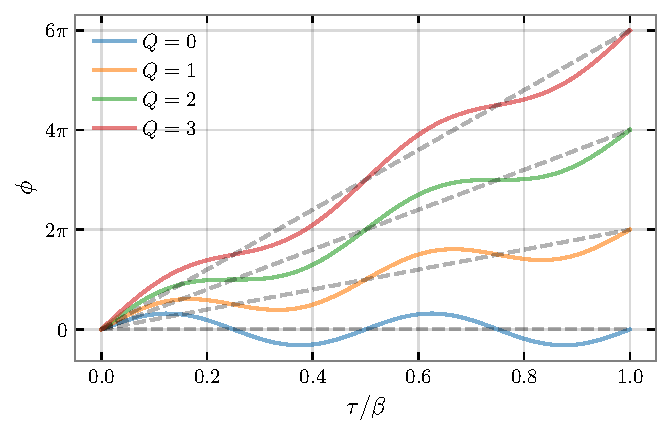
\includegraphics[width=0.6\textwidth]{figs/november/winding-number-particle-on-ring.pdf}
	\caption{Field value $ \phi(\tau) $ for a particle on a ring with various
	winding numbers $ Q $ and for a fixed mode $ \ell = 4 $ (see
	\cref{eq:particle-on-ring-fourier}). The periodicity of general Fourier
	components (i.e., arbitrary $ \ell $) ensures that indeed $
	\phi(\beta) - \phi(0) = 2\pi Q  $.}
	\label{fig:particle-on-ring-winding-number}
\end{figure}

\parhead{Particle on a ring} For a particle on a ring with Wick-rotated path
integral 
\begin{equation}\label{eq:particle-on-ring-partition}
	Z = \int \mathcal{D}\phi \;\exp - \int_0^\beta d\tau 
		\left[
			\frac{m}{2}\dot{\phi}^2 - \frac{i\theta}{2\pi}\dot{\phi}
		\right]
\end{equation}
we can Fourier-expand as 
\begin{equation}\label{eq:particle-on-ring-fourier}
	\phi(\tau) 
		= \frac{2\pi}{\beta}Q \tau + \sum_\ell \phi_\ell
		e^{\frac{2\pi\ell}{\beta}\tau} 
\end{equation}
where again $ Q $ is the topological charge or winding number.That this 
is the winding number can be seen in \cref{fig:particle-on-ring-winding-number}.
Note that $ \phi(\tau) $ is real and thus the reality condition is enforced: 
$ \phi_\ell^\ast = \phi_{-\ell} $.
The derivatives are 
\begin{gather*}
	\dot{\phi} = \frac{2\pi}{\beta}\left(
		Q + \sum_{\ell \in \mathbb{Z}} \phi_\ell e^{\frac{i2\pi\ell\tau}{\beta}}
			\ell i 
			\right)\\
	\dot{\phi}^2 
		= \left(\frac{2\pi}{\beta}\right)^2 
		\left(Q^2 - \sum_{\ell\ell'}\phi_\ell \phi_{\ell'}
			e^{i\frac{2\pi}{\beta}(\ell + \ell') \tau} \ell \ell'
			+ 2 Q \sum_\ell i\ell e^{i\frac{2\pi}{\beta}\phi_\ell}
		\right)
\end{gather*}
and correspondingly \cref{eq:particle-on-ring-partition} reads
\begin{equation*}
	Z = \sum_{Q=-\infty}^{\infty} \int \prod_\ell d\phi_\ell \;
	e^{-S[\phi_\ell, Q]}
\end{equation*}
with 
\begin{align*}
	S &=  - 
	\int_0^\beta d\tau \Bigg[
			\frac{m}{2}\left(\frac{2\pi}{\beta}\right)^2 
				\left(
					Q^2 - {\color{myblue}\sum_{\ell\ell'}
						\phi_\ell \phi_{\ell'}
						e^{\frac{i2\pi}{\beta}(\ell + \ell')\tau }\ell \ell'}
						+ 2Q {\color{myred}\sum_\ell i\ell e^{\frac{i2\pi}{\beta}\ell \tau}
							\phi_\ell }
							\right)\\
					&\qquad\qquad  \qquad
					 - i\frac{\theta}{2\pi} \frac{2\pi}{\beta}
					\left(Q + {\color{myred}\sum_\ell \phi_\ell
					e^{i\frac{2\pi}{\beta}\ell\tau}\ell i}\right)
		\Bigg]
\end{align*}
Now we carry out the $ \beta $ integral, which in this Fourier decomposition 
will induce a number of simplifications by the orthogonality of the modes. 
Namely:
\begin{gather*}
	\int_0^\beta {\color{myblue}\sum_{\ell\ell'}
					\phi_\ell \phi_{\ell'}
					e^{\frac{i2\pi}{\beta}(\ell + \ell')\tau }\ell \ell'}
		= \beta\sum_\ell \phi_\ell \phi_{\ell'} \ell \ell' \delta(\ell+\ell')  
		=- \beta \sum_\ell \ell^2 \phi_\ell \phi_{-\ell} \\
	\int_{0}^{\beta}
		{\color{myred} 
		\sum_\ell \phi_\ell
		e^{i\frac{2\pi}{\beta}\ell\tau}\ell
		}
		=  \int_{0}^{\beta}
		\sum_\ell \phi_\ell \ell
		e^{i\frac{2\pi}{\beta}\ell\tau}
		e^{i\frac{2\pi}{\beta}(0)\tau}
		= \sum_\ell \phi_\ell \ell \delta(\ell - 0)
		= 0
\end{gather*}
We are thus left with 
\begin{align*}
	S &=  \frac{m}{2}\frac{(2\pi)^2}{\beta}
				\left(
					Q^2 - \sum_{\ell}\ell^2 \phi_\ell \phi_{-\ell}
							\right)
					 + i\theta Q
\end{align*}
and the partition function is 
\begin{equation}\label{eq:particle-on-ring-partition-topological}
	Z = \sum_Q 
		e^{-\frac{m}{2} \frac{(2\pi)^2}{\beta}Q^2 + i\theta Q}
		\int \prod_\ell \phi_\ell \exp\left(
			-\frac{m}{2}\frac{(2\pi)^2}{\beta}\sum_\ell \ell^2 
				\phi_\ell \phi_{-\ell}
		\right)
\end{equation}
The $ \phi_\ell $ integral is Gaussian with 
\begin{equation*}
	\int \prod_\ell d\phi_\ell \exp\left(\vec{\phi}^\ast A \vec{\phi}\right),
	\qquad A_{\ell\ell'} = \delta_{\ell\ell'}\ell^2 \frac{m(2\pi)^2}{\beta}
\end{equation*}
which yields the functional determinant 
\begin{equation*}
	\sqrt{\det\left( \frac{\beta \delta_{\ell\ell'}}{2\pi m\ell^2}\right)}
	= \sqrt{\prod_\ell \frac{\beta}{2\pi m\ell^2}} \equiv  \mathcal{N}_\phi
\end{equation*}
(note to self: determinant of diagonal matrix is the product of the diagonals 
not the sum, dummy!) We treat this as an overall constant $ \mathcal{N}_\phi $.
For the topological sector, we use the sum formula (which can be derived 
with the Poisson summation formula)
\begin{equation*}
	\sum_{m = \infty}^{\infty} 
		\exp\left[- \frac{1}{2}Am^2 + iB m\right]
			= \sqrt{\frac{2\pi}{A}}
				\sum_{n = \ell}^{\infty} 
				\exp\left[-\frac{1}{2A} (B - 2\pi n)^2\right]
\end{equation*}
To find that 
\begin{equation*}
	\sum_Q 
		\exp \left(-\frac{m}{2} \frac{(2\pi)^2}{\beta}Q^2 + i\theta Q\right)
		= \sqrt{\frac{\beta}{2\pi m}} \sum_{n=-\infty}^{\infty}
			\exp\left(-\frac{\beta}{2m(2\pi)^2} (\theta - 2\pi n)^2\right)
\end{equation*}
and in aggregate the partition function becomes 
\begin{equation*}
	Z =  \mathcal{N}_\phi \frac{\beta}{2\pi m}\sum_n \exp \left[
		- \frac{\beta}{2m}\left(\frac{\theta}{2\pi} - n\right)^2
	\right]
\end{equation*}
(This $ \beta $ dependence outside the sum is a little funny, but I'm pretty 
sure it's right.)
Since it should have the form $ Z \propto \sum_n \exp(-\beta E_n) $, we can 
immediately read off the spectrum of this system:
\begin{equation*}
	E_n = \frac{1}{2m}\left(\frac{\theta}{2\pi} - n\right)^2.
\end{equation*}

\subsection{Metric Independence of Topological Term}

With that, the action of the particle on a ring is 
\begin{equation}\label{eq:particle-on-ring-tp}
	S = \int dt_p \left(
		\frac{m\dot{\phi}^2}{2} - \frac{\theta}{2\pi} \dot{\phi}
	\right)
\end{equation}
where we have written $ t $ as $ t_p $ to signal that the action takes this form 
for a proper time coordinate $ t_p $. We can parametrize $ t_p = f(t) $ so that  
$ dt_p = f'dt  $, $ dt^2_p = f'^2 dt^2 $ and identify $ f'^2  =g_00 $, 
$ g^00 = f'^{-2} $ as the metric.  

We then find that 
\begin{equation*}
	\frac{d\phi}{dt_p} = \frac{dt}{dt_p} \frac{d\phi}{dt} = \frac{1}{f'}
		\frac{d\phi}{dt}
\end{equation*}
and \cref{eq:particle-on-ring-tp} will become 
\begin{equation*}
	\int dt f' \left[
		\frac{m}{2}\frac{1}{f'^2} \left(\frac{d \phi}{d t}\right)^2
		 - \frac{\theta}{2\pi} \frac{1}{f'} \frac{d \phi}{dt}
	\right]
	=
	\int dt \left[
		\frac{m}{2}\frac{1}{\sqrt{g}} \left(\frac{d \phi}{d t}\right)^2
		 - \frac{\theta}{2\pi} \frac{d \phi}{dt}
	\right]
\end{equation*}
Observe that the $ \theta $ term is then 
\begin{equation*}
	\int dt f'\left(
		- \frac{\theta}{2\pi} \frac{1}{f'} \frac{d \phi}{dt}
	\right)
	= -\int dt \frac{\theta}{2\pi} \frac{d \phi}{dt}
	= - \int \frac{\theta}{2\pi} d\phi
\end{equation*}
which is indeed independent of the metric.

Now, using the considerations of \cref{eq:stress-energy-from-lagrangian}, we 
find that topological term does not contribute to the stress-energy tensor
\begin{equation*}
	\frac{\delta S}{\delta g_{\mu\nu}}
		= - \frac{m}{2} \frac{1}{g} \left(\frac{\delta \sqrt{-g}}{\delta g}\right)
			\frac{d \phi}{dt}
		= - \frac{m}{2}\frac{1}{g}\left(\frac{1}{2}\sqrt{g}g_{\mu\nu}\right)
			\frac{d \phi}{dt}
\end{equation*}
And the stress energy tensor is 
\begin{equation*}
	T_{\mu\nu}
		= - \frac{2}{\sqrt{-g}} \frac{\delta S}{\delta g_{\mu\nu}}
			= \frac{m}{2} \frac{g_{\mu\nu}}{g} \frac{d \phi}{dt}
\end{equation*}
and indeed $ T_{00} $ is the energy: 
\begin{equation*}
	T_{00} = \frac{m}{2} \frac{f'}{f'^2} \frac{d \phi}{dt}
		= \frac{m}{2} \frac{d \phi}{dt}.
\end{equation*}

\subsection{Comments on topological terms}\label{sec:total-derivatives}
\parhead{Total derivatives} Total derivative terms in the Lagrangian do not contribute to the classical 
dynamics (the Euler-Lagrange equations are unchanged). With a total derivative 
term $ \partial_\mu F^\mu = dF $ we can use Stokes theorem:
\begin{equation*}
	S = \int d^d x \; \partial_\mu F^\mu 
		= \int d F  \Longrightarrow S = \int_{\partial_M} F 
\end{equation*}
this is a boundary integral which typically will vanish if we enforce that $ F $
vanishes on the boundary. Of course, at the full quantum level, the manner in
which gauge fields might wind around to the spacetime boundaries will be
detected by the phase of the path integral (see e.g., Coleman, \textit{Aspects
of Symmetry}; for this reason they are sometimes referred to as boundary terms)
even if they vanish at infinity as required, hence these total derivative terms
are topological. 

TODO: understand \href{https://physics.stackexchange.com/questions/262660/two-definitions-of-topological-terms-in-field-theory}{this}.

\parhead{Metric dependence of Hodge star} It is worth noting that the presence 
of certain operations in the term automatically rules out the term as topological. 
For instance, while the wedge product $ \wedge $ makes no reference to a metric 
and thus is allowed, while the Hodge star depends on the metric and thus it
cannot be present in a topological term. This can be seen from its defining 
property: If $ \alpha,\beta \in \bigwedge^k V $ for an $ n $-dimensional vector 
space and $ \omega \in \bigwedge^n V $ is an $ n $-volume form, $ \star\beta $ 
is unique $ (n-k)$-form such that 
\begin{equation*}
	\alpha \wedge (\star \beta) = \langle \alpha,\beta \rangle \omega
\end{equation*}
(in fact, explicitly, it is defined for $ \alpha\in \bigwedge^k V $ as
\begin{equation*}
	\star\alpha 
		= \frac{\color{myred}\sqrt{g}}{(n-k)! k!} 
			\alpha^{i_1,\dots,i_k}\epsilon_{i_1, \dots, i_n}
				dx^{i_{k+1}}\wedge \cdots \wedge dx^{i_n}.
\end{equation*}
which manifestly makes mention of the metric). One way we can understand this 
is that $ \star $ needs knowledge of the metric to scale the $ (n-k) $-form 
$ \star\beta $ properly so that it is related to $ \beta $ in a way that is 
useful and unique.


\subsection*{References}
\begin{itemize}[nosep]
	\item Shao, \textit{Anomalies of Global Symmetries}, [\href{https://youtu.be/2vTvHYYl1Qk?si=ZWlYzvsV2Sp_n43G}{YouTube}].
	\item Seiberg, \textit{Anomalies in the Space of Coupling 
	Constants}, [\href{https://arxiv.org/abs/1905.09315}{arxiv:1905.09315}].
	\item Seiberg, \textit{Theta, Time Reversal, and Temperature} [\href{https://arxiv.org/abs/1703.00501}{arxiv:1703.00501}].
	\item Abanov, \textit{Topology, geometry and quantum interference in condensed matter physics}
	[\href{https://arxiv.org/abs/1708.07192}{arxiv:1708.07192}].
	\item Tong, \textit{Gauge Theory}, \S 3.5.
\end{itemize}

\section{Clifford Algebra Cheat Sheet}
\begin{equation*}
	\text{1+1:} \qquad \gamma^0 = \sigma_z,\quad 
		\gamma^1 = -i\sigma_y, \quad \gamma^5 = \gamma^0\gamma^1
\end{equation*}
{\color{myred} TODO: add also all the identities I've found myself using}

\section{Quantum Integrability, Conserved Quantities}
\begin{itemize}
	\item Integrability vs solvability
	\item Relation to Bethe Ansatz, Yang-Baxter
	\item Relation to presence of conserved quantities. 
\end{itemize}

\section{Stress-Energy from Lagrangian}\label{eq:stress-energy-from-lagrangian}
The stress-energy tensor can be defined as the variation in the action with
respect to the metric (see e.g., Caroll, \textit{Spacetime and Geometry} \S
4.3):
\begin{equation*}
	T_{\mu\nu}
		= - \frac{2}{\sqrt{-g}} \frac{\delta S_\text{M}}{\delta g_{\mu\nu}}
		= - \frac{2}{\sqrt{-g}} 
			\frac{\partial }{\partial g^{\mu\nu}}(\mathcal{L}_{\text{M}} \sqrt{-g})
\end{equation*}
where the subscript $ M $ denotes the action/Lagrangian of the matter fields. 
Had we considered the Einstein-Hilbert action along with the matter fields, 
we would've recovered the Einstein equation.
Calculating this derivative will involve differentiating a determinant ($ g $)
with respect to to a particular entry of the matrix ($ g_{\mu\nu} $). Here is 
how one does this: start with the matrix identity 
\begin{equation*}
	\ln \det M = \tr \ln M 
\end{equation*}
where considering a variation in $ M $ we find this equation becomes 
\begin{align*}
	\delta(\ln \det M) &= \delta(\tr \ln M) \\ 
	\frac{1}{\det M} \delta \det M &= \ln (M^{-1} \delta M)\\ 
	\delta (\det M) &= \det M\cdot \tr (M^{-1} \delta M)
\end{align*}
Identifying $ \det M = \det g_{\mu\nu} = g $ and using the fact that 
$ \delta g_{\mu\nu} = -g_{\mu\rho} g_{\nu\sigma} \delta g^{\rho \sigma}$:
\begin{align*}
	\delta g = g \tr (g^{\lambda \mu} \delta g_{\mu\nu})
			 = g \tr (g^{\lambda\mu} (-1) g_{\mu\rho}g_{\nu\sigma} \delta g^{\rho\sigma})
			 = -g \tr (g_{\nu\sigma} \delta g^{\rho\sigma}) 
\end{align*}
so that taking the trace we find 
\begin{equation*}
	\delta g = - g \;  g_{\mu\nu} \delta g^{\mu\nu}
\end{equation*}
In particular this means that 
\begin{equation*}
	\frac{\partial g}{\partial g_{\mu\nu}} = -g g_{\mu\nu},\qquad 
	\frac{\partial \sqrt{-g}}{\partial g_{\mu\nu}} 
		= - \frac{1}{2} \sqrt{-g} \;g_{\mu\nu}.
\end{equation*}

\chapter{December}
\begin{tocbox}
	\minitoc
\end{tocbox}

\section{Off-Diagonal Matrix Elements for VMC}
In Variational Monte Carlo (VMC) simulations we calculate observables by 
weighting a function $ f(\alpha) $ by a Monte Carlo weight $ \rho(\alpha) $
by a random walk through configurations $ \alpha $ with Metropolis-Hastings 
acceptance criteria: 
\begin{equation*}
	\langle \mathcal{O} \rangle
		= \sum_\alpha f(\alpha)\rho(\alpha),\qquad 
		f(\alpha) = \sum_\beta \bra{\alpha}\mathcal{O}\ket{\beta}
			\frac{\braket{\beta}{\psi}}{\braket{\alpha}{\psi}},\quad 
			\rho(\alpha) = \frac{|\braket{\alpha}{\psi}|^2}{\braket{\psi}}
\end{equation*}
$ \rho(\alpha) $ is accounted for by the acceptance probability 
\begin{equation*}
	P(\alpha \rightarrow \alpha') 
		= \begin{cases}
		1 & \rho(\alpha') > \rho(\alpha)\\ 
		\rho(\alpha')/\rho(\alpha) & \rho(\alpha') < \rho(\alpha)
		\end{cases}
\end{equation*}
while $ f(\alpha) $ must be computed at a chosen sample frequency. The best 
case scenario is that $ \mathcal{O} $ is diagonal in the chosen basis 
states $ \alpha $, $ \beta $ over which we are perfoming our random walk. 
Then we just have to calculate 
\begin{equation*}
	f(\alpha) = \bra{\alpha}\mathcal{O}\ket{\alpha}
\end{equation*}
However, oftentimes we will have to compute more complicated expectation 
values which will involve off-diagonal elements. In what follows we work out 
some examples by considering all possible off diagonal elements of spin-1/2 
operators.

Consider $ S^x = (S^+ + S^-)/2$. This operator's only nonvanishing matrix elements 
are 
\begin{equation*}
	\bra{\uparrow} S_x \ket{\downarrow} = 
	\bra{\downarrow} S_x \ket{\uparrow} = \frac{1}{2}
\end{equation*}
This is of course related to the fact that $ S^+ + S^- $ acts by flipping the spin, e.g.,
\begin{equation*}
	(S^+ + S^-)\ket{\uparrow} = \cancel{S^+\ket{\uparrow}}
		+ S^- \ket{\uparrow} = \ket{\downarrow} 
\end{equation*}
For $ S^y = - i (S^+ - S^-) / 2 $, the nonvanishing elements are
\begin{equation*}
	\bra{\uparrow} S_y \ket{\downarrow} = \frac{i}{2},\qquad
	\bra{\downarrow} S_y \ket{\uparrow} = -\frac{i}{2}
\end{equation*}
Now consider these operators as they act on a tensor product Hilbert space.
Let's say $ S_i^x $ acts on a site $ i $:
\begin{equation*}
	\bra{\alpha} S_i^x \ket{\beta}
		= \frac{1}{2}\bra{\alpha} (S^+_i + S^-_i) \ket{\beta}
\end{equation*}
We specialize to half-filling in a Mott insulator phase (no double-occupancy). 
Then there is either a spin up or spin down at the site $ i $. Because 
the operator is understood to flip whatever spin is at that site, and because 
the tensor-product factorization guarantees us that the remaining sites 
in $ \ket{\alpha} $ and $ \ket{\beta} $ must have the same configuration for the
matrix element to be nonvanishing, we conclude that the only nonvanishing matrix
elements $ \bra{\alpha} S_i^x\ket{\beta} $ are those $ \ket{\beta} $ related to 
$ \ket{\alpha} $ only by the flip of the spin at site $ i $. Note that this 
means there is only one such matrix element, and it is off-diagonal.

Now we apply the above reasoning to products of operators. We write 
\begin{equation*}
	\ket{\alpha} = \ket{\sigma_{\alpha 1}}\otimes \cdots \otimes 
			\ket{\sigma_{\alpha N}}
\end{equation*}
(and similarly for $ \ket{\beta} $), and we introduce the ``complement''
\begin{equation*}
\ket*{\alpha_{ij,\dots}^\complement} \equiv \ket{\alpha}\text{ excluding the 
   states on sites }ij\dots
\end{equation*}

% \subsection{Quadratic operators}
\parhead{Quadratic operators} We then find, assuming $ i\neq j $
\begin{align*}
	\bra{\alpha} S_i^x S_j^x \ket{\beta}
	&= \bra*{\alpha_{ij}^\complement} \otimes \bra{\sigma_{\alpha i}}
	\otimes \bra{\sigma_{\alpha j}}
	S_i^x S_j^x \ket{\sigma_{\beta i}} \otimes \ket{\sigma_{\beta j}}
	\otimes \ket*{\beta_{ij}^\complement}\\
	&= \braket*{\alpha_{ij}^\complement}{\beta_{ij}^\complement}
	\bra{\sigma_{\alpha i}}S_i^x \ket{\sigma_{\beta i}}
	\bra{\sigma_{\alpha j}}S_j^x \ket{\sigma_{\beta j}}
\end{align*}
Orthonormality ensures that the factor $ \braket*{\alpha_{ij}^\complement}{\beta_{ij}^\complement} $
vanishes unless the configuration is the same on all sites but $ i$, $ j $. 
We use the notation $ \delta_{\alpha^\complement_{ij} \beta^\complement_{ij}} $ to denote this fact. 
Then we have
\begin{gather*}
	\bra{\alpha} S_i^x S_j^x \ket{\beta}
		= \delta_{\alpha\beta}
			\bra{\sigma_{\alpha i}}S_i^x \ket{\sigma_{\beta i}}
			\bra{\sigma_{\alpha j}}S_j^x \ket{\sigma_{\beta j}}\\
	\bra{\alpha} S_i^y S_j^y \ket{\beta}
		= \delta_{\alpha\beta}
			\bra{\sigma_{\alpha i}}S_i^y \ket{\sigma_{\beta i}}
			\bra{\sigma_{\alpha j}}S_j^y \ket{\sigma_{\beta j}}
\end{gather*}
If $ i = j $ we cannot factor the Hilbert space as we did above, but the 
answer is trivial as $ (S_i^{(x,y)})^2 = 1/4 $. This is rooted in the fact
that the site will always be maximally correlated with itself.

% \subsection{Biquadratic operators}
% The biquadratic term is calculated as follows. Consider 
% \begin{equation*}
% 	\bra{\alpha} S_{k}^x S_{i}^x S_{k}^z S_{j}^z \ket{\beta}.
% \end{equation*}
% If $ i=j= k $, we have 
% \begin{equation*}
% 	\bra{\alpha} (S_k^x)^2 (S_k^z)^2 \ket{\beta}
% 		= \frac{1}{4^2} \delta_{\alpha \beta}.
% \end{equation*}
% (where here and in what follows we assume rotational invariance.)
% If $ k=i\neq j $ or $ k=j\neq i $, 
% \begin{gather*}
% 	\bra{\alpha} S_{k}^x S_{k}^x S_{k}^z S_{j}^z \ket{\beta}
% 		=  \frac{1}{4}\bra{\alpha} S_{k}^z  S_{j}^z \ket{\beta} \\
% 	\bra{\alpha} S_{k}^x S_{i}^x S_{k}^z S_{k}^z \ket{\beta}
% 		=  \frac{1}{4}\bra{\alpha} S_{k}^x  S_{i}^x \ket{\beta} 
% 		=  \frac{1}{4}\bra{\alpha} S_{k}^z  S_{i}^z \ket{\beta} 
% \end{gather*}

% If all three sites $ i, j, k $ are different:
% \begin{align*}
% 	\bra{\alpha} S_{k}^x S_{i}^x S_{k}^z S_{j}^z \ket{\beta}
% 		&= \braket*{\alpha_{ijk}^\complement}{\beta_{ijk}^\complement}
% 			\bra{\sigma_{\alpha k}} S_k^x S_k^z \ket{\sigma_{\beta k}}
% 			\bra{\sigma_{i\alpha}} S_i^x \ket{\sigma_{i\beta}}
% 			\underline{\bra{\sigma_{j\alpha}} S_j^z \ket{\sigma_{j\beta}}}
% \end{align*}
% The last factor (underlined) is diagonal in our chosen basis, so it picks up 
% the eigenvalue of the configurations' spins at that site if they are the same, 
% and zero otherwise: $\sigma_{j\alpha}\delta_{\sigma_{j\alpha}\sigma_{j\beta}}/2$. 
% Then this becomes
% \begin{align*}
% 		&= \delta_{\alpha^\complement_{ijk}\beta^\complement_{ijk}} \frac{\sigma_{j\alpha}}{2}
% 			\delta_{\sigma_{j\alpha}\sigma_{j\beta}}
% 			\bra{\sigma_{\alpha k}} S_k^x S_k^z \ket{\sigma_{\beta k}}
% 			\bra{\sigma_{\alpha i}}S_i^x \ket{\sigma_{\beta i}}
% \end{align*}
% Again since in our chosen basis $ \ket{\sigma_{\beta k}} $ is an eigenstate of 
% $ S_j^z $ with eigenvalue $ \sigma_{\beta k}/2 $, which yields:
% \begin{align*}
% 		&= \frac{1}{4}
% 		\delta_{\alpha^\complement_{ijk}\beta^\complement_{ijk}}	
% 		\delta_{\sigma_{j\alpha} \sigma_{j\beta}}
% 			\sigma_{j\alpha}\sigma_{\beta k} 
% 			\bra{\sigma_{\alpha k}}S_k^x \ket{\sigma_{\beta k}}
% 			\bra{\sigma_{\alpha i}} S_i^x \ket{\sigma_{\beta i}}
% \end{align*}
% Lastly, if $ i=j\neq k $: 
% \begin{align*}
% 	\bra{\alpha} S_k^x S_i^x S_k^z S_i^z\ket{\beta} 	
% 		&= \delta_{\alpha\beta} \bra{\sigma_{\alpha k}}S_k^x S_k^z 
% 			\ket{\sigma_{\beta k}}
% 			\bra{\sigma_{\alpha i}}S_i^x S_i^z\ket{\beta i}\\
% 		&= \frac{1}{4} \delta_{\alpha \beta} \sigma_{\beta k} \sigma_{\beta i}
% 			\bra{\sigma_{\alpha k}} S_k^x \ket{\sigma_{\beta k}}
% 			\bra{\sigma_{\alpha i}} S_i^x \ket{\sigma_{\beta i}}
% \end{align*}
% But note that in our result for $ i\neq j \neq k $, we have $ \sigma_{\alpha j} = 
% \sigma_{\beta j}$, and here we have $ i=j $, so actually our results for 
% $ i\neq j\neq k $ agree with $ i = j \neq k $. 
	
% Futher, note that rotational invariance guarantees that 
% \begin{equation*}
% 	\bra{\alpha} S_k^x S_i^x S_k^z S_j^z\ket{\beta} 	
% 		= \bra{\alpha} S_k^y S_i^y S_k^z S_j^z\ket{\beta}.
% \end{equation*}
% Also note that because the expectation values are real, we have 
% \begin{equation*}
% 	\langle S_k^x S_i^x S_k^z S_j^z\rangle
% 	= \langle S_k^z S_j^z S_k^x S_i^x \rangle
% \end{equation*}
% Note the indices $ i $, $ j $ are swapped (actually, numerical results suggest that
% this holds even if we switch $ i \rightarrow j$). 

% % If we were to switch $ x \leftrightarrow z $ we'd get 
% % \begin{align*}
% % 	\bra{\alpha} S_{k}^z S_{i}^z S_{k}^x S_{j}^x \ket{\beta}
% % 		= \delta_{\alpha\beta} \frac{\sigma_{j\alpha}}{2}
% % 			\delta_{\sigma_{j\alpha}\sigma_{j\beta}}
% % 			\bra{\sigma_{\alpha k}} S_k^z S_k^x \ket{\sigma_{\beta k}}
% % 			\bra{\sigma_{\alpha i}}S_i^x \ket{\sigma_{\beta i}}
% % \end{align*}
% % which means that the eigenvalue we get is that of the configuration $ \alpha $, 
% % not the configuration $ \beta $:
% % \begin{gather*}
% % 	\bra{\alpha} S_{k}^z S_{i}^z S_{k}^x S_{j}^x \ket{\beta}
% % 		= \frac{1}{4}\delta_{\alpha\beta}\delta_{\sigma_{j\alpha} \sigma_{j\beta}}
% % 			\sigma_{j\alpha}\sigma_{\alpha k} 
% % 			\bra{\sigma_{\alpha k}}S_k^x \ket{\sigma_{\beta k}}
% % 			\bra{\sigma_{\alpha i}} S_i^x \ket{\sigma_{\beta i}}\\
% % 	\bra{\alpha} S_{k}^z S_{i}^z S_{k}^y S_{j}^y \ket{\beta}
% % 		= \frac{1}{4}\delta_{\alpha\beta}\delta_{\sigma_{j\alpha} \sigma_{j\beta}}
% % 			\sigma_{j\alpha}\sigma_{\alpha k} 
% % 			\bra{\sigma_{\alpha k}}S_k^y \ket{\sigma_{\beta k}}
% % 			\bra{\sigma_{\alpha i}} S_i^y \ket{\sigma_{\beta i}}
% % \end{gather*}

% With $ S^x = (1/2) (S^+ + S^-) $ and $ S^y = -(i/2) (S^+ - S^-) $ we have 
% \begin{gather*}
% (S^x)^2 = \left(\frac{1}{2}\right)^2 (S^+ + S^-)^2 
% 	= \frac{1}{4}\left(\cancel{(S^+)^2} + S^+ S^- + S^- S^+ + \cancel{(S^-)^2}\right)\\
% (S^y)^2 = \left(-\frac{i}{2}\right)^2 (S^+ - S^-)^2 
% 	= -\frac{1}{4}\left(\cancel{(S^+)^2} - S^+ S^- - S^- S^+ + \cancel{(S^-)^2}\right)
% \end{gather*}
% where the vanishing $ (S^{\pm})^2 $ can be seen from the explicit matrix 
% product or from the fact that you cannot raise the spin twice. Now 
% it turns out that $ S^+ S^- = \ketbra{\uparrow}$ and $ S^- S^+ = \ketbra{\downarrow} $, 
% so 
% \begin{equation*}
% 	(S^x)^2 = \frac{1}{4}, \qquad (S^y)^2 = \frac{1}{4},\qquad 
% 	(S^z)^2 = \frac{1}{4}.
% \end{equation*}
% Then we have 
% \begin{align*}
% 	\bra{\alpha} S_k^x S_i^x S_k^x S_j^x \ket{\beta}
% 		&= \bra{\alpha} (S_k^x)^2 S_i^x S_j^x \ket{\beta}
% 		= \frac{1}{4} \bra{\alpha} S_i^x S_j^x \ket{\beta}\\
% 	&\qquad \Longrightarrow 
% 	\langle S_k^x S_i^x S_k^x S_j^x \rangle 
% 	= \frac{1}{4} \langle S_i^x S_j^x \rangle
% \end{align*}
% The same argument holds for $ S^y $ and $ S^z $, so 
% \begin{equation*}
% 	\langle S_k^x S_i^x S_k^x S_j^x \rangle 
% 	= \frac{1}{4} \langle S_i^x S_j^x \rangle,\qquad
% 	\langle S_k^y S_i^y S_k^y S_j^y \rangle 
% 	= \frac{1}{4} \langle S_i^y S_j^y \rangle,\qquad
% 	\langle S_k^z S_i^z S_k^z S_j^z \rangle 
% 	= \frac{1}{4} \langle S_i^z S_j^z \rangle.
% \end{equation*}

% Lastly we compute the off-diagonal elements for $ S_k^x S_i^x S_k^y S_j^y $. 
% If $ i\neq j\neq k $:
% \begin{align*}
% 	\bra{\alpha} S_k^x S_i^x S_k^y S_j^y \ket{\beta}
% 		= 
% 		\delta_{\alpha^\complement_{ijk}\beta^\complement_{ijk}}	
% 			\bra{\sigma_{\alpha k}} S_k^x S_k^y \ket{\sigma_{\beta k}}
% 			\bra{\sigma_{\alpha i}} S_i^x \ket{\sigma_{\beta i}}
% 			\bra{\sigma_{\alpha j}} S_j^y \ket{\sigma_{\beta j}}
% \end{align*}
% Now note that $ S^x S^y = i S^z /2 $. Then 
% \begin{align*}
% 	\bra{\alpha} S_k^x S_i^x S_k^y S_j^y \ket{\beta}
% 		= \frac{i}{4}
% 		\delta_{\alpha^\complement_{ijk}\beta^\complement_{ijk}}		
% 		\delta_{\sigma_{\alpha k} \sigma_{\beta k}}
% 			\sigma_{\alpha k} \bra{\sigma_{\alpha i}} S_i^x \ket{\sigma_{\beta i}}
% 				\bra{\sigma_{\alpha j}} S_j^y \ket{\sigma_{\beta j}}
% \end{align*}
% Since $ S^y S^x = -iS^z /2 $, we likewise have
% \begin{align*}
% 	\bra{\alpha} S_k^y S_i^y S_k^x S_j^x \ket{\beta}
% 		= - \frac{i}{4} 
% 		\delta_{\alpha^\complement_{ijk}\beta^\complement_{ijk}}		
% 		\delta_{\sigma_{\alpha k} \sigma_{\beta k}}
% 			\sigma_{\alpha k} \bra{\sigma_{\alpha i}} S_i^y \ket{\sigma_{\beta i}}
% 				\bra{\sigma_{\alpha j}} S_j^x \ket{\sigma_{\beta j}}
% \end{align*}
% But note that as in the above, the reality of the expectation value lets us 
% take the adjoint to find
% \begin{equation*}
% 	\langle S_k^x S_i^x S_k^y S_j^y \rangle 
% 		= \langle S_k^y S_j^y S_k^x S_i^x \rangle .
% \end{equation*}

% Following the same reasoning as above, we find that if $ i=j=k $: 
% \begin{equation*}
% 	\bra{\alpha} (S_k^x)^2 (S_k^y)^2 \ket{\beta}
% 		= \frac{1}{4^2} \delta_{\alpha \beta}.
% \end{equation*}
% and if $ k=i\neq j $ and $ k= j\neq i $ respectively: 
% \begin{gather*}
% \bra{\alpha} S_k^x S_k^x S_k^y S_j^y \ket{\beta} 
% 	= \frac{1}{4}\bra{\alpha} S_k^z S_j^z \ket{\beta}\\ 
% \bra{\alpha} S_k^x S_k^j S_k^y S_j^y \ket{\beta} 
% 	= \frac{1}{4}\bra{\alpha} S_k^z S_j^z \ket{\beta}
% \end{gather*}


% To summarize, we have found, assuming rotational invariance, the $ 3^2 = 9 $
% (for each pair of directions) biquadratic terms to be 
% \begin{itemize}
% \item $	\langle S_k^x S_i^x S_k^z S_j^z\rangle = \langle S_k^z S_j^z S_k^x S_i^x \rangle 
% 	= \langle S_k^y S_i^y S_k^z S_j^z\rangle = \langle S_k^z S_j^z S_k^y S_i^y\rangle $ 
% 	with 
% 	\begin{equation*}
% 	\bra{\alpha} S_k^x S_i^x S_k^z S_i^z\ket{\beta} 	
% 		= \begin{cases}
% 			\frac{1}{16} \delta_{\alpha \beta} & i = j =k\\ 
% 			\frac{1}{4}\bra{\alpha} S_{k}^z  S_{j}^z \ket{\beta} & k = i \neq j\\
% 			\frac{1}{4}\bra{\alpha} S_{k}^z  S_{i}^z \ket{\beta} & k = j \neq i\\
% 			\frac{1}{4}
% 			\delta_{\alpha^\complement_{ijk}\beta^\complement_{ijk}}		
% 			\sigma_{\beta k} \sigma_{\beta i}
% 			\bra{\sigma_{\alpha k}} S_k^x \ket{\sigma_{\beta k}}
% 			\bra{\sigma_{\alpha i}} S_i^x \ket{\sigma_{\beta i}} &\text{ otherwise}
% 		\end{cases}
% 	\end{equation*}
% \item $ \langle S_k^x S_i^x S_k^y S_j^y\rangle = \langle S_k^y S_j^y S_k^x S_i^x\rangle$
% with 
% \begin{equation*}
% 	\bra{\alpha} S_k^x S_i^x S_k^y S_j^y \ket{\beta}
% 	= 
% 	\begin{cases}
% 		\frac{1}{16} \delta_{\alpha \beta} & i = j = k\\
% 		\frac{1}{4}\bra{\alpha} S_k^z S_j^z \ket{\beta} & k=j\neq i\\
% 		\frac{1}{4}\bra{\alpha} S_k^z S_j^z \ket{\beta} & k=i\neq j\\
% 		\frac{i}{4}
% 		\delta_{\alpha^\complement_{ijk}\beta^\complement_{ijk}}		
% 		\delta_{\sigma_{\alpha k} \sigma_{\beta k}}
% 		\sigma_{\alpha k} \bra{\sigma_{\alpha i}} S_i^x \ket{\sigma_{\beta i}}
% 		\bra{\sigma_{\alpha j}} S_j^y \ket{\sigma_{\beta j}} & \text{otherwise}
% 	\end{cases}
% \end{equation*}
% \item $\langle S_k^x S_i^x S_k^x S_j^x \rangle 
% 	= \langle S_k^y S_i^y S_k^y S_j^y \rangle 
% 	= \langle S_k^z S_i^z S_k^z S_j^z \rangle 
% 	= \frac{1}{4} \langle S_i^z S_j^z \rangle$.
% \end{itemize}
% Remarkably, this means we only have to compute three different types of 
% observables.

At half-filling ($ N_\uparrow = N_\downarrow $), an additional 
simplification occurs: We are restricted to the sector of Hilbert space with 
fixed number of up and down electrons. Thus, in this sector, any operator
flipping to a different number up or down spins individually will have vanishing 
matrix elements. For instance, $ S_i^x $ flips a single spin and takes 
$ N_\uparrow \rightarrow N_\uparrow - 1 $ and $ N_\downarrow \rightarrow
N_\downarrow + 1 $ or $ N_\uparrow \rightarrow N_\uparrow + 1 $ and $
N_\downarrow \rightarrow N_\downarrow - 1 $. It therefore has vanishing elements 
in this sector. On the other hand, $ S_i^x S_j^x $ has nonvanishing elements 
when it flips spin $ i $ from up to down and spin $ j $ from down to up and 
vice-versa. Note this also means that this operator must act on sites with 
opposite spins. Also note that because the operator will always flip two opposite 
spins, products of operators that depend on the original spin being flipped 
(namely, $ S_i^y S_j^y $) will no longer depend on the original spins. 
This means that we're guaranteed $ \langle S_i^y S_j^y \rangle = 
\langle S_i^x S_j^x \rangle$ since $ (1/2)^2 = -(i/2)^2 $, as should be expected 
from the symmetry of the problem. 

\parhead{Biquadratic operators}
In order to perform a Hamiltonian reconstruction using the correlation matrix, 
one needs knowledge of the biquadratic four-point correlations of the theory 
in addition to the two-point correlators worked out above; i.e., we need 
\begin{equation*}
	\langle S_i^\alpha S_j^\alpha S_k^\beta S_\ell^\beta \rangle,\qquad 
		\alpha,\beta \in \left\{x,y,z\right\}
\end{equation*}
While at first glance the above constitutes $ 3^2 = 9 $ different operators 
corresponding to all possible pairs of directions, a large number of correlators 
are equal to each other provided the wavefunction is rotationally invariant. 
Namely, we have that 
\begin{equation*}
	\langle S_i^x S_j^x S_k^x S_\ell^x \rangle = 
	\langle S_i^y S_j^y S_k^y S_\ell^y \rangle = 
	\langle S_i^z S_j^z S_k^z S_\ell^z \rangle
\end{equation*}
and 
\begin{align*}
	&\langle S_i^x S_j^x S_k^z S_\ell^z \rangle = 
	\langle S_i^y S_j^y S_k^z S_\ell^z \rangle = 
	\langle S_i^x S_j^x S_k^y S_\ell^y \rangle\\
	&\qquad =\langle S_i^z S_j^z S_k^y S_\ell^y \rangle = 
	\langle S_i^y S_j^y S_k^x S_\ell^x \rangle = 
	\langle S_i^z S_j^z S_k^x S_\ell^x \rangle.
\end{align*}
This can be seen by considering the unitary operators $ U[\mathcal{R}] $
that implement the elements of the internal $ \text{SU}(2) $ symmetry in
this representation. 
Consider $ \bra{\psi} S_i^x S_i^x S_j^y S_k^y \ket{\psi} $.
Assuming the Gutzwiller wavefunction transforms trivially under any 
$ U[\mathcal{R}] $ such that $ U[\mathcal{R}]\ket{\psi} = \psi $ (up to a phase), 
we need only identify the group element $ \mathcal{R}' $ taking
\begin{equation*}
	U[\mathcal{R}'] S_i^y U[\mathcal{R}']^{-1}
		= S_i^z
\end{equation*}
and leaving $ S_i^x $ invariant, 
so that inserting $ U[\mathcal{R}']^{-1}  U[\mathcal{R}']$ between every pair 
of operators we find
\begin{align*}
	\bra{\psi} S_i^x S_i^x S_j^y S_k^y \ket{\psi}
		&= 
	\bra{\psi}U[\mathcal{R}']^{-1} S_i^x S_j^x S_k^y S_\ell^y U[\mathcal{R}']\ket{\psi}\\
		&=\bra{\psi} S_i^x S_j^x S_k^z S_\ell^z \ket{\psi}.
\end{align*}
Similar arguments lead to the conclusion that provided the wavefunction transforms 
trivially under the entire symmetry group, the expectation value is invariant 
across the orbit of $ S_i^x S_j^x S_k^y S_\ell^y $ under $ \text{SU}(2) $.
This can be understood as a consequence of the geometric fact that any plane
crossing the origin in $ \mathbb{R}^3 $ can be taken to any other plane.

Thus, in actuality we only need to compute two 
different four-point correlators. The former possess the matrix elements 
\begin{equation*}
	\bra{\alpha} S_i^z S_j^z S_k^z S_\ell^z \ket{\beta} 
		= \frac{1}{16}\delta_{\alpha\beta}\sigma_i\sigma_j\sigma_k \sigma_\ell
\end{equation*}
for we chose a basis diagonal in $ S^z $. The latter operators 
\begin{equation*}
	\langle S_i^x S_j^x S_k^z S_\ell^z \rangle 
\end{equation*}
have a more complicated matrix structure which depends on which operators act at
different sites. Consider $ i=j=k=l $. Then 
\begin{equation*}
	\bra{\alpha} S_i^x S_i^x S_i^z S_i^z \ket{\beta} = 
	\bra{\alpha} (S_i^x)^2 (S_i^z)^2 \ket{\beta} = \frac{1}{16}\delta_{\alpha\beta}
\end{equation*}
Now consider $ i=j $ independent of the other sites. Then we have 
\begin{equation*}
	\bra{\alpha} (S_i^x)^2 S_k^z S_\ell^z \ket{\beta}
		= \frac{1}{4} \bra{\alpha} S_k^z S_\ell^z \ket{\beta}
\end{equation*}
of if $ k=\ell $
\begin{equation*}
	\bra{\alpha} S_i^x S_j^x (S_k^z S_k^z)^2 \ket{\beta}
		= \frac{1}{4} \bra{\alpha} S_i^x S_j^x\ket{\beta}
		= \frac{1}{4} \bra{\alpha} S_i^z S_j^z\ket{\beta}
\end{equation*}
where we've used rotational invariance in the last equality. Thus if any pair 
of $ x $ or $ z $ operators act on the same site we just have to calculate
the two point $ S^z $ correlator for the remaining two sites. 

The case $ i=k \neq j = \ell$ has 
\begin{align*}
	\bra{\alpha} S_i^x S_j^x S_i^z S_j^z \ket{\beta}
		&= \delta_{\alpha^\complement_{ij}\beta_{ij}^\complement}
			\bra{\sigma_{\alpha i}} S_i^x S_i^z\ket{\sigma_{\beta i}}
			\bra{\sigma_{\alpha j}} S_j^x S_j^z\ket{\sigma_{\beta j}}\\
		&= \frac{1}{4} 
			\delta_{\alpha^\complement_{ij}\beta_{ij}^\complement}
			\sigma_{\beta i}\sigma_{\beta j}\bra{\sigma_{\alpha i}} S_i^x \ket{\sigma_{\beta i}}
			\bra{\sigma_{\alpha j}} S_j^x \ket{\sigma_{\beta j}}
\end{align*}
(it is not hard to see that there is only one allowed $ \ket{\beta} $ configuration, 
the one obtained by flipping the spins on sites $ i $ and $ j $. This means 
$ \sigma_{\beta i}= - \sigma_{\alpha i} $). 
If $ j=\ell \neq i \neq k $, we have 
\begin{equation*}
	\bra{\alpha} S_i^x S_j^x S_k^z S_j^z \ket{\beta}
		=\frac{1}{4} \delta_{\alpha_{ij}^\complement \beta_{ij}^\complement}
			\sigma_k \sigma_{\beta j}
			\bra{\sigma_{\alpha i}} S_i^x \ket{\sigma_{\beta i}}
			\bra{\sigma_{\alpha j}} S_j^x \ket{\sigma_{\beta j}}
\end{equation*}
If $ i=k\neq j\neq \ell $ an analogous expression is obtained by swapping $ i\leftrightarrow j $
and $ k\leftrightarrow \ell $: 
\begin{equation*}
	\bra{\alpha} S_i^x S_j^x S_k^z S_\ell^z \ket{\beta}
		= \frac{1}{4}
			\delta_{\alpha_{ij}^\complement \beta_{ij}^\complement}
			\sigma_{\ell} \sigma_{\beta i} 
			\bra{\sigma_{\alpha i}} S_i^x \ket{\sigma_{\beta i}}
			\bra{\sigma_{\alpha j}} S_j^x \ket{\sigma_{\beta j}}.
\end{equation*}

Lastly, if $ i\neq j\neq k\neq \ell $: 
\begin{equation*}
	\bra{\alpha} S_i^x S_j^x S_k^z S_\ell^z \ket{\beta}
		= \frac{1}{4}
			\delta_{\alpha_{ij}^\complement \beta_{ij}^\complement} 
			\sigma_{k}\sigma_{\ell} 
			\bra{\sigma_{\alpha i}} S_i^x \ket{\sigma_{\beta i}}
			\bra{\sigma_{\alpha j}} S_j^x \ket{\sigma_{\beta j}}..
\end{equation*}

\subsection*{References} 
\begin{itemize}[nosep]
\item Gros, \textit{Physics of Projected Wavefunctions} (1988) [\href{https://ui.adsabs.harvard.edu/link_gateway/1989AnPhy.189...53G/doi:10.1016/0003-4916(89)90077-8}{doi:10.1016/0003-4916(89)90077-8}]. 
\end{itemize}

\section{2d CFT Basics}
\epigraph{That book should be banned from classrooms.}{\textit{Antal Jevicki on 
Di Francesco}}

Once upon a time I tried learning some CFT from Di Francesco as a final project
for my intro QFT class. Unsurprisingly for those familiar with that book, 
that did not go well. More recently I picked up Blumenhagen and Plauschinn's 
CFT book and found that it presented the material in a nicely condensed fashion 
(although I still think the bulk of it would've gone over my head as I was 
not sufficiently comfortable with field theory generally back then).

\parhead{The conformal group}
We all know that the derivative $ -i \partial_x $ is the generator of $ x $ translations; 
we can see directly that this is the case by considering the exponential map 
$ \exp(i \epsilon (-i\partial_x) ) $ acting on a function $ f(x) $: 
\begin{align}
	e^{i\epsilon(-i\partial_x)}f(x) 
		= e^{\epsilon \partial_x} f(x) \nonumber
		&= (1+\epsilon \partial_x + \frac{1}{2}\epsilon^2 \partial_x^2 + \cdots)f(x) \nonumber \\
		&= f(x) + \epsilon \partial_x f + \frac{1}{2} \epsilon^2 \partial^2_x  + \cdots \nonumber\\
		&= f(x + \epsilon) \label{eq:cft-shift}
\end{align}

In the case of a two-dimensional conformal field theory, the transformations in 
question can be treated as holomorphic shifts in the complex coordinate $ z
\rightarrow z + \epsilon(z) $. Because $ \epsilon(z) $ is holomorphic (at least, 
we assume, in some neighborhood of $ z $), we can Laurent expand it 
\begin{equation*}
	z' = z + \epsilon(z) = z + \sum_n \epsilon_n(-z^{n+1})
\end{equation*}
Here $\epsilon_n $ is some Laurent coefficient which can be treated as a possibly 
small transformation parameter. (The reason for the $ n+1 $ exponent convention 
will be made clear when we consider the Witt algebra.)
Now consider some function of $ z $ and Taylor expanding it to the first order: 
\begin{equation*}
	f(z') = f(z+\epsilon(z)) 
		= f(z) + f'(z) \epsilon(z) + \cdots
		= f(z) + f'(z) \left[\sum_n \epsilon_n (-z^{n+1})\right] + \cdots
\end{equation*}
We necessarily have one generator for each Laurent coefficient, all of which 
are associated with a first order derivative. It's easiest to see by considering 
one Laurent mode: 
\begin{equation*}
	f(z) + f'(z) \epsilon_n(-z^{n+1}) = e^{\partial_z (-z^{n+1})} (z)
\end{equation*}

\parhead{Witt algebra} Comparing against our
translational shift \cref{eq:cft-shift}, we find the generators are 
\begin{equation*}
	\ell_n = -z^{n+1} \partial_z, \; \left[\ell_m, \ell_n\right] = (m-n)\ell_{m+n}
\end{equation*}
the commutator is fairly easy to calculate by using standard derivative rules
(the $ n+1 $ convention makes the commutator easier to remember).
Note that this is a rather special situation: the algebra is infinite-dimensional, 
which, roughly speaking, is the reason $ (1+1) $ CFTs tend to be solvable---an 
algebra of this size severely constrains the structure of any theory that enjoys it 
as a symmetry {\color{myred}[UNDERSTAND THIS BETTER]}.

It is obvious that at $ z=0 $ the generators with $ n\leq 2 $ blow up. 
If we compactify to the Riemannian sphere $ \C \cup \left\{\infty\right\} $
we are still in trouble because inverting $ z \rightarrow 1/w $ we have a 
singularity at infinity as well. We conclude that the globally well-defined 
conformal transformations are generated by $ \ell_{\pm 1,0} $, which turn 
out to generate the subgroup $ \text{SL}(\C, 2)/\mathbb{Z}_2 $---the M\"obius 
transformations. 
\begin{itemize}[nosep]
\item $ \ell_1 = \partial_z$, which is manifestly the generator of translations 
	$ z \rightarrow z+c $. 
\item $ \ell_0 =-z\partial_z $ acts on $ f(z) $ for $ \epsilon $ small as 
	\begin{equation*}
		(1+\epsilon z \partial_z)f(z) = f(z) + \epsilon z \partial z f
	\end{equation*}
	Which is the first order perturbation expansion of $ f(z(1+\epsilon)) $ about 
	$ z $, i.e., $ \ell_0 $ generates transformations of the form $ z
	\rightarrow c z $. Since $ c\in \C $, this comprises dilations and rotations. 
	Actually, $ \ell + \bar{\ell} $ strictly corresponds to dilations and 
	$ \ell - \bar{\ell} $ to rotations (I think, double check this). 
\item $ \ell_1 = -z^2 \partial_z $, whose transformation is easiest seen by 
	acting on $ z $: 
	\begin{align*}
		e^{-\epsilon z^2 \partial_z} z 
			&= (1-\epsilon z^2 \partial_z + \tfrac{1}{2} \epsilon^2 (z^2 \partial_z)^2
				+ \cdots) z \\ 
			&= (1-\epsilon z^2 \partial_z + \tfrac{1}{2} \epsilon^2 z^2 \partial_z z^2 \partial_z) z \\
			&= (1-\epsilon z^2 \partial_z + \tfrac{1}{2} \epsilon^2 z^2 \cdot 2 z \partial z)z 
			&= (1-\epsilon z^2 \partial_z + \epsilon^2 z^3 \partial_z)z\\ 
			&= (1-\epsilon z^2 + \epsilon^2 z^2 ) z
	\end{align*}
	we identify the terms in the parenthesis as the expansion for $ 1/(1-\epsilon z) $, 
	\begin{equation*}
		e^{-\epsilon z^2 \partial_z} z 
			= \frac{z}{1-\epsilon z}.
	\end{equation*}
	$ \ell_1 $ thus generates SCTs.
\end{itemize}
In aggregate we have transformations of the form 
\begin{equation*}
	z \rightarrow \frac{az + b}{cz + 1}.
\end{equation*}
The presence of a central charge is rooted in the fact that the second group 
cohomology of $ \text{SL}(\C, 2)/\mathbb{Z}_2 $ is nontrivial (see 2024 logs).
We quotient out $ \mathbb{Z}_2 $, the center of $ \text{SL}(\C, 2) $, because 
scalar multiples of a transformation define the same automorphism on the Riemann
sphere.  

\subsection{Some Orbifold Theory}

Twist operators take you between fixed points

\section{Entanglement in QFT}
\begin{figure}[t]
	\centering
	\begin{subfigure}[b]{0.35\textwidth}
		\centering
		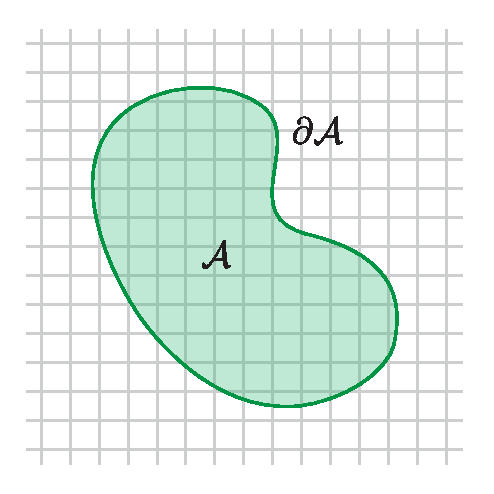
\includegraphics[width=\textwidth]{figs/december/entanglement-lattice.pdf}
		\caption{}
		\label{fig:entanglement-lattice}
	\end{subfigure}
	\begin{subfigure}[b]{0.45\textwidth}
		\centering
		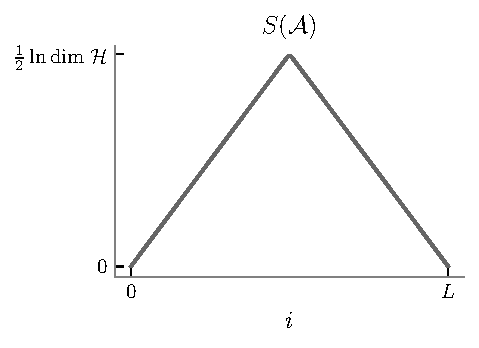
\includegraphics[width=\textwidth]{figs/december/page-curve.pdf}
		\caption{}
		\label{fig:entanglement-page-curve}
	\end{subfigure}
\end{figure}


\subsection{Entanglement in Lattice Systems} 
It is tradition to begin discussion of entanglement in quantum field theories 
by considering how one might define entanglement on a lattice.
From a conceptual point of view, lattice systems provide a natural way to define
and visualize entanglement entropy in quantum field theories. From a
calculational point of view, the presence of a lattice regularization makes
entanglement measures better behaved---in this setting they are finite, whereas,
as is typical for continuum QFTs, in the continuous case we find UV divergences 
which necessitate the introduction of some UV regularization, effectively limiting
the fastest modes of which we are allowed to measure entanglement. (Actually, 
the origin of UV divergences in entanglement entropies is a subtle and interesting 
point, especially in the case of CFTs, which are normally free of such pathologies.
We will discuss this in detail later.) 

Entanglement entropy is typically understood as the entropy of the density 
matrix that results from a partial trace over a subsystem. The standard treatment, 
readily found in any quantum information theory text, is as follows: Assuming 
there is a physically sensible Hilbert space factorization at hand, 
partition this factorization into a subsystem  $ \mathcal{A} $ and its complement $
\mathcal{A}^\complement $. Taking the total density matrix $ \rho $ and tracing
over the complement degrees of freedom yields a new reduced density matrix $
\Tr_{\mathcal{A}^\complement} \rho = \rho_\mathcal{A}$ whose spectrum is referred 
to as the \textbf{entanglement spectrum} (\cref{fig:entanglement-lattice}). This spectrum represents, of course,  
a mixed state whose entropy we can calculate; this is the \textbf{entanglement entropy}.

Lattice systems are a natural setting for this construction.
In particular, quantum lattice systems are defined by factorizable many-body 
Hilbert space
\begin{equation*}
	\mathcal{H} = \bigotimes_{i} \mathcal{H}_i
\end{equation*}
whose product structure makes defining a partial trace uncomplicated: we simply 
consider a subsystem $ \mathcal{A} $ consisting of a particular set of lattice sites, 
and trace over the degrees of freedom on the remaining lattice sites
(\cref{fig:entanglement-lattice}). Equipped with a spatial intepretation for the 
Hilbert space factorization, we can also outline the boundary of our subsystem,
$ \partial\mathcal{A} $, and understand it as the interface for quantum
information exchange between $ \mathcal{A} $ and $ \mathcal{A}^\complement $. 
For this reason it is referred to as the \textbf{entanglement surface}.

\begin{alertbox}[Aside: gauge theories]
	It is worth noting that for lattice gauge theories the above definition is not
	straightforward, and is the subject of ongoing research. The gauge field is
	formulated in terms of link variables that are situated \textit{between}
	lattice sites; thus, a partition of the lattice does not pick out a unique,
	gauge invariant partition of link variables, and one must make some choice
	as to the the subsystem the variable belongs in.
\end{alertbox}

\parhead{Scaling laws}
It is natural to ask how the entanglement entropy scales 
with the size of $ \mathcal{A} $. In one dimension, things are simple---$ \mathcal{A} $
is some chain of contiguous lattice sites, and the only real freedom in our 
partition is the location of $ \partial \mathcal{A} $, which is now a point. 
If we let this location be the site index $ i $ and measure the dependence of the 
entanglement entropy on the $ i $ (i.e., vary the fractional size of $ \mathcal{A} $),
we find a so-called \textbf{Page curve} which saturates the maximum entanglement
entropy---half the dimensionality of the total Hilbert space of the system---at
precisely halfway in the chain (\cref{fig:entanglement-page-curve}).

In higher dimensions the situation can be more interesting. We consider 
the thermodynamic limit of a $ D $ (spatial) dimensional system, and a subsystem
with linear size greater sufficiently larger than the lattice spacing: $ L \gg
a$. Under these conditions, most states in the Hilbert space will turn out to
possess a volume-law scaling, wherein the entanglement entropy is nearly
saturated, and $ S(\mathcal{A}) $ scales as the number of sites in the
subsystem, $ N_{\mathcal{A}} $:
\begin{equation*}
	S(\mathcal{A}) \propto N_{\mathcal{A}} \sim \frac{L^D}{a^D} 
\end{equation*}

Most physically realistic states, however---say, the ground state of a 
Hamiltonian---are subject to constraints that tie the lattice geometry to the 
entanglement struture in the form of some locality constraint. This is to say 
that entanglement should primarily be found between neighboring sites, or at 
least sites that are spatially near one another. This is the primary intuition 
behind \textbf{matrix product state} (MPS) ansatze and \textbf{tensor network theory}
formulations, wherein one builds wavefunctions with geometrically sound entanglement 
structures by placing tensors at each lattice site and contracting tensor indices 
between neighboring sites, i.e., creating a bond. This class of wavefunctions
occupies a relatively small corner of the Hilbert space and thus have seen much
recent success as a circumvention around the curse of dimensionality;
additionally, enforcing a degree of entanglement locality has proven a
successful recipe for many-body variational ansatze. 

The relevance of these states to entanglement scaling lies in the fact that we
can think of calculating the entanglement entropy by counting the number of
bonds cut by the boundary $ \partial \mathcal{A} $. In this case it is clear
that the entanglement entropy scales as the area of $ \mathcal{A} $:
\begin{equation*}
	S(\mathcal{A}) \sim  \frac{L^{D-1}}{a^{D-1}}.
\end{equation*}
It is commonly the case that gapped systems possess this entanglement scaling 
whereas gapless Hamiltonians in two dimensions tend to volume-law entanglement. 
Generally, there is a rich literature on entanglement scaling, network theory, 
and the like, and these points of view have grown increasingly central to modern 
many-body physics---especially when considering computational methods.
We have also neglected to mention topological entanglement entropies, which have 
played an integral role in recent developments in condensed matter physics, 
but this is a topic for a different occasion.

\begin{figure}[t]
	\centering
	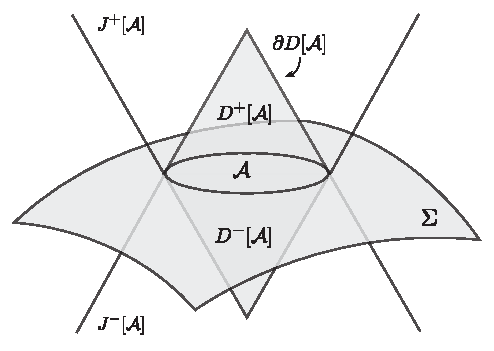
\includegraphics[]{figs/december/causal-structure.pdf}
	\caption{The causal struture of the subsystem $ \mathcal{A} $. 
	$ \Sigma $ is a Cauchy surface or slice, and $ \partial D[\mathcal{A}] $ is 
	the entangling surface. $ D^{\pm}[\mathcal{A}] $
	are the future and past domains of dependence---the regions of the manifold 
	where the content of the theory can be entirely determined by the configuration 
	on $ \mathcal{A} $. $ J^\pm[\mathcal{A}] $ are causal future and past, 
	the region of spacetime that is affected by the configuration on $ \mathcal{A} $.}
	\label{fig:entanglement-causal-structure}
\end{figure}

\parhead{Relativistic subsystems} In order to apply the preceding discussion 
to relativistic systems, it is necessary to develop a notion of subsystem that 
plays well with a spacetime picture. Actually, the best way to do this is by 
leveraging the causal structure of the underlying spacetime, whereby we find 
several additional features which refine our understanding of a subsystem 
in field theory. 

The natural extension of a lattice system like that of \cref{fig:entanglement-lattice} 
is a Cauchy slice $ \Sigma $, where a subsystem is some subset of the slice 
$ \mathcal{A} $. Causality leads to the constraint that no information from 
outside of $ \mathcal{A} $ can enter a lightlike codimension-$ 1 $ cones 
situated over $ A $ pointing in the positive and negative $ t $ direction; put 
differently, these are volumes where the content of the theory can be entirely 
determined by evolving the operator content of $ \mathcal{A} $ by the appropriate 
(presumably Heisenberg) equations of motion. These are of course the future 
and past domains of dependence $ D^{\pm}[\mathcal{A}] $ (or together $ D[\mathcal{A}]
= D^+ [\mathcal{A}] \cup D^- [\mathcal{A}]$) the content of which, 
again, is entirely determined by what is on $ \mathcal{A} $. We can also consider 
the region of spacetime that the content of $ \mathcal{A}$  may have an influence on, 
i.e., the union of the light cones of all points on $ \mathcal{A} $. These 
are the causal future and past $ J^{\pm}[\mathcal{A}] $. Then the natural 
extension of our entanglement surface is simply the boudnary of $ D[\mathcal{A}] $,
which we will denote $ \partial D[\mathcal{A}] = \partial \mathcal{A} $ for 
simplicity. 

This is the appropriate notion of a subsystem for a relativistic 
system (\cref{fig:entanglement-causal-structure}). Note that the choice of 
Cauchy surface is not unique: one can deform $ \Sigma $ while preserving the 
domain of dependence of $ \mathcal{A} $ and thus the entangling surface, so
that, to be pedantic, the proper way to think about a subsystem is in terms of
an equivalence class of Cauchy slices.

\subsection{Path integral techniques}
The entanglement entropy of continuum field theories is most conventiently 
calculated with a path integral formalism, usually because this admits a geometric 
picture which assigns clear interpretations to density matrix manipulations. 
To be specific, one identifies the matrix elements of a density matrix $\bra{\phi_1} \rho \ket{\phi_0}$
with boundary conditions on the path integral, then visualizes these conditions 
as cuts on the spacetime manifold. It is most convenient to imagine this in an
Euclidean setting by compactifing a complex time dimension $ t \rightarrow i\tau
\in [0, \beta] $, $ \beta\sim \beta + 2\pi $, so that the vacuum of the theory
may be studied by taking $ \beta \rightarrow \infty $ (corresponding to
flattening the temperature circle $ S^1 $ to $ \R $). Now the path integral 
calculates matrix elements of the canonical ensemble: $ \bra{\phi_1} e^{-\beta H}/ Z\ket{\phi_0} $.
This is kosher so long as we're interested in steady states of the theory---as 
the spectrum of the Hamiltonian is what enters the canonical density matrix---or when
considering an instantaneously static point in the spacetime manifold. 
{\color{myred} [go back to understand this]}

Let's make this formalism a little more explicit. Consider a $ 1+1 $ Euclidean 
field theory, and let $ \mathcal{A} $ be an interval of unspecified length living 
on some Cauchy slice which we can take to be $ \tau=0 $. We could like to 
calculate the matrix elements of the reduced density matrix $ \bra{\phi_1^\mathcal{A}}
\rho_{\mathcal{A}} \ket{\phi_0^\mathcal{A}} $, which is easy to convince oneself
amounts to setting boundary conditions on the interval (recall path integrals are 
essentially propagators) and fully integrating out the remainder of the field
configurations. In fact, generally the partial trace has the geometric 
interpretation of closing a cut made by matrix elements, as we will see later. 
Anyway, this is represented by 
\begin{align}
	\bra{\phi_1^\mathcal{A}} \Tr_{\mathcal{A}^\complement} e^{\beta H}/Z \ket{\phi_0^\mathcal{A}}
		&= \frac{1}{Z} \int_{\phi^\mathcal{A} = \phi^\mathcal{A}_0}^{\phi^\mathcal{A} = \phi^\mathcal{A}_0}
			\mathcal{D} \phi e^{S_{\text{E}}[\phi]}
		= \frac{1}{Z} \int
			\mathcal{D} \phi e^{S_{\text{E}}[\phi]} \; \delta (\phi_0,\phi_1)\nonumber\\ 
		&= \frac{1}{Z}\adjincludegraphics[valign=c]{figs/december/cylinder.pdf}\label{eq:entanglement-path-integral}
\end{align}
(actually in this figure $ \phi_0 $ and $ \phi_1 $ should be switched)
here the partition function $ Z $ has the interpretation of integrating over the
entire spacetime without any cuts, and the delta function $ \delta(\phi_0,\phi_1) $
provides a less schematic, more formal way of implementing the boundary
conditions. As a sanity check, we verify the Euclidean action $ S_{\text{E}} $
is really nothing more than the Hamiltonian: we can see this by writing the
action 
\begin{equation*}
	i \int d^d x \mathcal{L}[\phi]
		= i \int d^d \left(\partial_t^2 \phi - V[\phi]\right)
\end{equation*}
(here $ V[\phi] $ includes the spatial derivative terms) and seeing how 
it is transformed under $ t \rightarrow -i\tau $, 
\begin{equation*}
	\int d^{d-1}x \; d\tau \left(-\partial_\tau^2 \phi - V[\phi]\right)
		= - \int d^{d-1} x \; d\tau (\partial_t^2 + V[\phi])
		= -\int d^{d-1}x \; d\tau H[\phi].
\end{equation*}
 
\parhead{Replica trick} One computation that is made often in the entanglement 
entropy literature is that for the R\'enyi entropy via the replica trick. The 
idea is that while for the majority of field theories it is not quite clear 
how to compute the entanglement entropy, it is comparatively straightforward to 
compute the matrix elements of the $ n $-th power of the reduced density 
matrix, the log of the trace of which is the $ n $-th order R\'enyi entropy: 
\begin{equation*}
	S_{\text{A}}^{(n)}
		= \frac{1}{1-n} \ln \Tr \rho_\mathcal{A}^q
\end{equation*}
This is done by taking $ n $ copies of a path integral such as
\cref{eq:entanglement-path-integral} and implementing the matrix multiplication
by identifying the $ i $-th path integral's upper ($ \phi_1^i $) boundary condition with the 
$ i+1 $-th path integral's lower boundary condition ($ \phi_0^{i+1} $). E.g., 
\begin{equation*}
	\bra{\phi_1^2}\rho^2_\mathcal{A} \ket{\phi_0^1}= 
	\int \mathcal{D}\phi_1^1 
	\bra{\phi_1^2}\rho_\mathcal{A} \ketbra{\phi_1^1} \rho_\mathcal{A} \ket{\phi_0^1}
\end{equation*}
As we've stated above, by taking the trace over $ \rho_\mathcal{A}^2 $, we seal
the last cut in the $ n $ replicas and create a space without boundary.
A schematic of one such situation is displayed in \cref{fig:entanglement-replicas}.
Note that after taking the trace, the replicated system exhibits a so-called 
\textbf{replica symmetry}: we can shift the replicas cyclically and obtain the 
same result, so that the system possess a $ \Z_n $ ``symmetry.'' As it turns
out, the replica spacetime is now no longer formally a manifold:
we will later see how this constrution is equivalent to defining the theory on 
an orbifold, which surprisingly leads to significant calculational advantage.

\begin{figure}[t]
	\centering
	\begin{subfigure}[b]{0.4\textwidth}
		\centering
		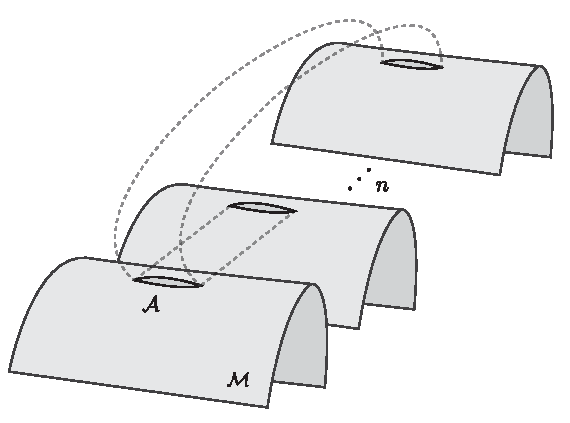
\includegraphics[width=\textwidth]{figs/december/replicas-cft.pdf}
		\caption{The $ n $-fold replica orbifold glued cyclically along the slits $ \mathcal{A} $.}
		\label{fig:entanglement-replicas}
	\end{subfigure}
	\hfill
	\begin{subfigure}[b]{0.49\textwidth}
		\centering
		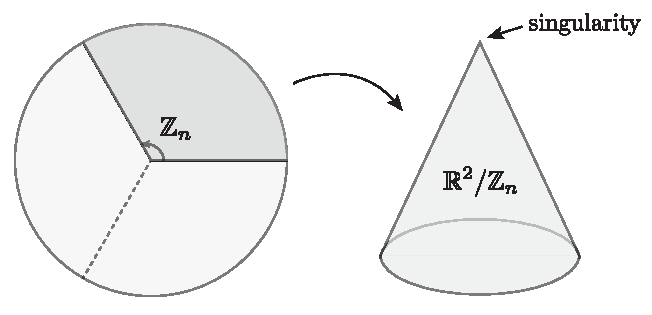
\includegraphics[width=\textwidth]{figs/december/cone.pdf}
		\caption{The cyclic orbifold $ \mathbb{R}^2/\mathbb{Z}_n $ is geometrically 
		a cone.}
		\label{fig:entanglement-cone}
	\end{subfigure}
\end{figure}

\subsection{Thermofield Double, Modular Hamiltonian}
There are two additional pieces of technology commonly employed in 
entanglement entropy calculations that are worth mentioning. The first 
is the \textbf{thermofield double}---which is a form of purification in the 
quantum information sense---a pure state constructed out of a thermal density 
matrix. The idea is to essentially write down a Schmidt decomposition out of 
two copies of a Hilbert space (hence ``double'') such that the partial trace 
over one of the copies yields the original canonical density matrix. 
Specifically the thermofield double is constructed by 
\begin{equation*}
	\rho_{\text{A}} = \frac{1}{Z} \sum_i e^{-\beta E_i} \ketbra{i}
	\quad\Longrightarrow \quad 
	\ket{\text{TFD}} = \frac{1}{\sqrt{Z}}\sum_ie^{-\frac{\beta}{2}E_i} \ket{i}
		\otimes \ket{i}
\end{equation*}
which lives in a double Hilbert space $ \mathcal{H}_{\mathcal{A}_1}\otimes 
\mathcal{H}_{\mathcal{A}_2}$ That this field is indeed a purification of $
\rho_{\mathcal{A}} $ can be seen by constructing the density matrix
\begin{equation*}
	\rho_{\text{TFD}} = \ketbra{\text{TFD}}
		= \frac{1}{Z} \sum_{ij} e^{-\frac{\beta}{2}(E_i + E_j)}
			\ket{i}\otimes \ket{i}\bra{j}\otimes \bra{j}
\end{equation*}
whose partial trace over $ \mathcal{H}_{\mathcal{A}_2} $ is 
\begin{equation*}
	\Tr_{\mathcal{A}_2}\rho_{\text{TFD}} \frac{1}{Z} =
		\sum_k e^{-\frac{\beta}{2}(E_i + E_j)} \braket{k}{i}\braket{j}{k}
			\ketbra{i}{j} 
		= \frac{1}{Z} \sum_k e^{-\beta E_k} \ketbra{k}.
\end{equation*}
The thermofield double is a useful construct because it functions as a bridge 
between thermal entropy calculations and entanglement entropy calculations: 
the thermal entropy of $ \rho_\mathcal{A} $ is exactly the entanglement entropy 
of $ \ket{\text{TFD}} $ over the copy Hilbert space.

The second tool is the \textbf{modular Hamiltonian}, which is the name given 
to the operator $ H_{\mathcal{A}} $ that satisfies 
\begin{equation*}
	\rho_\mathcal{A}
		= \frac{1}{Z}e^{-H_\mathcal{A}}
\end{equation*}
i.e., it is the Hamiltonian whose spectrum gives $ \rho_{\mathcal{A}} $ as a canonical density 
matrix (it is convention to absorb the inverse temperature into the definition 
of the Hamiltonian). Note that the von Neumann entropy can be retrieved as 
essentially the free energy corresponding to the modular Hamiltonian:
\begin{equation*}
	S_{\mathcal{A}}
	-\Tr \rho_\mathcal{A} \ln \rho_\mathcal{A} 
		= \Tr \rho_\mathcal{A} H_\mathcal{A}
			+ \Tr \rho\mathcal{A} \ln Z
		= \langle H_\mathcal{A} \rangle + \ln Z
\end{equation*}
This makes the modular Hamiltonian construction a sort of inverse problem of 
the thermofield double. This Hamiltonian is the subject of the famous
\textbf{Bisognano-Wichmann theorem}, an algebraic QFT result which states that
the modular Hamiltonian of certain field theories is nothing more than the
integral of the generator of Lorentz boosts. Besides this landmark result, the
modular Hamiltonian is frequently used to make nontrivial connections to bulk
physics in holographic scenarios; the precise nature of these considerations
lies outside the scope of the present discussion, but is nonetheless something I
am interested in understanding further.

In condensed matter literature, the modular Hamiltonian is better known as the 
\textit{entanglement Hamiltonian}. In this context, it has been applied to the 
problem of \textit{Hamiltonian reconstruction}: the question of whether it 
is possible to entirely determine a Hamiltonian from one of its ground states. 
See for instance, \href{https://journals.aps.org/prb/abstract/10.1103/PhysRevB.105.035106}{Biao Lian's paper} 
and references therein. A related approach which I studied extensively is the 
\textbf{correlation matrix} proposed by Qi and Ranard; it is an interesting 
line of inquiry---which I am currently exploring---to ask what the relationship 
between the correlation matrix and the modular Hamiltonian is, and whether 
these considerations can yield new insights into the gravity duals of holographic 
descriptions. 

\subsection{Example: the Rindler Wedge}
We now make a heuristic argument for the form of the modular Hamiltonian (and thus 
indirectly the entanglement entropy) of the simplest possible field theoretic 
example: the vacuum of a $ 1+1 $d field theory with $ \mathcal{A} $ the positive half line, 
$ x>0 $. In this case the domain of the dependence is the so-called
\textbf{Rindler wedge}: the region in the $ x>0 $ half of the $ x$-$t $ plane 
bounded from above by $ x=t $ and below by $ x=-t $. We will do this using the 
pictorial path integral formalism developed above; namely, we have an Euclidean 
thermal density matrix $ \rho = e^{-\beta H}/Z $ whose $ \beta \rightarrow \infty $
limit takes us to the vacuum $ \rho = \ketbra{0}{0} $ whose path integral is 
represented by
\begin{equation*}
	\bra{\phi_1}\rho\ket{\phi_0} = 
	\frac{1}{Z}\int_{\phi_0}^{\phi_1} \mathcal{D}\phi \; e^{S_{\text{E}}[\phi]}
	= \frac{1}{Z}
	\adjincludegraphics[valign=c, width=4cm]{figs/december/split-plane.pdf}
\end{equation*}
(here the $ \beta \rightarrow \infty $ limit has made the cylinder infinite in $
\tau $ extent). By performing a partial trace, we integrate over the field
configurations in the complement $ \mathcal{A}^\complement = \left\{x \mid
x<0\right\} $, so that the path integral is
\begin{align*}
\bra{\phi_1^\mathcal{A}}\rho_\mathcal{A}\ket{\phi_0^\mathcal{A}}
	= 
\bra{\phi_1^\mathcal{A}}\Tr_{\mathcal{A}^\complement}\rho\ket{\phi_0^\mathcal{A}}
= 
\adjincludegraphics[valign=c, width=4cm]{figs/december/half-split-plane.pdf}
\end{align*}

Now, by inspecting this cut spacetime we can guess that the appropriate way to 
treat it is by switching to radial coordinates 
\begin{equation*}
	x = r \cos\theta, \quad \tau = r \sin\theta
\end{equation*}
where $ \theta $ is, as pictured, taking us from one boundary condition to another. 
In fact, we can go farther and immediately Wick rotate this coordinate 
system back to Minkowski signature. There is an ambiguity in what we choose 
as a time coordinate {\color{myred}[I did not know this; investigate futher]}, 
and we can Wick rotate $ \theta $ itself to $ \theta= i\chi $. Under this 
transformation we have 
\begin{equation*}
	x = r\cosh \chi,\qquad t = -i\tau = r\sinh \chi
\end{equation*}
where we've used $ \cos ix = \cosh x $, and $ -i\sin i x = \sinh x $. Now, 
the linear coordinates transform under boosts (written in the form of a rapidity $ \eta $) as
\begin{equation*}
	\begin{cases}
	t' = \cosh \eta \; t + \sinh \eta \; x  \\ 
	x' = \sinh \eta \; t + \cosh \eta \; x
	\end{cases}
\end{equation*}
so that the radial coordinate is unchanged
\begin{align*}
	r' = x'^2 - t'^2 
		&= (\sinh \eta \; t + \cosh \eta \; x)^2 
			- (\cosh \eta \; t + \sinh \eta \; x)^2\\
		&= \sinh^2 \eta \; t^2 + 2\sinh\eta \cosh \eta \; xt 
			+ \cosh^2 \eta \; x^2\\
		 &\qquad - \sinh^2 \eta \; t^2 - 2\sinh\eta \cosh \eta \; xt 
			- \cosh^2 \eta \; x^2\\
		&= (\cosh^2 \eta - \sinh^2 \eta )x^2 +
			(\sinh^2 \eta - \cosh^2 \eta) t^2 
		= x^2 - t^2
\end{align*}
and the Minkowski radial coordinates are shifted linearly:
\begin{align*}
	\tanh \chi' 
		&= \frac{t'}{x'} = \frac{\cosh\eta \; t + \sinh \eta \; x}{\sinh \eta \; t + \cosh \eta \; x}
		= \frac{\cosh \eta \sinh \chi + \sinh \eta \cosh \eta}{\sinh \eta \sinh \chi 
			+ \cosh \eta \cosh \chi}\\ 
		&= \frac{\sinh(\chi + \eta)}{\cosh(\chi + \eta)}
		\Longrightarrow 
		\tanh \chi ' = \tanh(\chi - \eta).
\end{align*}
We can therefore identify $ \chi $ as none other than the rapidity of this 
coordinate system. If this seems unsavoury, recall that the boost is nothing 
more than a hyperbolic rotation, such that just as $ \theta $ might parametrize 
a coordinate system that can be rotated, $ \chi $ can parameterize a Lorenz frame. 
Just as the generator of time translations appears in the exponential of the 
canonical density matrix, the generator of boosts here then plays the role of a 
modular Hamiltonian with temperature $ \beta = 2\pi $ (for we have rotated across 
the whole plane)
\begin{equation*}
	\rho_\mathcal{A} = \frac{1}{Z} e^{-2\pi K}
\end{equation*}
This is a manifestation of the aformentioned Bisognano-Wichmann theorem. In fact, 
this result gives us even more: The $ \beta=2\pi $ looks awfully familiar; indeed, let us 
consider the worldline of an observer confined to the Rindler wedge. One such 
worldline is a line of constant $ r $: 
\begin{equation*}
	r = \sqrt{x^2 - t^2} \Longrightarrow x = \sqrt{r^2 + t^2}
\end{equation*}
which one can verify is that of an observer with proper acceleration 
$ a=1/r $. Thus we have just recovered the Unruh effect---this observer sees 
a thermal density matrix with temperature $ a/2\pi $ (the $ a $ comes from a 
redshift correction), the interpretation being that to the observer, the 
modes of the vacuum entangled with the complement of the Rindler wedge have
decohered and given rise to a canonical ensemble. Indeed, it is not difficult 
to see how any observer strictly confined to the Rindler wedge must necessarily 
be accelerating.

It is worth briefly mentioning how 

\subsection{Cardy-Calabrese Formula}
To illustrate how the replica trick is employed to calculate entanglement 
entropies, we derive the classic Cardy-Calabrese entropy for an interval 
on a $(1+1)$d CFT. We seek to compute the $ n $-th order R\'enyi entropy by 
evaluating the partition function 
\begin{equation}\label{eq:entanglement-renyi-partition}
	\Tr \rho^n_\mathcal{A} = \frac{Z_n[\mathcal{A}]}{Z[\mathcal{M}]^n}.
\end{equation}
Here $ Z_n [\mathcal{A}] $ denotes the partition function over $ n $ copies 
of the spacetime manifold $ \mathcal{M} $ glued along a cut on the subsystem $
\mathcal{A} $. Here we take $ \mathcal{A} = -\ell/2 < x < \ell / 2 $, a length-$
\ell $ interval at $ t=0 $, and $ \mathcal{M} $ is the complex plane. The
denominator $ Z[\mathcal{M}]^n $ is the $ n $-th power of partition function
over $ \mathcal{M} $ coming from the normalization over each subsystem partition 
function---note that this implicitly includes the order-$ n $ branch along which 
the replicas are glued. The advantage of this construction is it admits a
description in terms of orbifold theory, allowing us to import powerful tools
from that formalism. In particular, we can view the numerator as a \textit{cyclic
orbifold CFT} $ \mathcal{M}/Z_n $ with fixed points along the interval $
\mathcal{A} $. In fact, in this language, we can more clearly see that the replica 
gluing procedure introduces conical singularities at the endpoints of the interval 
$ \mathcal{A} $---we recognize that the quotient $
\mathcal{M}/\mathbb{Z}_n $ is geometrically a cone with excess angle $ 2\pi
(1-1/p) $ \mycite{Caramello}. These will turn out to induce a Weyl anomaly  
which lies at root of the UV divergence in the entanglement entropy.

The more practical advantage of this orbifold formulation is that it permits a 
direct calculation of the partition function. We do this by way of formal 
\textit{twist operators} $ \mathcal{T}_n(x,t) $, $ \mathcal{T}_{-n}(x,t) $ whose
insertions\footnote{When people refer to an ``insertion'' of an operator 
$ \mathcal{O} $ at a spacetime point $ (x,t) $ they mean a calculation of the
expectation value $ \mathcal{O}(x,t) $ by way of ``inserting'' the operator 
into the partition function.} create the endpoints of an order $ n $
branch point on the manifold and thus produce $ \mathcal{M}/\mathbb{Z}_n $. 
The replica partition function is then exactly the insertion 
\begin{equation*}
	Z_n[\mathcal{A}]
		= \langle \mathcal{T}(-\tfrac{\ell}{2}, 0) \mathcal{T}(\tfrac{\ell}{2}, 0) \rangle
\end{equation*}
Of course, the advantage of working with a CFT is we have precise knowledge of 
two point correlators. We find that assuming these are primary operators with 
conformal dimension $ h_{\mathcal{T}}=\bar{h}_{\mathcal{T}} $
\begin{equation*}
	\langle \mathcal{T}(-\tfrac{\ell}{2}, 0) \mathcal{T}(\tfrac{\ell}{2}, 0) \rangle
		= \frac{1}{\ell^{4h_{\mathcal{T}}}}.
\end{equation*}
Now it remains to determine the conformal dimension $ h_{\mathcal{T}} $. Here we reproduce the 
argument given in \mycite{Estiene}: we impose periodic boundary conditions with 
length $ L $ so that the theory is
\begin{equation*}
	H = \frac{2\pi}{L} \left(L_0 + \bar{L}_0 - \frac{nc}{12}\right)
\end{equation*} 
(see Di Francesco \S11.3.2). Here $ L_0 $, $ \bar{L}_0 $ are elements of the 
two copies of the Virasoro algebra of this theory; in the radial quantization, 
their sum is the generator of time translations and thus is identified as 
the Hamiltonian. The presence of $ n $ replicas produces a central charge 
$ nc $, where $ c $ is the central charge of the original theory. By construction, 
the twist operator $ \mathcal{T} $ is associated with (i.e.,
creates/annihilates) the vacuum of the twisted theory, which with $ L_0
\ket{h_{\mathcal{T}}} = h\ket{h_{\mathcal{T}}} $
has energy 
\begin{equation*}
	E = \frac{2\pi}{L} \left(2 h_{\mathcal{T}} - \frac{nc}{12}\right).
\end{equation*}
At the same time, this theory can be unwrapped to a single theory with period $
nL $ with Hamiltonian 
\begin{equation*}
	H = \frac{2\pi}{nL} \left(	L_0 + \bar{L}_0 - \frac{c}{12}\right)
\end{equation*}
whose vacuum posseses vanishing conformal weight, and thus has energy 
\begin{equation*}
	E = -\frac{2\pi}{nL}\frac{c}{12}
\end{equation*}
Equating the two energies then obtains 
\begin{align*}
	\frac{4\pi}{L} \left(2h_{\mathcal{T}} - \frac{nc}{12}\right)
		&= \frac{4\pi}{nL} \frac{c}{24} \\
	 2h_{\mathcal{T}} - \frac{nc}{12} &= \frac{c}{24 n}
	\quad\Longrightarrow \quad
	h_{\mathcal{T}}
		= \frac{c}{24}(n - \tfrac{1}{n}).
\end{align*}
Thus the partition function is 
\begin{equation*}
	Z_n[\mathcal{A}]
		= \langle \mathcal{T}(-\tfrac{\ell}{2}, 0) \mathcal{T}(\tfrac{\ell}{2}, 0) \rangle
		= \frac{1}{\ell^{\frac{c}{6}(n-\frac{1}{n})}}.
\end{equation*}
We have evaluated the numerator of \cref{eq:entanglement-renyi-partition} 
and should in principle be set to state the R\'enyi entropy of the interval of a 
CFT. However, an additional subtlety arises from the denominator $ Z[\mathcal{M}]^n $: 
as stated above, the branch cut created in the replica trick produces conical 
singularities in the underlying manifold $ \mathcal{M} $ located at the endpoints 
of the interval. These are geometric singularities (i.e., singularities in the 
metric) which induce a diverging curvature and thus must be regularized in our 
integration of the partition function---the obvious choice is to omit a
disc of radius $ \epsilon $ around the singularity. Any such regularization will, 
however, introduce a length scale to our theory and will induce a conformal (or
Weyl) anomaly in the CFT. Put differently, while the lack of a length scale 
in CFTs on better-behaved (flat, nonsingular) spacetimes generally leads to a 
finite partition function, any regularization introduced to handle singularities
will break scale invariance and thereby lead to a conformal anomaly which lies 
at the root of the UV-divergences in entanglement entropy calculations of this 
sort.
Thus, we write 
\begin{equation*}
	\Tr \rho^n_{\mathcal{A}} 
		= \frac{Z_n[\mathcal{A}]}{Z[\mathcal{M}]^n}.
		=  \left(\frac{\ell}{\epsilon}\right)^{\frac{c}{6}(n- \frac{1}{n})}
\end{equation*}
which leads naturally to the R\'enyi entropy
\begin{align*}
	S^{(n)}_A &= \frac{1}{1-n}\ln \Tr \rho_\mathcal{A}^n 
		= - \frac{1}{1-n} \cdot \frac{c}{6}\left(n - \frac{1}{n}\right)\ln \frac{\ell}{\epsilon} + \cdots \\
		&= \frac{n+1}{n^2 - 1} \cdot \frac{1}{n}(n^2 - 1) \cdot \frac{c}{6}\ln \frac{\ell}{\epsilon} + \cdots\\
		&= \frac{c}{6}\left(1 + \frac{1}{n}\right) \ln \frac{\ell}{\epsilon} + \cdots
\end{align*}
(the ellipses hide terms coming from the details of the regularization). This is
the desired Cardy-Calabrese formula. The von Neumann entropy is simply the
analytic continuation to $ n=1 $:
\begin{equation*}
	S_\mathcal{A} = \frac{c}{3} \ln \frac{\ell}{\epsilon}.
\end{equation*}
While the continuation is trivial in this case, this is a peculiarity of the 
constrution under study that is typically absent in calculations for more 
complicated subsytem topologies. We can, however, modify the topology of the 
underlying spacetime without much difficulty; it turns out that, had we 
considered $ \mathcal{M} $ compact in one dimension, say $ \mathcal{M} = 
\mathcal{R} \times S^1$ with circumference $ \ell_{S^1} $, we would have found 
\begin{equation*}
	S_\mathcal{A}
		= \frac{c}{3} \ln \left(\frac{\ell_{S^1}}{\pi \epsilon} 
			\sin \frac{\ell}{\ell_{S^1}}\right)
\end{equation*}
and the change $ \ell_{S^1} = i\beta $ then allows us to find the entanglement 
entropy of a thermal system with inverse temperature $ \beta $.

\subsection*{References}
\begin{itemize}[nosep]
\item Rangamani, Takayanagi, \textit{Holographic Entanglement Entropy} (2017).
\item Headrick, \textit{Lectures on Entanglement Entropy in Field Theory and 
	Holography} (2019),
\href{https://arxiv.org/abs/1907.08126}{[arXiv:1907.08126]}.  
\item Estiene, Ikhlef, Rotaru, \textit{The operator algebra of cyclic orbifolds} (2023), 
	\href{https://arxiv.org/abs/2212.07678}{[arxiv:2212.07678]}.
\item Calabrese, Cardy, \textit{Entanglement Entropy and Quantum Field Theory} (2004),
	\href{https://arxiv.org/abs/hep-th/0405152}{[arXiv:hep-th/0405152]}.
\item Calabrese, Cardy, \textit{Entanglement Entropy and Conformal Field Theory} (2009),\\ 
	\href{https://arxiv.org/abs/0905.4013}{[arXiv:0905:4013]}.
\item Caramello, \textit{Introduction to Orbifolds} (2019),
	\href{https://arxiv.org/abs/1909.08699}{[arXiv:1909.08699]}.
\end{itemize}

\section{AdS/CFT, Roughly} 
In what follows we introduce famous AdS/CFT correspondence, first giving some 
motivation for the duality, then by describing the most general situation 
in which such correspondences exist.

\subsection{Anti-de Sitter Space}
\begin{table}
\centering
\begin{tabular}{c| c| c}
& Embedded in $ R^{d+1} $ & Embedded in $ \text{Mink}_{d+1} $ \\\hline 
Intrinsically Euclidean  & $ S^d $ & Hyperbolic\\
Intrinsically Minkowski  & $ \text{dS}_d $ & $ \text{AdS}_{d} $
\end{tabular}
\caption{}
\label{tab:ads-table}
\end{table}
We assume the reader has a degree of familiarity with conformal field theory 
and, and instead focus on providing background on the spacetime that admits the
correspondence: anti-de Sitter space. It is most convenient to imagine 
$ d $ dimensional anti-de Sitter ($ \text{AdS}_d $) as the metric for a surface
embedded in some $ d+1 $ dimensional ambient space, much like how $ S^d $ might 
be embedded in $ \R^{d+1} $ by subjecting the coordinates to the constraint 
$ \sum x_i^2 = R^2 $. In fact, the analogy can be taken further: We can 
embed not only the sphere but also a hyperbolic space of constant negative 
curvature, the latter being subject to the constraint 
\begin{equation*}
	\sum_{i=1}^{d-1} x_i^2  - x_d^2 = -R^2
\end{equation*}
and embedded not in $ \R^{d+1} $ but in $ \text{Mink}_{d+1} $.
Then we can take the sphere to de Sitter space and the hyperbolic space 
anti-de Sitter space by Wick rotating one of the coordinates of the embedded 
surfaces. See \cref{tab:ads-table}. Then $ \text{AdS}_{d} $ lives in a space 
with metric 
\begin{equation*}
	ds^2 = -dx^2 + dx_1^2 + \cdots - dx_{d+1}^2
\end{equation*}
subject to the constraint 
\begin{equation*}
	-x_0^2 + x_1^2 + \cdots - x_{d+1}^2 = -R^2
\end{equation*}
This is an extrinsic characterization of the space; any intrinsic characterization 
will depend on some choice of coordinates, the most common choice (and the choice 
that typically serves as the backdrop of AdS/CFT) are the \textbf{Poincar\'e coordinates}
\begin{equation*}
	ds^2 = -\frac{R^2}{z^2}\left(-dt^2 + \sum_{i=1}^{d-2}dx_i^2 + dz^2 \right).
\end{equation*}
Here $ z\in (0,\infty) $, and, if we consider a constant $ t $ slice such that 
$ dt=0 $, we find that this is the metric of the Poincare half-plane. From this 
it is clear the sense in which the space possesses constant negative curvature; 
it is also clear that, by converting the half-plane to the Poincar\'e disk, 
one can obtain the famous model of AdS consisting of a temporal stack of 
hyperbolic disks. The coordinate system we have chosen does not, however, cover 
the entirety of $ \text{AdS}_{d} $---the $ z $ coordinate finds the boundary of 
the AdS cylinder (the conformal boundary) at $ z=0 $, but only goes as far as
lightlike hyperplanes slicing across the cylinder at $ z=\infty $. The region
the coordinates cover is referred to as the \textbf{Poincar\'e patch}. 

The holographic boundary theory of the bulk Poincar\'e patch theory will turn
out to be Minkowski space $ \text{Mink}_{d-1} $. There is an alternate
coordinate system which does cover the entirety of the $ \text{AdS}_{d} $;
however, interestingly enough, the holographic theory 
induced by this coordinatization is not set on Minkowski space but instead on an
Einstein static universe $ \R \times S^{d-2} $. The details can be found 
in Rangamani and Takayanagi's book.

\subsection{Some motivation for AdS/CFT}
The anti-de Sitter/conformal field theory correspondence asserts that a theory
of quantum gravity in asymptotically AdS spacetime (referred to as the bulk) can
be entirely encoded in a a conformal field theory living on the AdS boundary
(referred to as the boundary). There are additional constraints on the both 
theories that must be fulfilled for the duality to hold, and various theories in
either the bulk or the boundary fit are capable of fitting into the
correpondence. Here we motivate AdS/CFT with the example that Juan Maldacena
originally gave---$ 3+1 $d $ \mathcal{N}=4 $ supersymmetric Yang-Mills (SYM) on the boundary and 
type IIB supergravity in the bulk. Crucial to the correspondence is the fact 
that both theories are limits of type IIB string theory in a sense that will be
made exact shortly, and the observation made by \href{https://arxiv.org/abs/hep-th/9510017}{Polchinski}
that in type II string theory there is an equivalence between $ D3 $-branes and
extremal black $ p $-branes.

The (charged) $ D3 $-brane in $ \mathcal{R}^{1,9}=\text{Mink}_{10} $ produces the metric
\begin{equation*}
	ds^2 = H^{-1/2} (r) \;  d\textbf{x}^2 + H^{1/2}(r)(dr^2 + r^2 d\Omega_5^2),\qquad 
	H(r) = 1 + \frac{R^4}{r^4},\quad R = 4\pi g_{\text{s}} N \alpha'^2
\end{equation*}
where $ \alpha' $ is the Regge slope, $ g_{\text{s}}$ is the string coupling, and $ N $
counts the number of $ D3 $-branes stacked here. First note that in the 
$ r \rightarrow 0 $ limit---i.e., close to the $ D3 $-brane, we have 
$ H(r) \sim R^4/r^4 $, and letting $ r/R = r/z $: 
\begin{equation*}
	ds^2 = \frac{R^2}{z^2}\left(-dt^2 + d\textbf{x}_3 + dz\right) + R^2 d\Omega_5^2
\end{equation*}
so this is asymptotically $ \text{AdS}_5\times S^5 $.

At low energies--equivalent by dimensional analysis to $ 4\pi g_{\text{s}} N \ll
1 $---the string endpoints on the $ D3 $-branes are known to be described by an
$ \text{SU}(N) $ $ \mathcal{N}=4 $ SYM with 't Hooft coupling $ \lambda = 4\pi
g_{\text{s}}N $. The condition $ \lambda \ll 1 $ is associated with a large 
$ N $ limit of SYM.
From the equivalent point of view of the $ p $-branes, the high curvature 
in the $ r \rightarrow 0 $ limit is associated low energy fluctuations about 
the $ \text{AdS}_5 \times S^5 $ background. It is this correspondence that 
motivates AdS/CFT.

\parhead{GPKW prescription} The correspondence can be made precise at the level 
of the Euclidean partition functions using the GPKW prescription, which states that 
when considering an operator $ \mathcal{O} $ sourced by a current $ J$ in the 
boundary theory: 
\begin{equation*}
	Z_{\text{CFT}}[J]
		= \int \mathcal{D}[\text{CFT fields}] \exp \left(
			S_{\text{CFT}} + \int \mathcal{O} (x) \mathcal{J}(x)
		\right)
\end{equation*}
we can equate this partition function with that for the string theory on the 
AdS background for a string field $ \phi $ with boundary value $ J $: 
\begin{equation*}
	Z_{\text{CFT}}[J] = Z_{\text{string}}[\phi(J)]
\end{equation*}
But since we consider the classical gravitational theory, we can go one 
step further and simply equate this to the saddle-point solution
\begin{equation*}
	Z_{\text{CFT}}[J] = e^{-S_{\text{classical}}[\phi(J)]}.
\end{equation*}

\subsection{Ryu-Takayanagi Formula}
In context of entanglement entropy, the cornerstone of holographic methods is 
the Ryu-Takayanagi formula, which is a remarkable generalization of the
Bekenstein-Hawking formula relating the area of the black hole horizon to the
thermal entropy at the horizon. 
It suffers from the limitation that the boundary geometry must be static, but 
generalizations (the Hubeny-Ryu-Takayanagi formula) exist, and nonetheless 
it is a powerful result.  The demonstration is quite involved and technical, 
so we opt to state the result and make some comments on how it is derived.

The Ryu-Takayanagi formula states that the entropy of a subsystem $ \mathcal{A} $
living on the boundary theory is given by the area of the minimal surface whose 
boundary is the entanglement surface $ \partial  A $: 
\begin{equation*}
	S(\mathcal{A}) = \frac{1}{4G_{\text{N}}} \text{area}\;(\min \mathcal{A})
\end{equation*}
Besides bearing $ \partial \mathcal{A} $ as a boundary, the surface is additionally 
required to obey a so-called homology constraint stating the it must be homologous 
to $ \mathcal{A} $; while it is tempting to think of this as meaning ``related by a
continuous deformation'' in the sense of a homotopy class, homologous spaces 
are not always homotopic despite homotopic implying homologous. 

The Ryu-Takayanagi formula is an example of a boundary calculation that is
significantly easier to do in the bulk theory. This is rooted in arguments that 
the analytical continuation necessary to take us to the von Neumann entropy 
from the R\'enyi entropy is easier to perform in the bulk theory. At any rate, 
the argument is ``simply'' to consider an orbifold calculation of the partition 
function for the R\'enyi entropy, and use the GPKW prescription to contruct a
brane homologous to $ \mathcal{A} $. The string partition function is then 
solved by a saddle-point approximation which can be shown to be equivalent to 
a minimal surface condition. Details and extensions are found in Rangamani and 
Takayanagi's book.

\section{Weyl/Conformal Anomalies}

\chapter{Miscellany}
$ \text{SO}(n+1)/\text{SO}(n) = S^n $ ($ n $-sphere), from Natase book on 
string theory. 

The difference between Weyl and conformal invariance is that conformal transformation 
is an actual change of coordinates (like you are mapping from one set of coordinates 
to another, literally look at the equation!) that happens to result in a scaling 
of the metric, whereas Weyl transformation is a literal explicit change in 
the metric. 

When people say pick a foliation of spacetime, they mean this is necessary 
in order to preserve causalityl.
\end{document}